\documentclass[a4paper,12pt,twoside,brazil]{icmc}
%{icmc}

\usepackage{amsmath}
\usepackage{color}
\usepackage{colortbl}
\usepackage[top=20mm,bottom=20mm,left=20mm,right=15mm]{geometry} %coloca o tamanho das margens
\usepackage{setspace} %espacamento entre linhas
\usepackage{natbib} %referencias com numera\c{c}\~{a}o
 
\usepackage[utf8]{inputenc}
\usepackage[brazil]{babel}
%\let\cite=\citep
\usepackage{url}
\usepackage{listings}
% \lstset{language=[AspectJ]Java, stringstyle=\ttfamily,basicstyle=\ttfamily, showstringspaces=false}
\usepackage{fancybox}
\usepackage{indentfirst} %indenta a primeira linha
\usepackage{times}       %utiliza a fonte Times New Roman
\usepackage{titlesec} %para os gr\'{a}ficos dos cap\'{\i}tulos
\usepackage{textfit}
\usepackage{fancyhdr} % Para colocar cabe\c{c}alho nas p\'{a}ginas
\usepackage{subfigure}
\usepackage{lettrine} % Para fazer letras capitulares
\usepackage{lscape}

\usepackage{lmodern} % fonte CMR que funciona

 \usepackage {pdfsync} 
 
%\usepackage[default]{droidserif}
\usepackage[T1]{fontenc}

\usepackage[pdftex]{hyperref}
\usepackage[pdftex]{graphicx} %pacote para incluir imagens

%\hypersetup{colorlinks=true,debug=false,
%             linkcolor=black,%%%cor do tableofcontents,\ref,\footnote,etc
%             citecolor=black, %%% cor do \cite
%             urlcolor=black, %%% cor do \url e \href
%             pdftitle={Geração de aplicações para linhas de produtos orientadas a aspectos com apoio da ferramenta Captor-AO},
%             pdfauthor={Carlos Alberto de Freitas Pereira Júnior},
%             pdfsubject={Programação Orientada a Aspectos e Geradores de Aplicações}}

\newcommand{\fig}[1]{\textit{fig.~\ref{#1}}}

%% Uso do comando: Na \fig{fig:xxxx} é apresentada...
%\newcommand{\aspas}[1]{``#1''} %% Uso do comando: O termo \aspas{feature} é utilizado...

\newcommand{\fonte}[1]{
	\centering
	\fontfamily{cmss}\selectfont
	\footnotesize{
			\textbf{Fonte: \textnormal{
				\fontfamily{cmss}\selectfont
				\footnotesize{#1}
			}
		}
	}
}

\newcommand{\foot}[1]
{
	\footnote{
		\fontfamily{cmss}\selectfont
		\footnotesize{#1}
	}
}

\fontfamily{cmss}\selectfont

\begin{document}

%\hyphenation{res-pei-to abs-tra-\c{c}\~{a}o su-ges-t\~{o}es
%cons-tru-\'{i}-do En-ge-nha-ri-a ca-mi-nhos pre-o-cu-pa-ram}

%\begingroup

\pagestyle{empty}

\
\vfill
\begin{center}
\begin{minipage}[c]{12cm}
\begin{center}
\hrulefill\\
\vspace{.5cm} {\Large\sf{Navegação de Veículos Autônomos em Ambiente Externo Não Estruturado baseada em Visão Computacional}}\\
\vspace{1.3cm}
\textbf{\large\textit{Rafael Luiz Klaser}}\\
\vspace{.5cm}
\hrulefill\\
\end{center}
\end{minipage}
\end{center}
\vfill

\cleardoublepage

%\include{rosto}

%\include{agradecimentos}
%\newpage\ \thispagestyle{empty}

\frontmatter


\begin{resumo}

O objetivo deste trabalho é pesquisar, propor e desenvolver um sistema que
capacite um veículo terrestre a se locomover de modo autônomo em ambientes
externos não estruturados ou pouco estruturados, ou seja, em um campo com
vegetação/plantação e/ou em uma floresta pouco densa (\textit{outdoor} e
\textit{off-road}). O veículo deverá ser capaz de se dirigir até uma localização
pré-determinada (coordenada GPS) escolhendo por meios próprios o caminho a
seguir, ao mesmo tempo em que desvia de obstáculos, percebendo-os de forma
autônoma. O sistema de navegação autônoma irá se basear na aquisição e
processamento de imagens, obtidas a partir de um par de câmeras (câmera
estéreo), constituindo assim um sistema de visão binocular do qual é possível se
obter uma percepção tridimensional do ambiente. Portanto, pretende-se extrair
parâmetros de navegabilidade do ambiente percebido pela câmera estéreo, como
caminhos livres, obstruções e obstáculos, que combinados com as informações de
posição e orientação do veículo e do ponto de destino (baseando-se em
coordenadas de GPS) serão integrados em um sistema robusto de navegação.

% Este trabalho irá utilizar a plataforma CaRINA I do LRM-ICMC/USP e INCT-SEC
% dotado de uma câmera estéreo, GPS e bússola, e atuadores usados para o
% controle de tração e direcionamento do veículo.
Inicialmente serão estudados e trabalhados algoritmos para a criação do mapa de
disparidade a partir do par de imagens obtidas pela câmera estéreo.
% Para a criação deste mapa o algoritmo deverá ter um compromisso de desempenho
% entre a qualidade (disparidade/profundidade) e a performance em termos de
% tempo de processamento, uma vez que a aplicação final deverá executar em tempo
% real (\textit{soft real-time}).
A partir do mapa de disparidade, será elaborado um mapa local de navegabilidade
que irá processar e classificar o espaço tridimensional percebido, separando e
representando as regiões navegáveis (seguras) e as regiões não navegáveis
(obstáculos e regiões à evitar) do espaço em frente ao veículo. Este mapa local
será utilizado em conjunto com as informações de posição atual e de destino (GPS
e bússola) a fim de realizar o controle da navegação do veículo. Estão sendo
consideradas duas abordagens principais para o controle local da navegação: a
primeira baseada no uso de Redes Neurais Artificiais, conforme proposto em
trabalhos anteriores desenvolvidos por membros do grupo do LRM e a segunda
baseada em uma adaptação do algoritmo VFH. Nestas abordagens serão consideradas
como parâmetro de entrada as informações tridimensionais do mapa de
navegabilidade.
% Além disto, também serão necessários estudos que visam identificar, a partir
% das imagens da câmera estéreo, o plano de referência de base (chão), seus
% desníveis e obstáculos, classificando-os como elementos transponíveis ou não.
As principais contribuições esperadas deste trabalho são a adaptação e
aperfeiçoamento dos algoritmos para a geração de mapas de disparidade, a
proposta e o desenvolvimento de algoritmos para a obtenção de mapas locais de
navegabilidade com informações espaciais (3D), e por fim o aperfeiçoamento de
técnicas previamente desenvolvidas para detectar e desviar de obstáculos em
mapas 2D, a fim de permitir uma navegação baseada no mapa de navegabilidade 3D.

%Este trabalho resultará em um sistema com
%possibilidade de aplicação em importantes tarefas de navegação, como por
%exemplo, em sistemas voltados para aplicações agrícolas e em sistema de combate
%a incêndio em florestas.

\end{resumo}

% 2012-10-10 lido ok

%\newpage\ \thispagestyle{empty}
%\include{abstract}
%\newpage\ \thispagestyle{empty}


%\tableofcontents 
%\newpage\ \thispagestyle{empty}
%\listoffigures 
%\newpage\ \thispagestyle{empty}
%\listoftables
%\newpage\ \thispagestyle{empty}

%\endgroup


\mainmatter

% capítulos
%\begin{resumo}

O objetivo deste trabalho é pesquisar, propor e desenvolver um sistema que
capacite um veículo terrestre a se locomover de modo autônomo em ambientes
externos não estruturados ou pouco estruturados, ou seja, em um campo com
vegetação/plantação e/ou em uma floresta pouco densa (\textit{outdoor} e
\textit{off-road}). O veículo deverá ser capaz de se dirigir até uma localização
pré-determinada (coordenada GPS) escolhendo por meios próprios o caminho a
seguir, ao mesmo tempo em que desvia de obstáculos, percebendo-os de forma
autônoma. O sistema de navegação autônoma irá se basear na aquisição e
processamento de imagens, obtidas a partir de um par de câmeras (câmera
estéreo), constituindo assim um sistema de visão binocular do qual é possível se
obter uma percepção tridimensional do ambiente. Portanto, pretende-se extrair
parâmetros de navegabilidade do ambiente percebido pela câmera estéreo, como
caminhos livres, obstruções e obstáculos, que combinados com as informações de
posição e orientação do veículo e do ponto de destino (baseando-se em
coordenadas de GPS) serão integrados em um sistema robusto de navegação.

% Este trabalho irá utilizar a plataforma CaRINA I do LRM-ICMC/USP e INCT-SEC
% dotado de uma câmera estéreo, GPS e bússola, e atuadores usados para o
% controle de tração e direcionamento do veículo.
Inicialmente serão estudados e trabalhados algoritmos para a criação do mapa de
disparidade a partir do par de imagens obtidas pela câmera estéreo.
% Para a criação deste mapa o algoritmo deverá ter um compromisso de desempenho
% entre a qualidade (disparidade/profundidade) e a performance em termos de
% tempo de processamento, uma vez que a aplicação final deverá executar em tempo
% real (\textit{soft real-time}).
A partir do mapa de disparidade, será elaborado um mapa local de navegabilidade
que irá processar e classificar o espaço tridimensional percebido, separando e
representando as regiões navegáveis (seguras) e as regiões não navegáveis
(obstáculos e regiões à evitar) do espaço em frente ao veículo. Este mapa local
será utilizado em conjunto com as informações de posição atual e de destino (GPS
e bússola) a fim de realizar o controle da navegação do veículo. Estão sendo
consideradas duas abordagens principais para o controle local da navegação: a
primeira baseada no uso de Redes Neurais Artificiais, conforme proposto em
trabalhos anteriores desenvolvidos por membros do grupo do LRM e a segunda
baseada em uma adaptação do algoritmo VFH. Nestas abordagens serão consideradas
como parâmetro de entrada as informações tridimensionais do mapa de
navegabilidade.
% Além disto, também serão necessários estudos que visam identificar, a partir
% das imagens da câmera estéreo, o plano de referência de base (chão), seus
% desníveis e obstáculos, classificando-os como elementos transponíveis ou não.
As principais contribuições esperadas deste trabalho são a adaptação e
aperfeiçoamento dos algoritmos para a geração de mapas de disparidade, a
proposta e o desenvolvimento de algoritmos para a obtenção de mapas locais de
navegabilidade com informações espaciais (3D), e por fim o aperfeiçoamento de
técnicas previamente desenvolvidas para detectar e desviar de obstáculos em
mapas 2D, a fim de permitir uma navegação baseada no mapa de navegabilidade 3D.

%Este trabalho resultará em um sistema com
%possibilidade de aplicação em importantes tarefas de navegação, como por
%exemplo, em sistemas voltados para aplicações agrícolas e em sistema de combate
%a incêndio em florestas.

\end{resumo}

% 2012-10-10 lido ok


%\singlespacing
%\onehalfspacing
\doublespacing

\chapter{Introdução} 
\label{cap:introducao}


Os manipuladores robóticos já fazem parte do cotidiano em vários processos de
produção industrial. Em se tratando de robótica móvel, a sua aplicação prática
ainda apresenta muitos desafios. Na robótica móvel, a navegação é a capacidade
do veículo de se locomover no ambiente, podendo ser guiada (tele operada),
autônoma ou híbrida (semiautônoma). A navegação autônoma é totalmente dependente
do aparato sensorial acessível ao robô, pois a percepção e estímulos do ambiente
precisam ser capturados para que este possa reagir de acordo. As características
físicas do robô também vão limitar seu comportamento em relação a sua mobilidade
(restrições cinemáticas), onde o aparato sensorial e motor também devem ser
propícios para a execução de suas tarefas. A capacidade de se deslocar de forma
autônoma e segura depende certamente de um determinado grau de “inteligência” do
dispositivo de controle e navegação do robô. Através do uso de técnicas de
Inteligência Artificial se busca traduzir em algoritmos estes processos de
controle e navegação inteligente.

A capacidade de locomoção é própria dos animais. Em robôs móveis, para mimetizar
essa capacidade, dotam-se os mesmos de aparatos motores e sensoriais, podendo
estes, ser ou não inspirados na fisiologia dos animais \cite{Webb2000}. Tais
aparatos são fundamentais e definem a capacidade, características e
especificidades dos movimentos. A visão é um subsistema biofísico sensorial que
podemos associá-la intuitivamente às especificidades e características das
estratégias de locomoção nos animais. Portanto, implementar um sistema de visão
artificial com capacidade sensorial em um robô móvel, significa dotá-lo de um
sistema análogo de percepção, que irá permitir que este realize tarefas de
movimentação e deslocamento de modo similar. Para Marr \cite{Marr1982}, a visão
é acima de tudo uma tarefa de processamento de informações, porém, como a
informação é representada a partir de imagens, o tratamento destas é um dos
principais problemas que precisa ser investigado. Desta forma, a constituição de
um sistema de visão computacional adequado para um determinado problema, como a
navegação robótica, ainda é uma tarefa desafiadora.

Apesar da inspiração biológica no tratamento de problemas computacionais ser
mais notória nos dias de hoje, apresentando-se como algo mais recente através da
difusão das áreas de estudo multidisciplinares, como a computação cognitiva,
biologia computacional, computação bio inspirada e bioinformática; o processo
indutivo de observação da natureza biológica já era notório como motivação para
os algoritmos computacionais em décadas passadas \cite{Poggio1984}.

Porém, as pesquisas nesta área não se baseiam puramente em descobertas baseadas
na observação dos sistemas naturais, a nossa capacidade de inventar traz também
a introdução de diversas novas tecnologias ao dia a dia. Da mesma maneira, a
capacidade de combinar diversas abordagens tecnológicas em aplicações práticas
permite o desenvolvimento concreto de ferramentas e utensílios que com o passar
do tempo se tornam parte do cotidiano e até indispensáveis. Aplicação mais
abrangentes e concretas dos Robôs Móveis Autônomos (RMA) ainda dependem de
muitos avanços nas pesquisas científicas e tecnológicas, mas já é possível
visualizar a sua viabilidade através da combinação de abordagens bem sucedidas
em diversas áreas para diversos tipos de aplicações junto a sociedade, tanto do
ponto de vista econômico quanto do ponto de vista das tecnologias que já estão
sendo embarcada nestes dispositivos.


% lido 2012-10-10 ok

\section{Objetivo e Motivação}
%\label{sec:motivacao}

Este trabalho tem por objetivo o desenvolvimento de um sistema de navegação
autônoma baseado em visão computacional a fim de capacitar um veículo terrestre
autônomo a se locomover em ambientes externos não estruturados, ou seja, em
campos com vegetação/plantação e/ou em florestas pouco densas. O veículo deverá
ser capaz de se dirigir até uma localização determinada, desviando dos
obstáculos de forma autônoma, e escolhendo por meios próprios o
caminho a seguir. O veículo autônomo deverá ter a capacidade de identificar os
elementos do terreno onde irá se deslocar, identificando o chão e os obstáculos,
a fim de evitar zonas não transponíveis ou muito acidentadas. Este tipo de
sistema robótico tem vasta aplicabilidade, o interesse por essas aplicações na
área da robótica móvel tem sido demonstrado tanto pelo surgimento de grupos de
pesquisa como pelas conferências e publicações na área.

Exemplo de aplicação deste tipo de sistema pode ser visto no trabalho de
\cite{Pessin2008} onde foi avaliado a utilização de veículos autônomos no
combate a incêndios florestais. Este tipo de aplicação requer que um (ou mais)
veículo se desloque de um ponto de origem (base) até um destino determinado
(foco de incêndio) utilizando coordenadas de GPS desviando de obstáculos e se
deslocando em um terreno irregular e não estruturado.

Por outro lado, a visão computacional ainda é uma área com diversos problemas em
aberto (o próprio funcionamento da visão animal ainda é pouco conhecido), sendo
uma importante fonte de informação sensorial para a robótica móvel. A informação
visual, assim como para os animais, tem forte relação com a capacidade de
localização e locomoção autônoma, sendo de grande relevância para a robótica
móvel.

%OSORIO
%Podia adicionar aqui na motivação um parágrafo que apresenta exemplos
% "concretos" de possíveis aplicações do sistema que está sendo proposto:
%- O exemplo mais direto é o tema tratado pelo Pessin (mestrado e doutorado), do
% combate a incêndios em florestas que necessitam de veículos autônomos com esta 
%capacidade de navegação entre 2 coordenadas (atual e destino) e com desvio de
%obstáculos.
%- Um exemplo mais arrojado é o dos robôs des exploração interplanetária (Marte)
% que também tem executado funções similares e que representam o estado-da-arte 
%nesta área da robótica (onde estes não são completamente autônomos!)...


%2010-10-14 REVISAR

%\section{Objetivo Geral}
\label{sec:obj_geral}

O objetivo geral deste trabalho é desenvolver um sistema de navegação autônoma baseado
em visão computacional a fim de capacitar um veículo terrestre autônomo a se locomover em
ambientes externos não estruturados, ou seja, em campos com vegetação/plantação e/ou em
florestas pouco densas. O veículo deverá ser capaz de se dirigir até uma localização determinada,
desviando dos obstáculos, percebendo-os de forma autônoma, e escolhendo por meios próprios o
caminho a seguir. O veículo autônomo deverá ter a capacidade de identificar os elementos do terreno
onde irá se deslocar, identificando o chão e os obstáculos, a fim de evitar zonas não transponíveis ou
muito acidentadas. Portanto, o objetivo deste trabalho é desenvolver um sistema de navegação
robusto e seguro voltado à aplicação em veículos autônomos para ambientes externos não
estruturados (ou muito pouco estruturados), baseado no uso de visão computacional realizada
através da captura de imagens estéreo, no uso de mapas de profundidade (mapas de disparidade), e
no uso mapas locais de navegabilidade.

%2010-10-10 REVISAR
%\section{Objetivos Específicos}

Os principais objetivos específicos deste projeto de mestrado, que se apresentam
como um desdobramento do objetivo geral descrito acima, são:

\begin{itemize}

\item Extração de referenciais a partir de um par de câmeras, constituindo um
sistema de visão binocular (estéreo);

\item Propor melhorias nos algoritmos de geração do mapa de disparidade, obtido
a partir das imagens estéreo;

\item Gerar um mapa de navegabilidade local a partir de informações visuais;
%,
%que possa ser adaptado a algoritmos de planejamento e controle de navegação
%autônoma;

\item Desenvolver um mecanismo de navegação autônoma, baseado nas informações de
GPS, Bússola e do Sistema de Visão, capaz de desviar de obstáculos e dirigir o
veículo até um destino determinado de forma robusta e eficiente;

\item Fazer uso dos conhecimentos prévios de trabalhos desenvolvidos no
laboratório e contribuir para a consolidação de tecnologias capazes de atribuir
navegabilidade autônoma a veículos de diversas naturezas para fins práticos;

\item Aplicação e avaliação do sistema de navegação autônoma em um veículo real
em ambiente externo não estruturado.

\end{itemize}

%2012-10-15 Revisar
\section{Justificativa e Aplicações}

%A aplicação de um sistema de visão computacional requer uma boa interpretação da
%imagem, onde a informação contida nela é bastante abrangente, porém de difícil
%acesso. 

Processos mais simples como segmentação, detecção de bordas, e extração de
características locais já são amplamente utilizados em aplicações baseadas em
imagem, mas no caso da navegação robótica em ambientes não estruturados é
necessário o uso de informações de percepção espacial (3D), a fim de identificar
obstáculos e outros elementos que possam prejudicar a navegação do robô.
Com a capacidade de processamento dos computadores atuais, algoritmos mais
complexos e custosos se tornam viáveis, permitindo a concepção de um sistema de
visão computacional mais eficaz. Com o uso de câmeras estéreo associadas com
técnicas para a geração dos mapas de disparidade é possível obter, a partir
deste tipo de câmeras, dados semelhantes aos sensores do tipo
\textit{rangefinder}, baseados em sonar, laser (LIDAR - \textit{Light Detection
And Ranging}) ou infravermelho, porém com uma resolução espacial superior na
ordem de \textit{megapixels}. Além disto, as câmeras são dispositivos de baixo
custo se comparadas, por exemplo, com dispositivos como os sensores a laser de
medida de distância. Até mesmo as câmeras estéreo possuem atualmente um custo
relativamente baixo em relação a estes tipos de sensores pois a princípio são
constituídas a partir de duas câmeras comuns.

Uma das principais motivações deste trabalho advém da possibilidade de uma
aplicação conforme apresentada em um estudo anterior desenvolvido em
\cite{Pessin2008}, onde foi desenvolvido um sistema multiagente de robôs móveis
com a finalidade de combate a incêndios florestais em um ambiente simulado. Os
veículos simulados foram equipados com sonares (ou sensores laser do tipo
LIDAR), bússola e GPS para permitir a navegação autônoma em ambientes externos
não estruturados (\textit{outdoor} e \textit{off-road}). O ambiente adotado foi
tipicamente uma floresta, ou mata não muito densamente ocupada, que permitia o
deslocamento daqueles veículos. Naquele trabalho foi demonstrado com sucesso o
uso de uma Rede Neural Artificial (RNA) treinada para controlar o veículo,
integrando os dados sensoriais e a geração de comandos para os atuadores do
mesmo. Estes veículos robóticos autônomos, denominados de
RoBombeiros\foot{RoBombeiros – Site com material referente ao projeto:
http://sites.google.com/site/pessin}, são capazes de se deslocar em direção ao
foco de incêndio desviando de obstáculos e aproximando do local estimado, onde
devem realizar as ações de combate ao fogo \cite{Pessin2007, Pessin2010}.
Esta abordagem servirá de base e inspiração para o projeto e aplicação do
sistema de controle de navegação que será então desenvolvido, porém será adotado
um sistema de visão computacional como principal informação sensorial e a
utilização de um veículo terrestre real.
% Outra importante aplicação deste trabalho que está sendo proposto é junto a
% aplicações agrícolas: máquinas e implementos agrícolas que possam se deslocar
% pelas plantações para semear, pulverizar defensivos agrícolas, arar a terra, e
% até mesmo realizar a colheita de modo autônomo.

O INCT-SEC e o LRM estabeleceram recentemente uma parceria com uma empresa
brasileira de máquinas agrícolas, a Jacto S/A\foot{Máquinas Agrícolas Jacto S/A
- http://www.jacto.com.br}\foot{Jacto - Pulverizador Autônomo JAV. Vídeo
disponível em: http://www.youtube.com/watch?v=JwTm1kQ2gE0}, cuja sede fica
situada na cidade de Pompéia/SP. A proposta desta cooperação é o desenvolvimento
de soluções robóticas para a automação de veículos agrícolas. Tais veículos
deverão poder atuar em diferentes plantações (por exemplo, café,
\textit{citrus}/laranja e cana-de-açúcar, que são culturas muito difundidas no
estado de São Paulo, e também em outros estados). Testes preliminares foram
realizados pelos membros do Laboratório LRM, demonstrando a viabilidade do uso
de um sistema de visão baseado em câmeras estéreo para uso em aplicações
agrícolas\foot{NAV-AG:
http://www.lrm.icmc.usp.br/?page=projetos\&projeto=navag}.
A \fig{fig:um} apresenta as plataformas robóticas que tem servido como base de
referência para a proposta e desenvolvimento deste projeto:
veículos simulados (RoBombeiros), veículo JAV da Jacto S/A (\textit{Jacto
Autonomous Vehicle}) e veículo automatizado dotado de câmera e atuadores para
navegação autônoma (CaRINA I, desenvolvido junto ao INCT-SEC e ao LRM-ICMC/USP).

\vspace{1cm}

\begin{figure}[!h]
  	\centering
	\begin{minipage}[b]{1.0\linewidth}
	    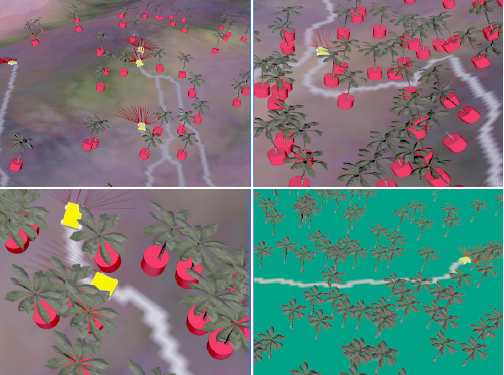
\includegraphics[width=0.33\textwidth,height=5cm]{images/robombeiros2.png}
	    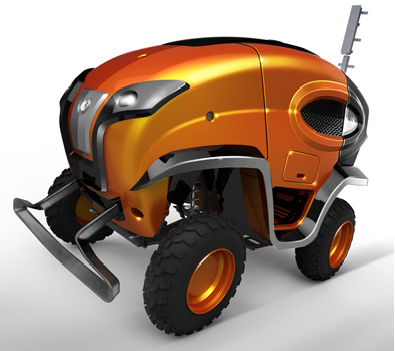
\includegraphics[width=0.33\textwidth,height=5cm]{images/jacto.png}
	    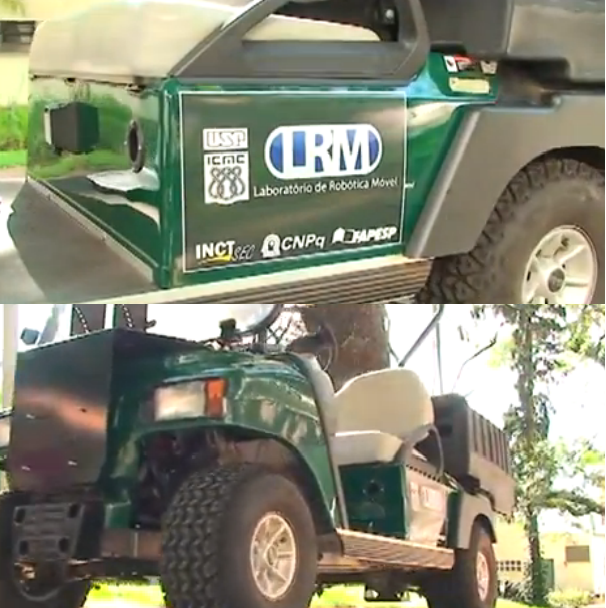
\includegraphics[width=0.33\textwidth,height=5cm]{images/carina_1_stacked.png}
	 	\caption{Simulador RoBombeiros (\textit{esquerda}), 
	 	Jacto JAV (\textit{centro}), CaRINA I (\textit{direita})}
		\fonte{(Jacto S/A, LRM–ICMC/USP)}
	 	\label{fig:um}
 	\end{minipage}
\end{figure}

%2012-10-15 Lido OK


% \section{Contribuições Esperadas}

As principais contribuições acadêmico-científicas esperadas deste trabalho são: 

\begin{enumerate}[i.]

\item adaptação e aperfeiçoamento dos algoritmos para a geração em “tempo real”
de mapas de disparidade, obtendo estes mapas a partir de um par de imagens
capturadas pela câmera estéreo;

\item proposta e desenvolvimento de algoritmos para a obtenção de mapas locais
de navegabilidade com informações espaciais (3D), onde o espaço tridimensional
será dividido em regiões e estas regiões serão identificadas como sendo
navegáveis ou não navegáveis;

\item aperfeiçoamento de técnicas para a navegação baseada no uso de GPS,
bússola e mapas locais de navegabilidade, onde as pesquisas previamente
desenvolvidas para detectar e desviar de obstáculos com o uso de mapas 2D, serão
estendidas a fim de trabalhar com mapa de navegabilidade/ocupação em 3D. Deste
trabalho resultará um sistema com possibilidade de aplicação prática em
importantes tarefas de navegação autônoma, como por exemplo, em sistemas
voltados para aplicações agrícolas e em sistema de combate a incêndio em
florestas, tarefas estas que podem ser perigosas para o ser humano (por exemplo,
exposição prolongada aos produtos químicos de defensivos agrícolas, e
combate/contato direto com fumaça e incêndios).

\end{enumerate}

% \section{Objetivo Geral}
\label{sec:obj_geral}

O objetivo geral deste trabalho é desenvolver um sistema de navegação autônoma baseado
em visão computacional a fim de capacitar um veículo terrestre autônomo a se locomover em
ambientes externos não estruturados, ou seja, em campos com vegetação/plantação e/ou em
florestas pouco densas. O veículo deverá ser capaz de se dirigir até uma localização determinada,
desviando dos obstáculos, percebendo-os de forma autônoma, e escolhendo por meios próprios o
caminho a seguir. O veículo autônomo deverá ter a capacidade de identificar os elementos do terreno
onde irá se deslocar, identificando o chão e os obstáculos, a fim de evitar zonas não transponíveis ou
muito acidentadas. Portanto, o objetivo deste trabalho é desenvolver um sistema de navegação
robusto e seguro voltado à aplicação em veículos autônomos para ambientes externos não
estruturados (ou muito pouco estruturados), baseado no uso de visão computacional realizada
através da captura de imagens estéreo, no uso de mapas de profundidade (mapas de disparidade), e
no uso mapas locais de navegabilidade.

%2010-10-10 REVISAR


%%%\section{Objetivo e Hipótese}

O objetivo deste trabalho é desenvolver um sistema de navegação autônoma baseado
em visão computacional a fim de capacitar um veículo terrestre a se locomover em
ambientes externos não estruturados, ou seja, um campo com vegetação/plantação
e/ou floresta pouco densa. O veículo deverá ser capaz de desviar de obstáculos,
percebendo-os de forma autônoma, e se dirigir até uma localização determinada
escolhendo por meios próprios o caminho a seguir. Deverá ter alguma capacidade
de reconhecer o terreno que irá se deslocar a fim de evitar zonas não
transponíveis ou muito acidentadas.

A informação espacial tridimensional representa mais precisamente o ambiente
onde o veículo autônomo se encontra e por onde deve se locomover, portanto, os
métodos de navegação e representação do ambiente baseados nesta informação
tridimensional são mais abrangentes e menos limitados em relação ao controle e
conhecimento do ambiente.

Tem-se por hipótese então, que algoritmos de navegação planares podem ser
expandidos para o espaço tridimensional se tornando menos limitados e mais
robustos.

%2012-10-15 Revisar

\section{Objetivos Específicos}

Os principais objetivos específicos deste projeto de mestrado, que se apresentam
como um desdobramento do objetivo geral descrito acima, são:

\begin{itemize}

\item Extração de referenciais a partir de um par de câmeras, constituindo um
sistema de visão binocular (estéreo);

\item Propor melhorias nos algoritmos de geração do mapa de disparidade, obtido
a partir das imagens estéreo;

\item Gerar um mapa de navegabilidade local a partir de informações visuais;
%,
%que possa ser adaptado a algoritmos de planejamento e controle de navegação
%autônoma;

\item Desenvolver um mecanismo de navegação autônoma, baseado nas informações de
GPS, Bússola e do Sistema de Visão, capaz de desviar de obstáculos e dirigir o
veículo até um destino determinado de forma robusta e eficiente;

\item Fazer uso dos conhecimentos prévios de trabalhos desenvolvidos no
laboratório e contribuir para a consolidação de tecnologias capazes de atribuir
navegabilidade autônoma a veículos de diversas naturezas para fins práticos;

\item Aplicação e avaliação do sistema de navegação autônoma em um veículo real
em ambiente externo não estruturado.

\end{itemize}

%2012-10-15 Revisar

\section{Objetivo Geral}
\label{sec:obj_geral}

O objetivo geral deste trabalho é desenvolver um sistema de navegação autônoma baseado
em visão computacional a fim de capacitar um veículo terrestre autônomo a se locomover em
ambientes externos não estruturados, ou seja, em campos com vegetação/plantação e/ou em
florestas pouco densas. O veículo deverá ser capaz de se dirigir até uma localização determinada,
desviando dos obstáculos, percebendo-os de forma autônoma, e escolhendo por meios próprios o
caminho a seguir. O veículo autônomo deverá ter a capacidade de identificar os elementos do terreno
onde irá se deslocar, identificando o chão e os obstáculos, a fim de evitar zonas não transponíveis ou
muito acidentadas. Portanto, o objetivo deste trabalho é desenvolver um sistema de navegação
robusto e seguro voltado à aplicação em veículos autônomos para ambientes externos não
estruturados (ou muito pouco estruturados), baseado no uso de visão computacional realizada
através da captura de imagens estéreo, no uso de mapas de profundidade (mapas de disparidade), e
no uso mapas locais de navegabilidade.

%2010-10-10 REVISAR
\section{Justificativa e Aplicações}

%A aplicação de um sistema de visão computacional requer uma boa interpretação da
%imagem, onde a informação contida nela é bastante abrangente, porém de difícil
%acesso. 

Processos mais simples como segmentação, detecção de bordas, e extração de
características locais já são amplamente utilizados em aplicações baseadas em
imagem, mas no caso da navegação robótica em ambientes não estruturados é
necessário o uso de informações de percepção espacial (3D), a fim de identificar
obstáculos e outros elementos que possam prejudicar a navegação do robô.
Com a capacidade de processamento dos computadores atuais, algoritmos mais
complexos e custosos se tornam viáveis, permitindo a concepção de um sistema de
visão computacional mais eficaz. Com o uso de câmeras estéreo associadas com
técnicas para a geração dos mapas de disparidade é possível obter, a partir
deste tipo de câmeras, dados semelhantes aos sensores do tipo
\textit{rangefinder}, baseados em sonar, laser (LIDAR - \textit{Light Detection
And Ranging}) ou infravermelho, porém com uma resolução espacial superior na
ordem de \textit{megapixels}. Além disto, as câmeras são dispositivos de baixo
custo se comparadas, por exemplo, com dispositivos como os sensores a laser de
medida de distância. Até mesmo as câmeras estéreo possuem atualmente um custo
relativamente baixo em relação a estes tipos de sensores pois a princípio são
constituídas a partir de duas câmeras comuns.

Uma das principais motivações deste trabalho advém da possibilidade de uma
aplicação conforme apresentada em um estudo anterior desenvolvido em
\cite{Pessin2008}, onde foi desenvolvido um sistema multiagente de robôs móveis
com a finalidade de combate a incêndios florestais em um ambiente simulado. Os
veículos simulados foram equipados com sonares (ou sensores laser do tipo
LIDAR), bússola e GPS para permitir a navegação autônoma em ambientes externos
não estruturados (\textit{outdoor} e \textit{off-road}). O ambiente adotado foi
tipicamente uma floresta, ou mata não muito densamente ocupada, que permitia o
deslocamento daqueles veículos. Naquele trabalho foi demonstrado com sucesso o
uso de uma Rede Neural Artificial (RNA) treinada para controlar o veículo,
integrando os dados sensoriais e a geração de comandos para os atuadores do
mesmo. Estes veículos robóticos autônomos, denominados de
RoBombeiros\foot{RoBombeiros – Site com material referente ao projeto:
http://sites.google.com/site/pessin}, são capazes de se deslocar em direção ao
foco de incêndio desviando de obstáculos e aproximando do local estimado, onde
devem realizar as ações de combate ao fogo \cite{Pessin2007, Pessin2010}.
Esta abordagem servirá de base e inspiração para o projeto e aplicação do
sistema de controle de navegação que será então desenvolvido, porém será adotado
um sistema de visão computacional como principal informação sensorial e a
utilização de um veículo terrestre real.
% Outra importante aplicação deste trabalho que está sendo proposto é junto a
% aplicações agrícolas: máquinas e implementos agrícolas que possam se deslocar
% pelas plantações para semear, pulverizar defensivos agrícolas, arar a terra, e
% até mesmo realizar a colheita de modo autônomo.

O INCT-SEC e o LRM estabeleceram recentemente uma parceria com uma empresa
brasileira de máquinas agrícolas, a Jacto S/A\foot{Máquinas Agrícolas Jacto S/A
- http://www.jacto.com.br}\foot{Jacto - Pulverizador Autônomo JAV. Vídeo
disponível em: http://www.youtube.com/watch?v=JwTm1kQ2gE0}, cuja sede fica
situada na cidade de Pompéia/SP. A proposta desta cooperação é o desenvolvimento
de soluções robóticas para a automação de veículos agrícolas. Tais veículos
deverão poder atuar em diferentes plantações (por exemplo, café,
\textit{citrus}/laranja e cana-de-açúcar, que são culturas muito difundidas no
estado de São Paulo, e também em outros estados). Testes preliminares foram
realizados pelos membros do Laboratório LRM, demonstrando a viabilidade do uso
de um sistema de visão baseado em câmeras estéreo para uso em aplicações
agrícolas\foot{NAV-AG:
http://www.lrm.icmc.usp.br/?page=projetos\&projeto=navag}.
A \fig{fig:um} apresenta as plataformas robóticas que tem servido como base de
referência para a proposta e desenvolvimento deste projeto:
veículos simulados (RoBombeiros), veículo JAV da Jacto S/A (\textit{Jacto
Autonomous Vehicle}) e veículo automatizado dotado de câmera e atuadores para
navegação autônoma (CaRINA I, desenvolvido junto ao INCT-SEC e ao LRM-ICMC/USP).

\vspace{1cm}

\begin{figure}[!h]
  	\centering
	\begin{minipage}[b]{1.0\linewidth}
	    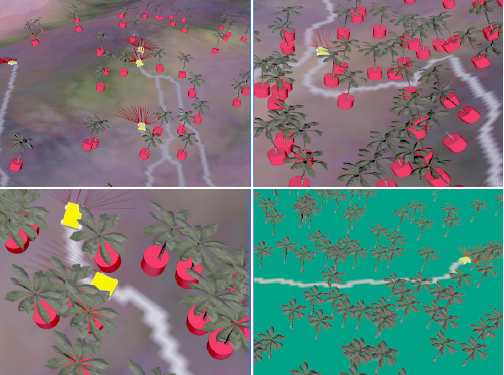
\includegraphics[width=0.33\textwidth,height=5cm]{images/robombeiros2.png}
	    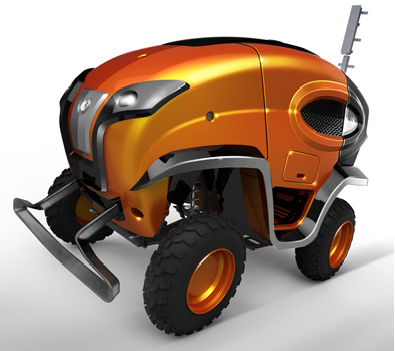
\includegraphics[width=0.33\textwidth,height=5cm]{images/jacto.png}
	    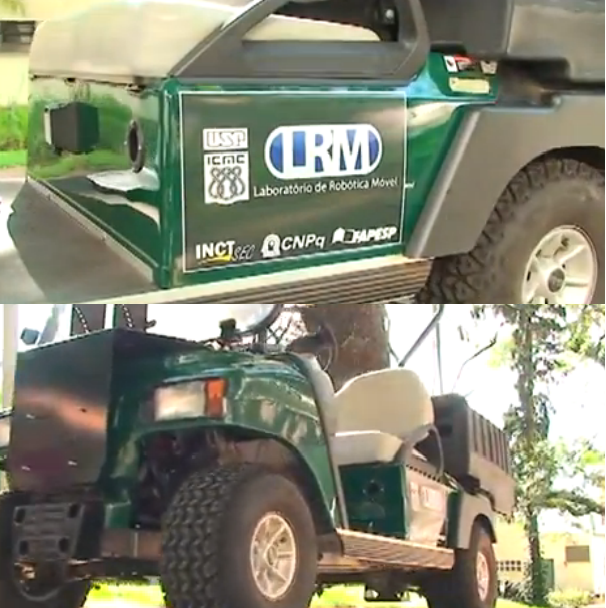
\includegraphics[width=0.33\textwidth,height=5cm]{images/carina_1_stacked.png}
	 	\caption{Simulador RoBombeiros (\textit{esquerda}), 
	 	Jacto JAV (\textit{centro}), CaRINA I (\textit{direita})}
		\fonte{(Jacto S/A, LRM–ICMC/USP)}
	 	\label{fig:um}
 	\end{minipage}
\end{figure}

%2012-10-15 Lido OK


\section{Contribuições Esperadas}

As principais contribuições acadêmico-científicas esperadas deste trabalho são: 

\begin{enumerate}[i.]

\item adaptação e aperfeiçoamento dos algoritmos para a geração em “tempo real”
de mapas de disparidade, obtendo estes mapas a partir de um par de imagens
capturadas pela câmera estéreo;

\item proposta e desenvolvimento de algoritmos para a obtenção de mapas locais
de navegabilidade com informações espaciais (3D), onde o espaço tridimensional
será dividido em regiões e estas regiões serão identificadas como sendo
navegáveis ou não navegáveis;

\item aperfeiçoamento de técnicas para a navegação baseada no uso de GPS,
bússola e mapas locais de navegabilidade, onde as pesquisas previamente
desenvolvidas para detectar e desviar de obstáculos com o uso de mapas 2D, serão
estendidas a fim de trabalhar com mapa de navegabilidade/ocupação em 3D. Deste
trabalho resultará um sistema com possibilidade de aplicação prática em
importantes tarefas de navegação autônoma, como por exemplo, em sistemas
voltados para aplicações agrícolas e em sistema de combate a incêndio em
florestas, tarefas estas que podem ser perigosas para o ser humano (por exemplo,
exposição prolongada aos produtos químicos de defensivos agrícolas, e
combate/contato direto com fumaça e incêndios).

\end{enumerate}


%\chapter{Referencial Teórico}
\chapter{Fundamentação Teórica} 
\label{cap:referencial_teorico}

Um veículo autônomo tem como problemática básica as questões referentes ao
mapeamento, localização e navegação, as quais são fortemente influenciadas pelas
características do ambiente, do problema em questão a ser tratado e da
configuração do robô (sensores e atuadores) \cite{Wolf2009}. Quando se trata
de navegação em ambiente externo, o desconhecimento do ambiente e da sua
dinâmica tornam o mapeamento e localização mais críticos. Em um ambiente
semi-estruturado podemos considerar a existência de algum referencial e impor
alguma restrição, como a existência de caminhos bem definidos e guias, porém
estes devem ser considerados intermitentes, ou seja, o sistema deve ser mais
tolerante à perda momentânea de referenciais. Quando o ambiente não é
estruturado depara-se com a falta de referenciais elementares (linhas, paredes,
trilhas ou vias de deslocamento bem definidas) e com a baixa possibilidade de
imposição de restrições. O desenvolvimento de um sistema autônomo para um
veículo móvel se caracteriza primariamente pelo tratamento destas questões. 

%2012-10-14 Lido OK


%Revisar paragrafo
As pesquisas em veículos terrestres autônomos têm crescido nos últimos anos e já
apresentam aplicações práticas principalmente pela indústria automobilística
para uso em ambiente urbano para o aumento da segurança no uso de automóveis e
na redução de acidentes. Os desenvolvimentos mais recentes podem ser vistos em
\cite{concepts}. 

%Também, a aplicação de veículos terrestres em ambientes
%semi-estruturados ou não estruturados tem chamado a atenção. Este tipo de
%aplicação tem grande interesse econômico em aplicações agrícolas, por exemplo.

Por outro lado, a aplicação de veículos terrestres autônomos em ambientes
semi-estruturados e não estruturados tem também chamado a atenção. Um exemplo
deste tipo deste tipo de utilização são os veículos adotados em aplicações
agrícolas, como já foi citado. 


\section{Mapeamento e Localização}
\label{sec:mapeamento_localizacao}

%A questão do mapeamento e localização é considerado um problema central na
%robótica móvel, 

O mapeamento e localização é uma necessidade recorrente nas aplicações em
robótica móvel, onde a caracterização do veículo como autônomo de fato pode vir
a ser dada essencialmente pela sua capacidade de tratar esta questão. Para que
um robô possa ir de um ponto ao outro do ambiente ele deve conhecer, pelo menos,
a sua localização e a localização do seu ponto de destino. Quando o mapa e a
estrutura do ambiente, assim como a localização do veículo, são desconhecidos a
priori essa questão se torna crítica. Esta necessidade é denominado de SLAM
(\textit{Simultaneous Localization and Mapping}) e é um problema central na
robótica móvel, onde ambas informações dependem uma da outra para serem obtidas. Um
algoritmo proposto para solucionar o SLAM é apresentado em \cite{Thrun2004} que
utiliza uma abordagem probabilística onde as estimativas tando da posição como
do mapeamento são atualizadas uma a partir da outra a medida que dados
sensoriais são coletados.

A visão computacional tem sido aplicada em soluções para o tratamento de SLAM
como a fonte de informação sensorial. Outros equipamentos, como sensor a laser
utilizado em \\\cite{Lategahn2011} e até mesmo sensores inerciais (IMU -
\textit{Inertial Measurement Unit}), como apresentado em \cite{FootSLAM}, são
aplicados e combinados com o propósito de aumentar a acurácia destas medições.
% a localização é estimada pelo onde o erro da estimativa da localização reduz a
% medida que o mapeamento Esse problema é normalmente tratado através de
% abordagens como o SLAM (\textit{Simultaneous Location and Mapping}).
% Uma solução robusta e eficiente para a questão de localização e mapeamento
% simultâneos (SLAM) na prática ainda é desafiadora (\cite{Dissanayake2001}) A
% visão computacional tem sido aplicada em soluções para o tratamento de SLAM ,
% onde uma abordagem recorrente no tratamento da localização e do mapeamento é a
% utilização de visão computacional.
% Porém há uma diversidade de sensores que podem ser integrados com o propósito
% de aumentar a acurácia destas medições, trabalhos recentes como o de
% \cite{FootSLAM} apresenta uma abordagem baseada em sensores inerciais (IMU -
% \textit{Inertial Measurement Unit}).
Entretanto, em ambientes externos (\textit{outdoor}) e extensos a construção de
um mapa global a partir dos dados sensoriais pode não ser viável, comprometendo
a estimação da localização baseada em mapa.
% e a definição da localização em relação a este mapa pode se tornar um problema
% intratável .
Uma solução para determinação da localização em ambientes externos é a obtenção
de coordenadas através do uso do GPS (\textit{Global Positioning System}), que é
baseado na trilateração das distâncias do veículo em relação a uma “constelação”
de satélites deste sistema. Portanto, a posição do veículo e de seu destino pode
ser estimada diretamente (com um certo erro) a partir das informações fornecidas
por um aparelho localizador GPS.



%OSORIO
%> Podia discutir um pouco mais sobre estas questões (expandir esta seção):
%- Dependência da existência de um mapa previamente definido (mapeado pelo robô
%ou não) e do planejamento prévio da rota do robô, ou, navegar no ambiente
%(usualmente não estruturado) sem o uso de um mapa ou de um planejamento prévio
%de rotas (existe o risco de ficar bloqueado, pois possui apenas o conhecimento
%local do ambiente e não realiza um plano global => é bom mostrar que está
%consciente disto).
%- Dependência de um mapa (global) exato e de uma localização exata, ou
%alternativamente, usa um mapa aproximado (local) e usa uma localização também
%aproximada (não muito precisa).
%> São abordagens possíveis e podemos "escolher" entre elas de acordo com o
%problema e requisitos impostos pela aplicação. Obviamente neste trabalho foi
%feita uma escolha (e espero que o leitor se convença que foi uma boa escolha
%dado o contexto)    :)


A localização pode se beneficiar quando há mapas previamente fornecidos, sendo
necessária a localização da posição inicial em relação ao mapa. Os mapas têm
papel importante na tarefa de navegação (seção \ref{sec:navegacao}), tanto
quando fornecidos previamente como quando construídos no momento em que o
veículo se desloca no ambiente. O mapa para navegação geralmente se caracteriza como
local ou global \cite{concepts}. O mapa global provê informações mais
abrangentes sobre o espaço onde o veículo irá se deslocar, principalmente
fornecendo informações sobre obstáculos estáticos e zonas navegáveis
preferenciais, como estradas. Estas informações dos mapas normalmente se
associam a custos, os quais são utilizados pelos algoritmos de planejamento
buscar o melhor caminho. Também, os mapas podem ser representados de forma
métrica (geométrica) e/ou topológica - contendo informações mais detalhadas de o
quê ocupa um determinado espaço (prédio, vegetação, etc.)\cite{Thrun98a}. Já os
mapas locais têm o papel de expressar o ambiente dentro do raio de atuação dos
sensores, ou seja, uma noção localizada próxima ao veículo. Estes mapa local
contém a visão mais atual do ambiente, contemplando obstáculos dinâmicos. A
construção do mapa local pode ser utilizado para agregar informações e atualizar
o mapa global, desta forma, o mapa global se traduz em uma memória do espaço
para o veículo (\fig{fig:map2d}). Quando não há informação prévia que possa ser
utilizada como mapa global é usual uma navegação prévia para o reconhecimento do
ambiente antes que se efetuem tarefas específicas de navegação. Este
reconhecimento inicial pode ser feito de forma autônoma apenas vagando no
ambiente como uma navegação guiada.

\begin{figure}[ht]
%	\centering
	\begin{minipage}[b]{0.9\linewidth}
	    \centering
	    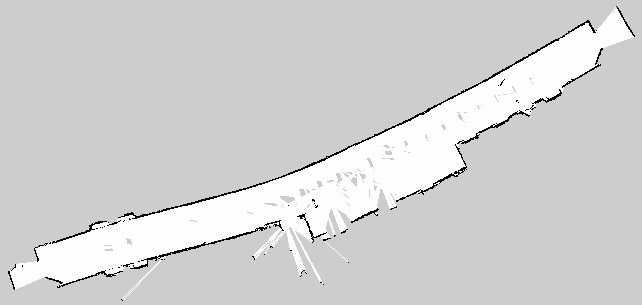
\includegraphics[width=\textwidth,height=6cm]{images/map_2d.jpg}
	 	\caption{Mapa de ocupação planar: Em branco o espaço live, em preto o espaço
	 	ocupado e em cinza o espaço sem informação de ocupação}
		\fonte{www.ros.org (divulgação)}
	 	\label{fig:map2d}
	\end{minipage}
\end{figure}

%2012-10-15 Lido OK (pode ainda ser mais desenvolvido)


\section{Informação Sensorial: Visão Computacional}

Um veículo móvel terrestre se desloca (geometricamente) apoiado sobre um plano
de suporte, ou seja, seus graus de liberdade usualmente podem ser considerados
em duas dimensões. Desta forma, o reconhecimento do chão representa uma
necessidade e se caracteriza um importante desafio ao se considerar um ambiente
externo não estruturado composto por um solo com vegetação. Além da detecção do
chão, é necessária uma certa classificação das regiões deste plano de suporte
(solo) como sendo, por exemplo, uma superfície transitável ou não transitável:
devido à presença de vegetação, obstáculos, buracos e demais impedimentos.
Os sensores típicos, como sonares e lasers, não apresentam dados muito adequados
para viabilizar essa classificação, uma vez que o sonar possui uma limitação de
alcance e de precisão e o sensor laser de 1 feixe é capaz apenas de analisar uma
seção planar do espaço tridimensional (além de ter um custo muito elevado para
certas aplicações). As câmeras de vídeo são mais adequadas para capturar tais
informações que caracterizam o ambiente, principalmente, se forem usadas câmeras
estéreo, das quais é possível extrair uma informação de profundidade dos
elementos da cena capturada. A utilização de câmeras de vídeo demandam algumas
tarefas elementares, como o ajuste de foco, a utilização de lentes adequadas ao
ângulo de visão necessário e uma devida calibragem. A calibragem das câmeras é
um processo fundamental para se obter um sistema de visão computacional com
representação tridimensional a partir de um par de câmeras independentes
(binocular). Neste processo são calculados (estimados) os parâmetros internos e
externos de cada câmera. Estes parâmetros são essenciais para a reconstrução
tridimensional a partir das imagens capturadas pela câmera estéreo
\cite{Faugeras1993}.

A estimação dos parâmetros internos (intrínsecos) consiste em se obter a
distância focal e o ponto central da imagem, que por questões de alinhamento
entre lentes e sensor pode não ser o pixel central da imagem, influenciando
fortemente os demais processos de estimação \cite{WilsonShafer1994}. Estes
dois parâmetros definem como a imagem é formada por uma câmera estilo
estenopeica (\textit{pin-hole}) e a sua projeção perspectiva. Outros parâmetros
também internos, não associados com o modelo de projeção e sim com as
características físicas das lentes utilizadas, também são estimados no processo
de calibragem. No caso das câmeras de vídeo existe a necessidade de utilização
de lentes, tanto para reduzir a imagem a ser projetada no sensor (filme/CCD)
como para aproximá-las. As lentes comumente são estruturas com curvatura
esférica, característica esta que provoca distorções óticas na imagem projetada.
Estes efeitos são chamados de distorções radiais, produzindo imagens com
demonstrado na \fig{fig:distortions}, nos casos, onde esta distorção pode ser em
forma de “barril” (\textit{barrel}) ou “almofada” (\textit{pincushion})
\cite{Weng1992}.

% (\fig{fig:int_param}).
As distorções óticas influenciam fortemente de forma negativa o processo de
correspondência entre as imagens para extrair a informação tridimensional, sendo
grande fonte de ruído quando não corrigidas. É interessante notar que,
matematicamente, o processo de correção das distorções óticas se baseia na
curvatura esférica da lente, porém as lentes são formadas por uma composição de
várias camadas com curvaturas diferentes (\fig{fig:lens}), que ainda podem
apresentar defeitos no processo de fabricação. Portanto, o modelo matemático
utilizado na correção é sempre uma aproximação global do aparato ótico, fonte
por si só de imprecisão \cite{WilsonShafer1994}.

%Existem ainda outros
%parâmetros que podem ser considerados, porém, estes estão associados a questões
%técnicas da forma de aquisição da imagem e não à formação da imagem propriamente
%dita, portanto são subjetivas ao aparato utilizado sendo necessárias ou não, a
%exemplo, os problemas referentes ao entrelaçamento e varredura da imagem.

% \begin{figure}[ht]
% 	\centering
% 	\begin{minipage}[b]{0.3\linewidth}
% 	    \centering
% 	    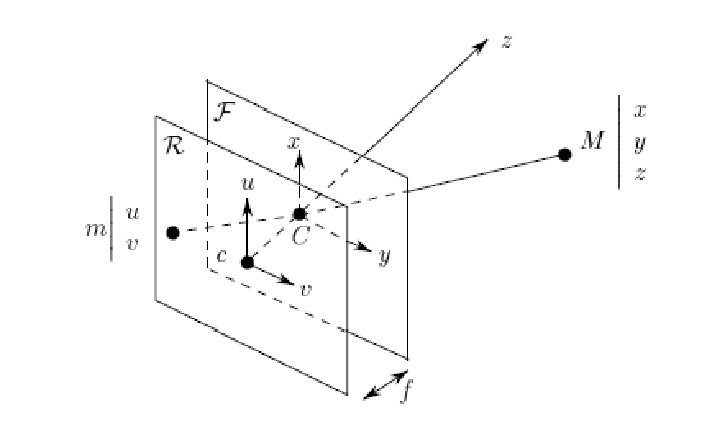
\includegraphics[width=\textwidth]{images/int_param.png}
% 	 	\caption{Ponto central e distância focal}
% 		\fonte{(\cite{Faugeras1993})}
% 	 	\label{fig:int_param}
% 	\end{minipage}
% 	\hspace{0.1cm}
% 	\begin{minipage}[b]{0.3\linewidth}
% 	    \centering
% 	    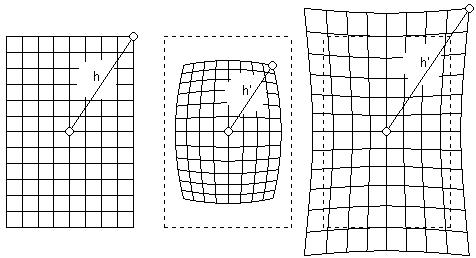
\includegraphics[width=\textwidth]{images/distortions.png}
% 	 	\caption{Distorções óticas}
% 	 	\label{fig:distortions}
% 	\end{minipage}
% 	\hspace{0.1cm}
% 	\begin{minipage}[b]{0.3\linewidth}
% 		\centering
% 	    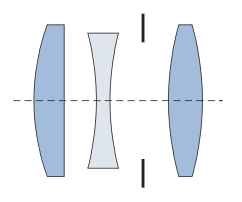
\includegraphics[width=\textwidth,height=3cm]{images/lens.png}
% 	 	\caption{Exemplo de composição ótica}
% 	 	\label{fig:lens}
% 	\end{minipage}
% \end{figure}

\begin{figure}[ht]
	\centering
	\hspace{0.1cm}
	\begin{minipage}[b]{0.45\linewidth}
	    \centering
	    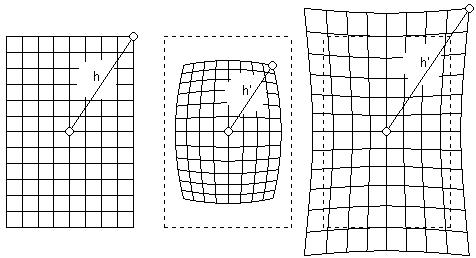
\includegraphics[width=\textwidth]{images/distortions.png}
	 	\caption{Distorções óticas: sem distorção (\textit{esquerda}), 
	 	distorção tipo “barril” (\textif{centro}), 
	 	distorção tipo “almofada” (\textit{direita}).}
	 	\label{fig:distortions}
	\end{minipage}
	\hspace{0.1cm}
	\begin{minipage}[b]{0.45\linewidth}
		\centering
	    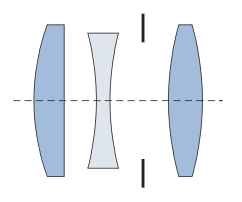
\includegraphics[width=\textwidth,height=4cm]{images/lens.png}
	 	\caption{Exemplo de composição ótica de lentes.}
	 	\label{fig:lens}
	\end{minipage}
\end{figure}


De posse dos parâmetros internos associados às distorções é necessário um
pré-processamento para a sua correção que ao ser aplicado produz uma imagem mais
própria para os algoritmos de correspondência que formarão a imagem
tridimensional. Os parâmetros internos são também chamados de parâmetros do
modelo, isto é, como a imagem é formada. Um outro modelo de câmera geralmente
associado a veículos móveis são as câmeras omnidirecionais, capazes de produzir
uma imagem em 360 graus, útil para veículos com esse grau de liberdade de
movimentos. A calibragem deste tipo de câmera é ainda mais complexa. O segundo
conjunto de parâmetros são os parâmetros externos (extrínsecos), também chamados
de parâmetros de pose. Este conjunto diz respeito à posição da câmera em relação
ao ambiente, no caso, a um sistema de coordenadas referencial. Estes são os
principais parâmetros para a reconstrução tridimensional, pois são utilizados
para se chegar a uma correspondência entre os pixeis de cada uma das duas
imagens. Esta correspondência entre os pontos é obtida pelos princípios da
geometria epipolar (\fig{fig:epipolar}) \cite{Faugeras1993}. De posse dessa
correspondência, a partir do deslocamento destes pontos (disparidade) e um
processo de triangulação, pode ser construída uma representação tridimensional
em um mapa de profundidade. Fundamentalmente, são determinados os planos
formados pelos pontos em comum em cada imagem (referenciais obtidos pela
calibragem) e o ponto central de cada imagem. Esses planos no espaço (ambiente)
são coincidentes, ou seja, o mesmo plano de corte. Esta projeção do plano em
cada imagem definem retas, chamadas retas epipolares. Desta forma é possível
fazer a correspondência dos demais pontos (não referenciais). Este alinhamento
das imagens é chamado de retificação \cite{Fusiello2000}, como pode ser visto
na \fig{fig:rectification}. Pela geometria epipolar todos os planos formados
pelos pontos referenciais serão concorrentes e as suas intersecções se dão em
uma reta em comum, chamada linha base. Esta linha base determina o alcance da
visão (profundidade).

Em um estudo anterior realizado por Klaser \cite{Klaser2007}, em seu trabalho
de conclusão de graduação (TCC), foi aplicada visão tridimensional para
monitorar experimentos de laboratório utilizando como processo de calibragem o
método de Tsai \cite{Tsai1987}. Naquele trabalho, onde as duas câmeras podiam
ser posicionadas em relação ao ambiente com uma certa liberdade observando-se
alguns critérios, foi possível verificar que um conjunto de referenciais capazes
de descrever os três planos ortogonais do espaço tridimensional produziam uma
calibragem bastante precisa. Para isso, foi utilizado um molde semelhante ao
canto de uma sala contendo pelo menos três pontos referenciais em cada parede e
no chão (\fig{fig:bioview}). Uma vantagem do método de Tsai é que o referencial
para a calibragem é dado informando sua posição na imagem e sua posição real no
ambiente, sendo a posição real dada de forma relativa a um sistema de
coordenadas referencial no espaço. Com isso, ao extrair a informação
tridimensional de um ponto pelo processo de triangulação a partir da calibragem
do par estéreo, a informação resultante contém as coordenadas espaciais do ponto
na unidade de medida adotada. Desta forma, é possível saber a posição real de um
determinado ponto, podendo ser extraída uma nuvem de pontos 3D do ambiente
(\textit{3D point cloud}). Porém, para se obter as coordenadas tridimensionais
de um determinado ponto no espaço é necessário saber onde esse ponto se encontra
em cada imagem \cite{MundyZisserman1994}.
Isto não é trivial, mas é possível utilizar métodos de detecção e casamento
(\textit{matching}) de características (\textit{features}) das imagens para
buscar a correspondência, como por exemplo, o método SIFT
(\textit{Scale-Invariant Feature Transform}) \cite{Lowe1999} e o método SURF
(\textit{Speeded Up Robust Features}) \cite{Bay2008}.
% Uma abordagem baseada neste princípio em que, a partir de duas poses da mesma
% cena, se extrai uma terceira coordenada tendo por base uma calibragem das
% câmeras e um processo de correlação global dos pixeis, é chamada de mapa de
% disparidade. Este processo é computacionalmente custoso e existem diversas
% técnicas para a sua implementação.
Uma abordagem para extrair a terceira coordenada espacial tendo por base duas
imagens da mesma cena em poses diferentes e a devida calibragem é chamada de
disparidade \cite{Qian97binoculardisparity}. Este processo é computacionalmente
custoso e existem diversas técnicas para a sua implementação.

\begin{figure}[ht]
	\begin{minipage}[b]{0.3\linewidth}
	    \centering
	    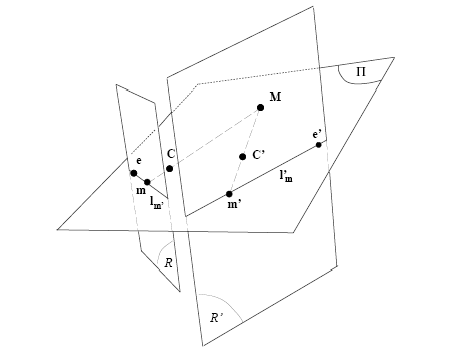
\includegraphics[width=\textwidth]{images/epipolar.png}
	 	\caption{Geometria epipolar}
		\fonte{\cite{Faugeras1993}}
	 	\label{fig:epipolar}
	\end{minipage}
	\hspace{0.1cm}
	\begin{minipage}[b]{0.3\linewidth}
	    \centering
	    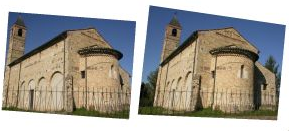
\includegraphics[width=\textwidth,height=4cm]{images/rectification.png}
	 	\caption{Retificação }
		\fonte{Andrea Fusiello}
	 	\label{fig:rectification}
	\end{minipage}
	\hspace{0.1cm}
	\begin{minipage}[b]{0.3\linewidth}
		\centering
	    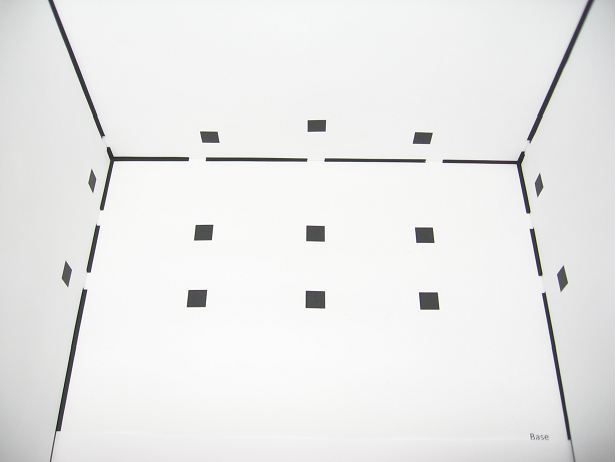
\includegraphics[width=\textwidth,height=4cm]{images/bioview.png}
	 	\caption{Calibragem com referenciais fixos}
		\fonte{\cite{Klaser2007}}
	 	\label{fig:bioview}
	\end{minipage}
\end{figure}

\vspace{0.5cm}


%OSORIO
%> Podia acrescentar uma breve seção sobre GPS:
%2.3 Sensores: Localização e Orientação
%descrevendo sobre a posição (GPS) e orientação (bússola), do veículo e de seu
% destino.
%> O parágrafo abaixo já é uma espécie de "resumo e consolidação" do que foi
%apresentado nas seções anteriores.

Portanto, neste trabalho serão adotados os sensores do tipo GPS e Bússola
(posição e orientação) para localização e câmeras estéreo para a extração de
mapas locais. Estes mapas descreverão o ambiente e os obstáculos através de uma
representação espacial (3D) na qual se encontra o veículo robótico autônomo. A
câmera estéreo irá fornecer um mapa de navegabilidade local composto por
informações obtidas a partir do mapa de disparidade que será descrito a seguir.

%OSORIO
%> Senti falta de uma noção mais geral sobre como passamos da parte de visão
% computacional estéreo para os mapas locais (mapa 3D - cloud of points, mapa local, mapa de navegabilidade). 
% Mapa de disparidade já entra em um conceito específico...
%> Talvez pudesse ter citado o trabalho do Caio (mestrado) e do Patrick
% (mestrado) que tem bons exemplos de mapas (com figuras)  :)


% 2012-10-13 lido OK


\section{Mapas de Disparidade}
\label{sec:mapas_disparidade}

Os mapas de disparidade se tornaram uma ferramenta bastante utilizada para a
percepção tridimensional. Para robôs móveis autônomos os mapas de disparidade
são muito úteis, principalmente na detecção e desvio de obstáculos. O veículo
pode extrair uma informação de profundidade que servirá como parâmetro para a
navegação, por exemplo, uma região frontal de maior profundidade pode
representar um caminho sem obstáculos, livre de objetos e elementos localizados
em frente a câmera. Atualmente, a implementação direta em hardware dos
algoritmos de cálculo do mapa de disparidade a partir de um par de imagens
(câmera estéreo) permite a aplicação em tempo real e de forma embarcada
(\fig{fig:stoc_on_chip}) \cite{Khaleghi2008}.

A ideia fundamental do mapa de disparidade é fornecer uma informação de
profundidade relativa, mapeada diretamente na imagem bidimensional a partir do
valor do pixel. Usualmente são utilizadas imagens em tons de cinza (8
\textit{bits}), fornecendo então até 255 níveis de profundidade. Na
\fig{fig:tsukuba}, o mapa de disparidade está representando os obstáculos mais
próximos por tons mais claros e os obstáculos mais distantes por tons mais
escuros. Desta forma, os pixeis da imagem passam a representar no lugar da
informação de cor ou luminosidade uma informação de profundidade sobre os
elementos da cena. Os dispositivos sensores que fornecem uma imagem colorida
juntamente com o mapa de disparidade têm sido denominados de dispositivos RGB-D
(Imagem RGB + \textit{Depth}/mapa de disparidade). O sensor Kinect da
Microsoft\foot{Microsoft Kinect - http://www.xbox.com/en-us/kinect} fornece
imagens RGB-D com uma precisão de 2047 níveis de profundidade. Uma avaliação da
qualidade do mapa de disparidade produzido pelo Kinect \cite{Khoshelham2012}
mostrou que a relação entre o nível de profundidade e distância não é linear,
onde a distância real dos objetos é gradualmente maior do que a distância
estimada a medida que se afastam da câmera. O Kinect é utilizado atualmente como
base de comparação pois é uma aplicação em larga escala comercial desta técnica
e produz resultados práticos satisfatórios.

\vspace{0.5cm}
\begin{figure}[h!!!]
	\centering
	\begin{minipage}[b]{0.4\linewidth}
	    \centering
	    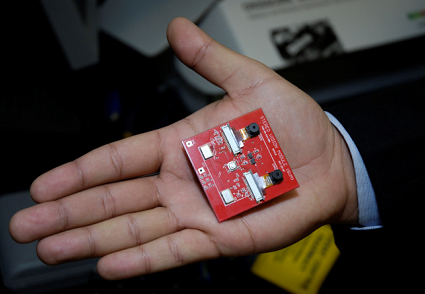
\includegraphics[width=\textwidth,height=4.5cm]{images/stoc_on_chip.png}
	 	\caption{Sistema de visão tridimensional
embarcado baseado em mapa de disparidade}
		\fonte{\cite{Khaleghi2008}}
	 	\label{fig:stoc_on_chip}
	\end{minipage}
	\hspace{0.1cm}
	\begin{minipage}[b]{0.55\linewidth}
	    \centering
	 	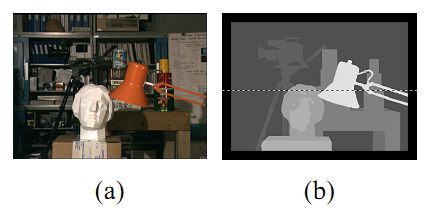
\includegraphics[width=\textwidth,height=4.5cm]{images/tsukuba.png}
	 	\caption{Estéreo: \textbf{(a)} imagem RGB \\ \textbf{(b)} disparidade referencial}
		\fonte{University of Tsukuba}
	 	\label{fig:tsukuba}
	\end{minipage}
\end{figure}

%Porém, essa não linearidade não é um artefato
%que resulta propriamente daquela implementação, 
%ela advém do fato de o mapa ser
%gerado a partir de imagens que são formadas pela projeção perspectiva que 
%inerentemente produz esse efeito (\textit{foreshortening}).

Em sistemas onde as câmeras são estacionárias (fixas em um local), como na
aplicação tradicional do Kinect, técnicas de extração e supressão do fundo podem
ser utilizadas para aumentar a robustez do método \cite{Ivanov2000}. No caso das
aplicações em robótica móvel, as câmeras estão em constante movimento
potencializando estes efeitos negativos, fazendo-se necessário outros métodos
para minimizar estes efeitos. Outra característica a ser apontada em relação ao
Kinect é sua inviabilidade de uso no ambiente externo, ou seja, com iluminação
natural - isto se deve ao fato da tecnologia empregada se basear em luz
estruturada e requer iluminação artificial (infra-vermelho) a qual sofre
interferência na presença de luz solar. Em ambiente externo são utilizadas
câmeras convencionais, onde o conjunto estéreo pode ser constituído tanto por
câmeras independentes permitindo maior versatilidade de poses como no uso de
câmeras do tipo STOC (\textit{STereo On a Chip}) que são mais estáveis em
relação à manutenção da calibragem.

%Em ambiente externo são utilizadas câmeras convencionais
%porém geralmente o uso de câmeras estéreo tipo STOC (\textit{STereo On a Chip})
%são um tipo de aplicação por serem mais estáveis em relação à manutenção da
%calibragem devido a vibrações.

%Fig. 2.7: Sistema de visão tridimensional
%embarcado baseado em mapa de disparidade
%Fonte: 
%Fig. 2.8: a) Imagem RGB; b) Mapa de disparidade Fonte: University of Tsukuba 

O mapa de disparidade provê uma percepção espacial que representa os elementos
da cena em um espaço tridimensional, fornecendo assim, uma fonte muito rica de
informações sobre a cena. A partir destas informações pode ser possível então
definir a trajetória do veículo de modo a desviar dos obstáculos que se
encontram a sua frente ao mesmo tempo em que este se locomove em direção ao seu
destino. Este processo é denominado de navegação robótica e será detalhado a
seguir.


%%2012-10-14 Lido OK

\section{Navegação}
\label{sec:navegacao}

A navegação em campo aberto se torna um problema de tomada de decisões difícil,
devido à ausência de um mapa global atualizado, a falta de referenciais locais e
o excesso de ruído dos sensores, que produzem pouca informação válida para o
sistema. Apesar do veículo estar buscando um destino preestabelecido, dirigir-se
sempre em linha reta pode não ser a melhor decisão, ou mesmo impossível. Além
disto, a indicação da posição atual (localização) pode não ser totalmente
confiável.

Ainda que se utilize GPS, esse sistema apresenta erro na localização exata
(usualmente com um erro médio de cerca de 5
metros\foot{http://en.wikipedia.org/wiki/Error\_analysis\_for\_the\_Global\_Positioning\_System}),
pois considera-se também o fato de que o veículo não tem uma estrada ou via como
referência (ambiente não estruturado). Já no caso de dispositivos como o
odômetro, utilizados para manter um controle da localização por
\textit{dead-reckoning} \cite{Dudekbook}, a confiabilidade é ainda menor pois
há grande tendência de discrepância uma vez que o erro é cumulativo. Estas
discrepâncias podem ser resultantes de derrapagens das rodas, erros de estimação
da real distância percorrida ou mesmo das alterações involuntárias de direção do
veículo. Uma possível melhoria da precisão do GPS pode ser conseguida usando um
sistema de correção DGPS (GPS diferencial), onde antenas em solo são utilizadas
para aumentar a precisão do local estimado pelos sinais dos satélites. No
entanto, nem sempre este tipo de abordagem é possível pela falta desta
infraestrutura no local desejado, além de possuir um custo bem mais elevado em
relação a abordagem tradicional. No Brasil, o IBGE\foot{IBGE –
http://www.ibge.gov.br} disponibiliza serviços de posicionamento de precisão
através da RBMC\foot{RBMC –
http://www.ibge.gov.br/home/geociencias/geodesia/rbmc/rbmc.shtm} (Rede
Brasileira de Monitoramento Contínuo). O GPS tradicional possui um erro médio
usual entre 5 a 10 metros da posição estimada informada em relação a posição
real, enquanto um DGPS pode reduzir este erro médio para menos de 1 metro
(aproximadamente 50 cm).

É interessante observar que em aplicações de GPS em roteiros rodoviários (e
urbanos) a existência de um mapa local permite um certo ajuste de coerência que
visualmente dá a impressão de uma maior precisão, porém em campo aberto esta
abordagem não é possível. Existe inclusive um “jogo”, denominado de
GeoCaching\foot{GeoCaching Game:
http://www.geocaching.com/guide/default.aspx}, inspirado nesta ideia de
navegação baseada em GPS, onde o usuário deve encontrar um ponto de destino
usando como informação apenas as coordenadas GPS disponíveis, logo, a
dificuldade é exatamente a imprecisão. 

O algoritmo básico de navegação de um veículo autônomo pode se basear em um
princípio estratégico similar ao utilizado por uma pessoa portadora de
deficiência visual, ou seja, passos controlados e o constante monitoramento do
ambiente ao seu redor. Uma pessoa consegue achar, de modo intuitivo e racional,
um caminho em direção a um determinado destino e evitar colisões com obstáculos
em seu caminho. No caso de um veículo autônomo, este não possui essa capacidade
intrínseca de navegação e desvio de obstáculos, devendo ser dotado de algum
recurso computacional e/ou físico para tal. Existem diversos algoritmos
clássicos de estratégia de navegação, como por exemplo, o algoritmo do
\textit{bug} \cite{Choset2005} e suas variantes \cite{Taylor2009}, que se
baseiam na detecção de bordas (obstáculos) e executam a locomoção aproximando-se
a elas e fazendo o seu contorno.


\subsection{Planejamento}

A operação de navegação requer um planejamento, este planejamento pode ser
categorizado como local ou global. No planejamento global há a necessidade de
que o ambiente seja previamente conhecido através da representação de um mapa
global (geralmente estático), enquanto que o planejamento local se baseia apenas
na posição onde o robô se encontra e no alcance dos seus sensores. As
metodologias de planejamento podem ser agrupadas em quatro categorias
principais: gráficas, clássicas, heurísticas e de campo potencial. As
metodologias baseadas em campos potenciais são soluções elegantes que se baseiam
em forças de repulsão aos obstáculos e forças de atração ao destino, podendo ser
aplicado para o planejamento local. Porém, de acordo com o tipo de ambiente em
que o robô se encontra podem apresentar problemas relacionados a mínimos locais
devido a forças de repulsão demasiadas que inibem o movimento do robô. Em
ambientes abertos e com poucos obstáculos os campos potenciais são uma abordagem
largamente adotada. O VFH (\textit{Vector Field Histogram})
\cite{Borenstein1991} aplica esta ideia e teve como proposta inicial a tentativa
de evitar os mínimos locais, dentro do que for possível com relação as
informações sensoriais disponíveis.

%proposta inicial a solução
%da questão dos mínimos locais.

%Uma técnica em destaque na abordagem de campos potenciais é
%o VFH (\textit{Vector Field Histogram}) (\cite{Borenstein1991}), que soluciona
%diversos problemas associados a este tipo de abordagem.

O método VFH foi projetado para ser utilizado em tempo real a partir dos dados
dos sensores, gerando um histograma (\fig{fig:vfh}) onde os picos representam a
proximidade dos objetos em relação ao veículo e os vales os espaços livres.
Idealizado para ser utilizado com sensores do tipo sonar, leva em conta as
questões inerentes a ruídos próprios desta classe de sensor e as características
cinemáticas do veículo.

%, sendo base para
%outros métodos que utilizam esta abordagem de campo potencial/campo de força.

\vspace{0.5cm}
\begin{figure}[ht]
	\centering
	\begin{minipage}[b]{1\linewidth}
	    \centering
	    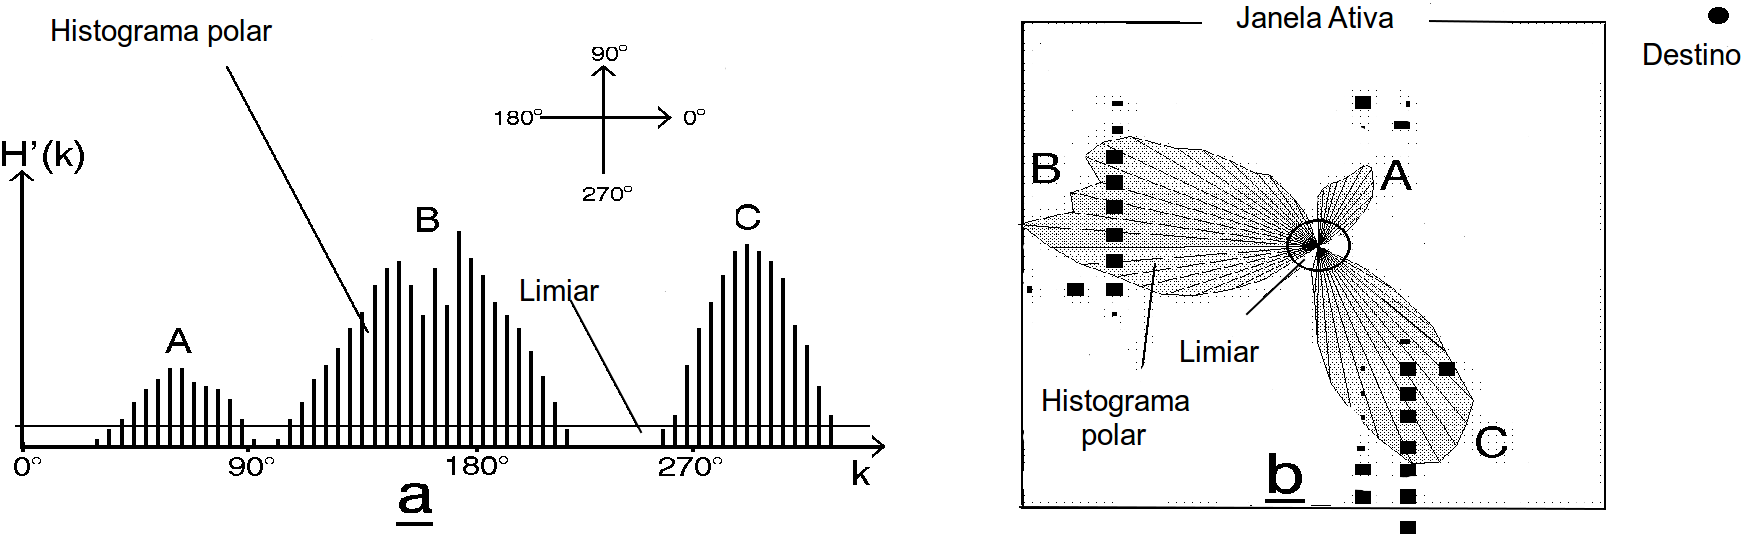
\includegraphics[width=\textwidth,height=7cm]{images/vfh_horiz.png}
	 	\caption{VFH - \textbf{(\underline{a})} Gráfico do histograma, 
	 	onde H'(k) representam as forças de repulsão aos obstáculos nas direções k.\\
	 	\textbf{(\underline{b})} Representação espacial em relação aos 
	 	obstáculos (retângulos em preto) - A área circulada representa a posição do robô.}
		\fonte{adaptado de: \cite{Borenstein1991}}
	 	\label{fig:vfh}
	\end{minipage}
\end{figure}


%Para o planejamento global, de posse de uma mapa convertido em custos 

Enquanto o VFH tem um comportamento mais reativo, em um cenário onde um mapa
global mesmo que incompleto é fornecido pode ser adotado um método deliberativo
para o planejamento da trajetória até um destino.

Os algoritmos de geração de trajetória baseados em amostras tem sido adotado em
robótica móvel com maior ênfase principalmente pela aplicabilidade prática, este
tipo de abordagem leva em consideração a cinemática do veículo gerando
trajetórias realistas com custo computacional baixo \cite{ompl}.

Estes métodos inicialmente constroem um grafo baseado em amostras de trajetórias
que o veículo pode executar, onde geralmente se limita a algumas manobras afim
de reduzir as ramificações do grafo \cite{topologic}. Após esta etapa pode ser
executado um método gráfico de busca por um caminho de menor custo baseado no
menor caminho e proximidade de obstáculos \fig{fig:sbpl}.

\begin{figure}[ht]
	%\hspace{0.1cm}
	\centering
	\begin{minipage}[b]{1\linewidth}
	    \centering
	 	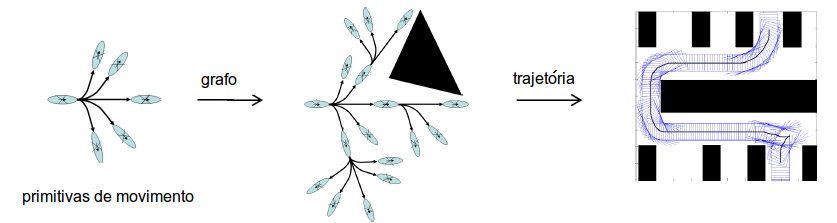
\includegraphics[width=\textwidth,height=5cm]{images/sbpl.png}
	 	\caption{Planejamento de trajetória por amostras}
	 	\fonte{adaptado de: www.ros.org}
	 	\label{fig:sbpl}
	\end{minipage}
\end{figure}
%No trabalho de \cite{} foi utlilizada a biblioteca SBPL
%(\textit{Search-based Planning Library}) 

%Os métodos heurísticos
% baseados em amostra 

\subsection{Controle}

O controle de navegação de um robô móvel pode ser classificado basicamente como
reativo, deliberativo ou híbrido \cite{Wolf2009}, podendo ser estruturada de
forma hierárquica; um caso particular de arquitetura híbrida em camadas. No
projeto COHBRA \cite{Heinen2002}, foi utilizada a abordagem híbrida em camadas
para a criação de um sistema de controle para robôs móveis. Esta abordagem
híbrida permite ao sistema de controle planejar e executar um plano de uma
trajetória (camada deliberativa) ao mesmo tempo em que detecta a presença e
desvia de obstáculos que não foram previamente mapeados (camada reativa). As
técnicas aplicada na elaboração do sistema de controle podem ser baseadas em
Máquinas de Estados Finitos (FSM – \textit{Finite State Machines}), Sistemas
Especialistas e/ou Sistemas Nebulosos (FIS - \textit{Fuzzy Inference Systems}),
Redes Neurais Artificiais (RNA), ou mesmo, uma combinação destes em diversas
camadas. 

As RNAs são consideradas sistemas "caixa-preta": após o treinamento da RNA os
pesos sinápticos associados a cada neurônio (por exemplo, perceptron) não têm
propriamente um “significado”, somente valores numéricos que representam o
conhecimento adquirido. A sua capacidade de generalização torna-a tolerante a
ruídos e permite a aplicação principalmente quando não se consegue estruturar
totalmente o problema a partir de regras bem definidas. É uma técnica
extremamente plástica, podendo ser aplicada a diversas classes de problemas. O
sistema SEVA3D \cite{Heinen2007} se baseou no aprendizado neural de um FSM
(Finite-State Machine) para fazer o controle de navegação do veículo, já no
simulador RoBombeiros \cite{Pessin2008}, adotou-se uma RNA para este fim
(\fig{fig:ann_pesin}).

\vspace{0.5cm}
\begin{figure}[ht]
	%\hspace{0.1cm}
	\centering
	\begin{minipage}[b]{0.6\linewidth}
	    \centering
	 	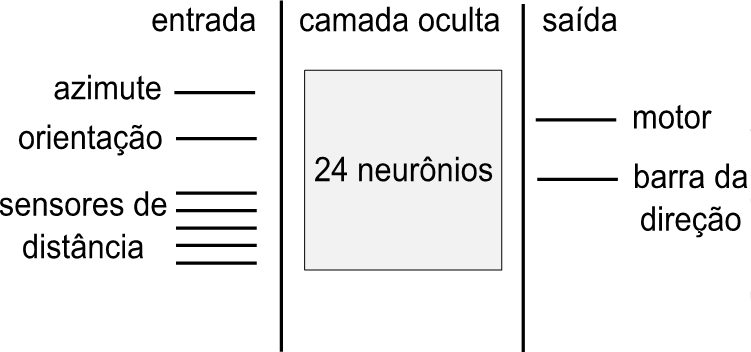
\includegraphics[width=\textwidth,height=5cm]{images/ann_pesin.png}
	 	\caption{Arquitetura da RNA no simulador RoBombeiros}
	 	\label{fig:ann_pesin}
	\end{minipage}
\end{figure}


%OSORIO
%> Podia detalhar um pouco mais sobre o Robombeiros aqui... se não for detalhar
% mais adiante, seria bom ser mais "didático" pois nem todos da banca sabem do
% que se trata e como funciona (assim como os futuros leitores deste texto)

No caso dos RoBombeiros, o controle pela rede neural era de um comportamento
basicamente reativo, onde ao mesmo tempo que direcionava o veículo para o
destino gerava comandos de desvio na presença de obstáculos próximos. Nesta rede
neural foi projetado como entrada a orientação do veículo dada por uma bússola e
a sua orientação em relação ao ponto de destino calculada pelas posições de GPS,
assim como informações sensoriais de distâncias de objetos presentes no raio de
ação do sensor laser utilizado. Desta forma a rede neural foi treinada para
gerar comandos de aceleração e esterçamento que controlavam a navegação do
veículo autônomo.

%2012-10-15 Lido OK

\section{Espaço Tridimensional}

É notório verificar que as abordagens de navegação autônoma de veículos
terrestres mais usuais se baseiam em grande parte na restrição de uma visão
planar do ambiente, ou seja, um mundo plano. De fato, isto simplifica os modelos
e é uma abordagem consciente das suas limitações em relação à fidelidade de
representação do mundo real. Para ambientes controlados e até mesmo problemas
reais restritos a abordagem planar é bem sucedida. Já a abordagem tridimensional
é mais geral do que a abordagem planar pois descreve o espaço em todas as suas
reais dimensões. Portanto, ela contempla o caso planar como caso particular. Por
outro lado, inerentemente o custo computacional associado se torna mais elevado
devido aos aumento da complexidade e dimensionalidade dos modelos.

No que diz respeito a recursos computacionais, a computação embarcada atual já
viabiliza diversas aplicações onde modelos mais completos e complexos se tornam
praticáveis. Isto se traduz não só em maior realismo quando se trata da relação
com o utilizador do sistema como maior precisão devido aos modelos mais
completos. É neste sentido que as abordagens tridimensionais, no que diz
respeito à percepção do ambiente onde se inserem os robôs móveis, têm sido
buscadas pela comunidade científica atualmente.

A visão estéreo se insere neste contexto e é uma ferramenta para a extração da
informação tridimensional do ambiente. Os sensores laser tem desempenhado papel
importante na construção destes algoritmos por produzirem dados precisos a um
baixo custo computacional pois não há a necessidade de transformação do dado
capturado, como ocorre no caso das câmeras. Por outro lado são sensores
extremamente especializados, com características que por vezes limitam sua
aplicação real - são equipamentos sensíveis e geralmente não podem ser cobertos
por uma proteção, por exemplo. Câmeras de vídeo são de uso geral sendo
largamente utilizadas em diversas aplicações.

Conforme descrito na Seção \ref{sec:mapas_disparidade}, a partir de um conjunto
de câmeras através de uma visão estéreo é possível extrair informação visual do
espaço tridimensional do ambiente. Tais dados são convertidos em nuvens de
pontos (\fig{fig:nuvem_pontos}), e assim como para os sensores laser, os métodos
aplicados à interpretação e classificação se dão a partir destes pontos. Uma
nuvem de pontos nada mais é do que um conjunto de pontos no espaço sem
informação de correlação, apenas os dados de pontos no espaço. No caso das
câmeras, a informação cromática pode ainda ser agregada a estes pontos. Em
geral, as nuvens de pontos são classificadas de acordo com a sua densidade,
podendo ser esparsa ou densa. As câmeras apresentam outra vantagem por não só
produzirem pontos tridimensionais como provêem uma imagem do cenário, onde por
métodos de processamento de imagens e de visão computacional é possível extrair
diversas características que permitem uma interpretação da cena não
necessariamente tridimensional.

\vspace{0.5cm}

\begin{figure}[ht]
%	\centering
	\begin{minipage}[b]{0.33\linewidth}
	    \centering
	    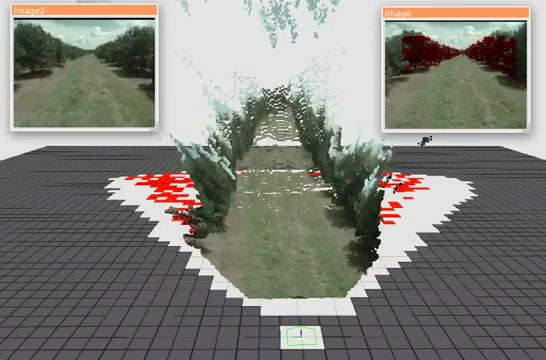
\includegraphics[width=\textwidth,height=4cm]{images/nuvem_pontos_caio.jpg}
	 	\caption{Nuvem de pontos a partir de câmera estéreo}
		\fonte{LRM (divulgação)}
	 	\label{fig:nuvem_pontos}
	\end{minipage}
	\begin{minipage}[b]{0.33\linewidth}
	    \centering
	    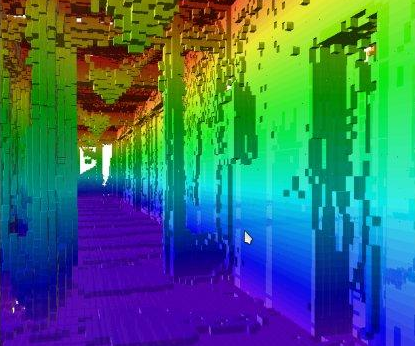
\includegraphics[width=\textwidth,height=4cm]{images/octomap.png}
	 	\caption{Mapa de ocupação (\textit{octomap})}
		\fonte{\\\cite{octomap}}
	 	\label{fig:octomap}
	\end{minipage}
	\begin{minipage}[b]{0.33\linewidth}
	    \centering
	    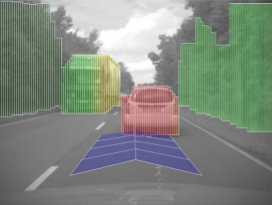
\includegraphics[width=\textwidth,height=4cm]{images/stixel.png}
	 	\caption{Segmentação por \textit{stixels}}
		\fonte{\cite{stixelworld}}
	 	\label{fig:stixel}
	\end{minipage}
\end{figure}

Devido à sua dimensionalidade, a informação a ser tratada é de ordem cúbica
comparada a ordem quadrática no caso planar. Algoritmos eficientes para tratar e
analisar tal volume de dados são necessários. O tratamento da informação deve
ser dado de forma volumétrica levando à necessidade de estruturas de dados
correspondentes. Largamente utilizado em computação gráfica, a representação por
\textit{voxels} é a abordagem tradicional pois permite discretizar o espaço em
sólidos cúbicos, reduzindo assim o espaço de busca. Uma técnica eficiente para a
representação de mapas tridimensionais é apresentada em \cite{octomap} e se
baseia no conceito de \textit{octrees}. Nesta abordagem o espaço é representado
por um \textit{octomap} (\fig{fig:octomap}), de acordo com a ocupação do espaço.
A informação da ocupação do espaço é obtida através de uma nuvem de pontos,
podendo esta ser fornecida de forma incremental, gerando então um mapa do espaço
de forma recursiva.

Outra abordagem de representação da informação tridimensional da cena em
agrupamentos por volumes é apresentada no trabalho de \cite{stixelworld}. Neste
trabalho é introduzido o conceito de \textit{stixel}, que representa um
determinado objeto a partir de sua projeção a partir do solo. O \textit{stixel}
é então um paralelepípedo (\fig{fig:stixel}) que representa uma região ocupada
na cena. Esta abordagem tem sido aplicada em reconhecimento de objetos na cena,
como veículos e pessoas \cite{Benenson2012}. O \textit{stixel} é dado por uma
base retangular e uma altura tendo o plano do chão como origem (representação
também chamada de 2,5 dimensões). Apesar de ser uma representação restritiva do
espaço tridimensional tem se demonstrado vantajosa principalmente em relação ao
seu custo computacional \cite{Benenson2011}.

%OSORIO
%> Ao final de cada capítulo sempre é bom ter uma seção de "Considerações
% Finais", na qual se faz uma reflexão do que foi apresentado (uma visão mais
% ampla de todo conteúdo) e aproveitando para fazer uma relação com o trabalho 
% como um todo e inclusive fazendo um "gancho" para o próximo capítulo

A construção e representação de mapas de ocupação por \textit{octree} se
apresenta mais vantajosa por ser uma representação estruturada dos dados,
enquanto os \textit{stixels} são independentes enquato estrutura de dados.
Porém, para classificação e clusterização de objetos na cena os \textit{stixels} já são
uma representação apropriada. Desta forma, utilizar ambas abordagens vem sendo
estudado com o propósito de agregar ambas características em um mapa de
navegabilidade.


%2012-10-15 Lido parcialmente (pode ser mais desenvolvido)
\section{Considerações Finais}
	
Neste capítulo foram apresentados os principais problemas referentes a navegação
autônoma do veículo relativos às questões de localização, mapeamento e
navegação. Em relação a localização, foi considerada uma proposta de utilização
de sensores do tipo GPS (para a localização) e de uma câmera estéreo (para o
mapeamento local e desvio de obstáculos). Por fim, foram apresentados e feita
uma breve análise sobre métodos de navegação. Baseado nas referências
analisadas, os métodos VFH e RNAs são soluções adequadas para uma navegação
baseada em uma orientação de destino, associada ao desvio de obstáculos
detectados através de uma percepção local. Estes elementos constituem-se
portando dos módulos e componentes deste projeto de pesquisa de mestrado. No
capítulo seguinte será apresentada a metodologia proposta.

%2012-10-14: Lido OK


\section{Mapeamento e Localização}
\label{sec:mapeamento_localizacao}

%A questão do mapeamento e localização é considerado um problema central na
%robótica móvel, 

O mapeamento e localização é uma necessidade recorrente nas aplicações em
robótica móvel, onde a caracterização do veículo como autônomo de fato pode vir
a ser dada essencialmente pela sua capacidade de tratar esta questão. Para que
um robô possa ir de um ponto ao outro do ambiente ele deve conhecer, pelo menos,
a sua localização e a localização do seu ponto de destino. Quando o mapa e a
estrutura do ambiente, assim como a localização do veículo, são desconhecidos a
priori essa questão se torna crítica. Esta necessidade é denominado de SLAM
(\textit{Simultaneous Localization and Mapping}) e é um problema central na
robótica móvel, onde ambas informações dependem uma da outra para serem obtidas. Um
algoritmo proposto para solucionar o SLAM é apresentado em \cite{Thrun2004} que
utiliza uma abordagem probabilística onde as estimativas tando da posição como
do mapeamento são atualizadas uma a partir da outra a medida que dados
sensoriais são coletados.

A visão computacional tem sido aplicada em soluções para o tratamento de SLAM
como a fonte de informação sensorial. Outros equipamentos, como sensor a laser
utilizado em \\\cite{Lategahn2011} e até mesmo sensores inerciais (IMU -
\textit{Inertial Measurement Unit}), como apresentado em \cite{FootSLAM}, são
aplicados e combinados com o propósito de aumentar a acurácia destas medições.
% a localização é estimada pelo onde o erro da estimativa da localização reduz a
% medida que o mapeamento Esse problema é normalmente tratado através de
% abordagens como o SLAM (\textit{Simultaneous Location and Mapping}).
% Uma solução robusta e eficiente para a questão de localização e mapeamento
% simultâneos (SLAM) na prática ainda é desafiadora (\cite{Dissanayake2001}) A
% visão computacional tem sido aplicada em soluções para o tratamento de SLAM ,
% onde uma abordagem recorrente no tratamento da localização e do mapeamento é a
% utilização de visão computacional.
% Porém há uma diversidade de sensores que podem ser integrados com o propósito
% de aumentar a acurácia destas medições, trabalhos recentes como o de
% \cite{FootSLAM} apresenta uma abordagem baseada em sensores inerciais (IMU -
% \textit{Inertial Measurement Unit}).
Entretanto, em ambientes externos (\textit{outdoor}) e extensos a construção de
um mapa global a partir dos dados sensoriais pode não ser viável, comprometendo
a estimação da localização baseada em mapa.
% e a definição da localização em relação a este mapa pode se tornar um problema
% intratável .
Uma solução para determinação da localização em ambientes externos é a obtenção
de coordenadas através do uso do GPS (\textit{Global Positioning System}), que é
baseado na trilateração das distâncias do veículo em relação a uma “constelação”
de satélites deste sistema. Portanto, a posição do veículo e de seu destino pode
ser estimada diretamente (com um certo erro) a partir das informações fornecidas
por um aparelho localizador GPS.



%OSORIO
%> Podia discutir um pouco mais sobre estas questões (expandir esta seção):
%- Dependência da existência de um mapa previamente definido (mapeado pelo robô
%ou não) e do planejamento prévio da rota do robô, ou, navegar no ambiente
%(usualmente não estruturado) sem o uso de um mapa ou de um planejamento prévio
%de rotas (existe o risco de ficar bloqueado, pois possui apenas o conhecimento
%local do ambiente e não realiza um plano global => é bom mostrar que está
%consciente disto).
%- Dependência de um mapa (global) exato e de uma localização exata, ou
%alternativamente, usa um mapa aproximado (local) e usa uma localização também
%aproximada (não muito precisa).
%> São abordagens possíveis e podemos "escolher" entre elas de acordo com o
%problema e requisitos impostos pela aplicação. Obviamente neste trabalho foi
%feita uma escolha (e espero que o leitor se convença que foi uma boa escolha
%dado o contexto)    :)


A localização pode se beneficiar quando há mapas previamente fornecidos, sendo
necessária a localização da posição inicial em relação ao mapa. Os mapas têm
papel importante na tarefa de navegação (seção \ref{sec:navegacao}), tanto
quando fornecidos previamente como quando construídos no momento em que o
veículo se desloca no ambiente. O mapa para navegação geralmente se caracteriza como
local ou global \cite{concepts}. O mapa global provê informações mais
abrangentes sobre o espaço onde o veículo irá se deslocar, principalmente
fornecendo informações sobre obstáculos estáticos e zonas navegáveis
preferenciais, como estradas. Estas informações dos mapas normalmente se
associam a custos, os quais são utilizados pelos algoritmos de planejamento
buscar o melhor caminho. Também, os mapas podem ser representados de forma
métrica (geométrica) e/ou topológica - contendo informações mais detalhadas de o
quê ocupa um determinado espaço (prédio, vegetação, etc.)\cite{Thrun98a}. Já os
mapas locais têm o papel de expressar o ambiente dentro do raio de atuação dos
sensores, ou seja, uma noção localizada próxima ao veículo. Estes mapa local
contém a visão mais atual do ambiente, contemplando obstáculos dinâmicos. A
construção do mapa local pode ser utilizado para agregar informações e atualizar
o mapa global, desta forma, o mapa global se traduz em uma memória do espaço
para o veículo (\fig{fig:map2d}). Quando não há informação prévia que possa ser
utilizada como mapa global é usual uma navegação prévia para o reconhecimento do
ambiente antes que se efetuem tarefas específicas de navegação. Este
reconhecimento inicial pode ser feito de forma autônoma apenas vagando no
ambiente como uma navegação guiada.

\begin{figure}[ht]
%	\centering
	\begin{minipage}[b]{0.9\linewidth}
	    \centering
	    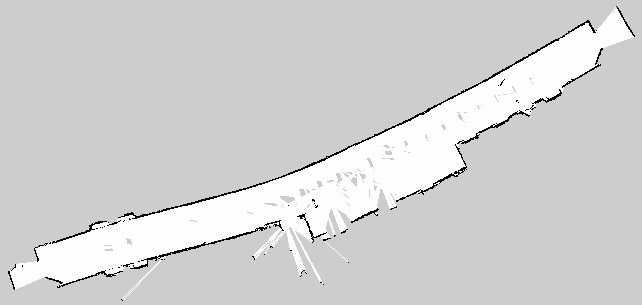
\includegraphics[width=\textwidth,height=6cm]{images/map_2d.jpg}
	 	\caption{Mapa de ocupação planar: Em branco o espaço live, em preto o espaço
	 	ocupado e em cinza o espaço sem informação de ocupação}
		\fonte{www.ros.org (divulgação)}
	 	\label{fig:map2d}
	\end{minipage}
\end{figure}

%2012-10-15 Lido OK (pode ainda ser mais desenvolvido)


\section{Informação Sensorial: Visão Computacional}

Um veículo móvel terrestre se desloca (geometricamente) apoiado sobre um plano
de suporte, ou seja, seus graus de liberdade usualmente podem ser considerados
em duas dimensões. Desta forma, o reconhecimento do chão representa uma
necessidade e se caracteriza um importante desafio ao se considerar um ambiente
externo não estruturado composto por um solo com vegetação. Além da detecção do
chão, é necessária uma certa classificação das regiões deste plano de suporte
(solo) como sendo, por exemplo, uma superfície transitável ou não transitável:
devido à presença de vegetação, obstáculos, buracos e demais impedimentos.
Os sensores típicos, como sonares e lasers, não apresentam dados muito adequados
para viabilizar essa classificação, uma vez que o sonar possui uma limitação de
alcance e de precisão e o sensor laser de 1 feixe é capaz apenas de analisar uma
seção planar do espaço tridimensional (além de ter um custo muito elevado para
certas aplicações). As câmeras de vídeo são mais adequadas para capturar tais
informações que caracterizam o ambiente, principalmente, se forem usadas câmeras
estéreo, das quais é possível extrair uma informação de profundidade dos
elementos da cena capturada. A utilização de câmeras de vídeo demandam algumas
tarefas elementares, como o ajuste de foco, a utilização de lentes adequadas ao
ângulo de visão necessário e uma devida calibragem. A calibragem das câmeras é
um processo fundamental para se obter um sistema de visão computacional com
representação tridimensional a partir de um par de câmeras independentes
(binocular). Neste processo são calculados (estimados) os parâmetros internos e
externos de cada câmera. Estes parâmetros são essenciais para a reconstrução
tridimensional a partir das imagens capturadas pela câmera estéreo
\cite{Faugeras1993}.

A estimação dos parâmetros internos (intrínsecos) consiste em se obter a
distância focal e o ponto central da imagem, que por questões de alinhamento
entre lentes e sensor pode não ser o pixel central da imagem, influenciando
fortemente os demais processos de estimação \cite{WilsonShafer1994}. Estes
dois parâmetros definem como a imagem é formada por uma câmera estilo
estenopeica (\textit{pin-hole}) e a sua projeção perspectiva. Outros parâmetros
também internos, não associados com o modelo de projeção e sim com as
características físicas das lentes utilizadas, também são estimados no processo
de calibragem. No caso das câmeras de vídeo existe a necessidade de utilização
de lentes, tanto para reduzir a imagem a ser projetada no sensor (filme/CCD)
como para aproximá-las. As lentes comumente são estruturas com curvatura
esférica, característica esta que provoca distorções óticas na imagem projetada.
Estes efeitos são chamados de distorções radiais, produzindo imagens com
demonstrado na \fig{fig:distortions}, nos casos, onde esta distorção pode ser em
forma de “barril” (\textit{barrel}) ou “almofada” (\textit{pincushion})
\cite{Weng1992}.

% (\fig{fig:int_param}).
As distorções óticas influenciam fortemente de forma negativa o processo de
correspondência entre as imagens para extrair a informação tridimensional, sendo
grande fonte de ruído quando não corrigidas. É interessante notar que,
matematicamente, o processo de correção das distorções óticas se baseia na
curvatura esférica da lente, porém as lentes são formadas por uma composição de
várias camadas com curvaturas diferentes (\fig{fig:lens}), que ainda podem
apresentar defeitos no processo de fabricação. Portanto, o modelo matemático
utilizado na correção é sempre uma aproximação global do aparato ótico, fonte
por si só de imprecisão \cite{WilsonShafer1994}.

%Existem ainda outros
%parâmetros que podem ser considerados, porém, estes estão associados a questões
%técnicas da forma de aquisição da imagem e não à formação da imagem propriamente
%dita, portanto são subjetivas ao aparato utilizado sendo necessárias ou não, a
%exemplo, os problemas referentes ao entrelaçamento e varredura da imagem.

% \begin{figure}[ht]
% 	\centering
% 	\begin{minipage}[b]{0.3\linewidth}
% 	    \centering
% 	    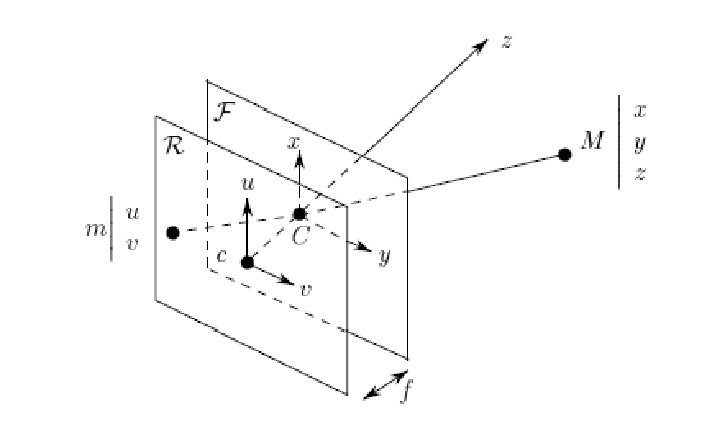
\includegraphics[width=\textwidth]{images/int_param.png}
% 	 	\caption{Ponto central e distância focal}
% 		\fonte{(\cite{Faugeras1993})}
% 	 	\label{fig:int_param}
% 	\end{minipage}
% 	\hspace{0.1cm}
% 	\begin{minipage}[b]{0.3\linewidth}
% 	    \centering
% 	    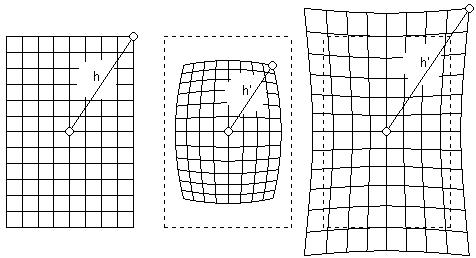
\includegraphics[width=\textwidth]{images/distortions.png}
% 	 	\caption{Distorções óticas}
% 	 	\label{fig:distortions}
% 	\end{minipage}
% 	\hspace{0.1cm}
% 	\begin{minipage}[b]{0.3\linewidth}
% 		\centering
% 	    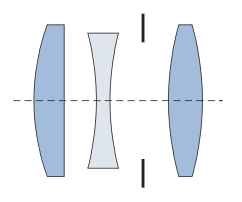
\includegraphics[width=\textwidth,height=3cm]{images/lens.png}
% 	 	\caption{Exemplo de composição ótica}
% 	 	\label{fig:lens}
% 	\end{minipage}
% \end{figure}

\begin{figure}[ht]
	\centering
	\hspace{0.1cm}
	\begin{minipage}[b]{0.45\linewidth}
	    \centering
	    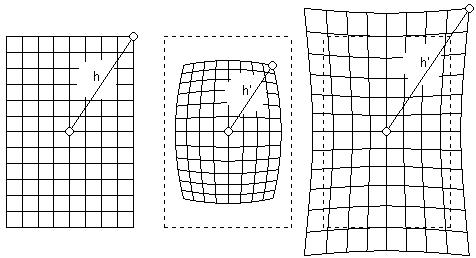
\includegraphics[width=\textwidth]{images/distortions.png}
	 	\caption{Distorções óticas: sem distorção (\textit{esquerda}), 
	 	distorção tipo “barril” (\textif{centro}), 
	 	distorção tipo “almofada” (\textit{direita}).}
	 	\label{fig:distortions}
	\end{minipage}
	\hspace{0.1cm}
	\begin{minipage}[b]{0.45\linewidth}
		\centering
	    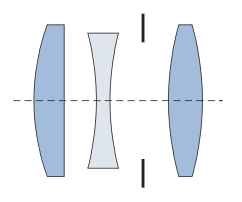
\includegraphics[width=\textwidth,height=4cm]{images/lens.png}
	 	\caption{Exemplo de composição ótica de lentes.}
	 	\label{fig:lens}
	\end{minipage}
\end{figure}


De posse dos parâmetros internos associados às distorções é necessário um
pré-processamento para a sua correção que ao ser aplicado produz uma imagem mais
própria para os algoritmos de correspondência que formarão a imagem
tridimensional. Os parâmetros internos são também chamados de parâmetros do
modelo, isto é, como a imagem é formada. Um outro modelo de câmera geralmente
associado a veículos móveis são as câmeras omnidirecionais, capazes de produzir
uma imagem em 360 graus, útil para veículos com esse grau de liberdade de
movimentos. A calibragem deste tipo de câmera é ainda mais complexa. O segundo
conjunto de parâmetros são os parâmetros externos (extrínsecos), também chamados
de parâmetros de pose. Este conjunto diz respeito à posição da câmera em relação
ao ambiente, no caso, a um sistema de coordenadas referencial. Estes são os
principais parâmetros para a reconstrução tridimensional, pois são utilizados
para se chegar a uma correspondência entre os pixeis de cada uma das duas
imagens. Esta correspondência entre os pontos é obtida pelos princípios da
geometria epipolar (\fig{fig:epipolar}) \cite{Faugeras1993}. De posse dessa
correspondência, a partir do deslocamento destes pontos (disparidade) e um
processo de triangulação, pode ser construída uma representação tridimensional
em um mapa de profundidade. Fundamentalmente, são determinados os planos
formados pelos pontos em comum em cada imagem (referenciais obtidos pela
calibragem) e o ponto central de cada imagem. Esses planos no espaço (ambiente)
são coincidentes, ou seja, o mesmo plano de corte. Esta projeção do plano em
cada imagem definem retas, chamadas retas epipolares. Desta forma é possível
fazer a correspondência dos demais pontos (não referenciais). Este alinhamento
das imagens é chamado de retificação \cite{Fusiello2000}, como pode ser visto
na \fig{fig:rectification}. Pela geometria epipolar todos os planos formados
pelos pontos referenciais serão concorrentes e as suas intersecções se dão em
uma reta em comum, chamada linha base. Esta linha base determina o alcance da
visão (profundidade).

Em um estudo anterior realizado por Klaser \cite{Klaser2007}, em seu trabalho
de conclusão de graduação (TCC), foi aplicada visão tridimensional para
monitorar experimentos de laboratório utilizando como processo de calibragem o
método de Tsai \cite{Tsai1987}. Naquele trabalho, onde as duas câmeras podiam
ser posicionadas em relação ao ambiente com uma certa liberdade observando-se
alguns critérios, foi possível verificar que um conjunto de referenciais capazes
de descrever os três planos ortogonais do espaço tridimensional produziam uma
calibragem bastante precisa. Para isso, foi utilizado um molde semelhante ao
canto de uma sala contendo pelo menos três pontos referenciais em cada parede e
no chão (\fig{fig:bioview}). Uma vantagem do método de Tsai é que o referencial
para a calibragem é dado informando sua posição na imagem e sua posição real no
ambiente, sendo a posição real dada de forma relativa a um sistema de
coordenadas referencial no espaço. Com isso, ao extrair a informação
tridimensional de um ponto pelo processo de triangulação a partir da calibragem
do par estéreo, a informação resultante contém as coordenadas espaciais do ponto
na unidade de medida adotada. Desta forma, é possível saber a posição real de um
determinado ponto, podendo ser extraída uma nuvem de pontos 3D do ambiente
(\textit{3D point cloud}). Porém, para se obter as coordenadas tridimensionais
de um determinado ponto no espaço é necessário saber onde esse ponto se encontra
em cada imagem \cite{MundyZisserman1994}.
Isto não é trivial, mas é possível utilizar métodos de detecção e casamento
(\textit{matching}) de características (\textit{features}) das imagens para
buscar a correspondência, como por exemplo, o método SIFT
(\textit{Scale-Invariant Feature Transform}) \cite{Lowe1999} e o método SURF
(\textit{Speeded Up Robust Features}) \cite{Bay2008}.
% Uma abordagem baseada neste princípio em que, a partir de duas poses da mesma
% cena, se extrai uma terceira coordenada tendo por base uma calibragem das
% câmeras e um processo de correlação global dos pixeis, é chamada de mapa de
% disparidade. Este processo é computacionalmente custoso e existem diversas
% técnicas para a sua implementação.
Uma abordagem para extrair a terceira coordenada espacial tendo por base duas
imagens da mesma cena em poses diferentes e a devida calibragem é chamada de
disparidade \cite{Qian97binoculardisparity}. Este processo é computacionalmente
custoso e existem diversas técnicas para a sua implementação.

\begin{figure}[ht]
	\begin{minipage}[b]{0.3\linewidth}
	    \centering
	    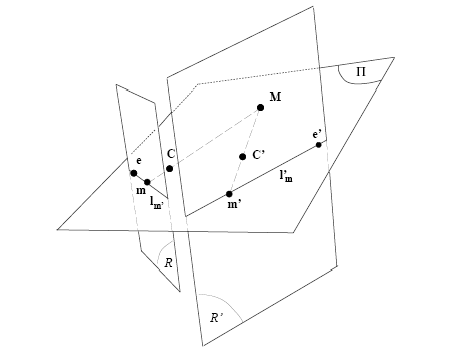
\includegraphics[width=\textwidth]{images/epipolar.png}
	 	\caption{Geometria epipolar}
		\fonte{\cite{Faugeras1993}}
	 	\label{fig:epipolar}
	\end{minipage}
	\hspace{0.1cm}
	\begin{minipage}[b]{0.3\linewidth}
	    \centering
	    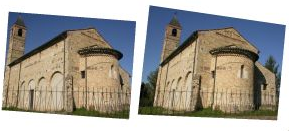
\includegraphics[width=\textwidth,height=4cm]{images/rectification.png}
	 	\caption{Retificação }
		\fonte{Andrea Fusiello}
	 	\label{fig:rectification}
	\end{minipage}
	\hspace{0.1cm}
	\begin{minipage}[b]{0.3\linewidth}
		\centering
	    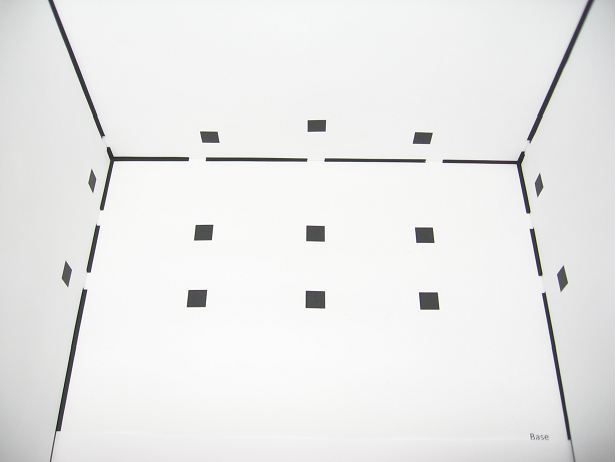
\includegraphics[width=\textwidth,height=4cm]{images/bioview.png}
	 	\caption{Calibragem com referenciais fixos}
		\fonte{\cite{Klaser2007}}
	 	\label{fig:bioview}
	\end{minipage}
\end{figure}

\vspace{0.5cm}


%OSORIO
%> Podia acrescentar uma breve seção sobre GPS:
%2.3 Sensores: Localização e Orientação
%descrevendo sobre a posição (GPS) e orientação (bússola), do veículo e de seu
% destino.
%> O parágrafo abaixo já é uma espécie de "resumo e consolidação" do que foi
%apresentado nas seções anteriores.

Portanto, neste trabalho serão adotados os sensores do tipo GPS e Bússola
(posição e orientação) para localização e câmeras estéreo para a extração de
mapas locais. Estes mapas descreverão o ambiente e os obstáculos através de uma
representação espacial (3D) na qual se encontra o veículo robótico autônomo. A
câmera estéreo irá fornecer um mapa de navegabilidade local composto por
informações obtidas a partir do mapa de disparidade que será descrito a seguir.

%OSORIO
%> Senti falta de uma noção mais geral sobre como passamos da parte de visão
% computacional estéreo para os mapas locais (mapa 3D - cloud of points, mapa local, mapa de navegabilidade). 
% Mapa de disparidade já entra em um conceito específico...
%> Talvez pudesse ter citado o trabalho do Caio (mestrado) e do Patrick
% (mestrado) que tem bons exemplos de mapas (com figuras)  :)


% 2012-10-13 lido OK


\section{Mapas de Disparidade}
\label{sec:mapas_disparidade}

Os mapas de disparidade se tornaram uma ferramenta bastante utilizada para a
percepção tridimensional. Para robôs móveis autônomos os mapas de disparidade
são muito úteis, principalmente na detecção e desvio de obstáculos. O veículo
pode extrair uma informação de profundidade que servirá como parâmetro para a
navegação, por exemplo, uma região frontal de maior profundidade pode
representar um caminho sem obstáculos, livre de objetos e elementos localizados
em frente a câmera. Atualmente, a implementação direta em hardware dos
algoritmos de cálculo do mapa de disparidade a partir de um par de imagens
(câmera estéreo) permite a aplicação em tempo real e de forma embarcada
(\fig{fig:stoc_on_chip}) \cite{Khaleghi2008}.

A ideia fundamental do mapa de disparidade é fornecer uma informação de
profundidade relativa, mapeada diretamente na imagem bidimensional a partir do
valor do pixel. Usualmente são utilizadas imagens em tons de cinza (8
\textit{bits}), fornecendo então até 255 níveis de profundidade. Na
\fig{fig:tsukuba}, o mapa de disparidade está representando os obstáculos mais
próximos por tons mais claros e os obstáculos mais distantes por tons mais
escuros. Desta forma, os pixeis da imagem passam a representar no lugar da
informação de cor ou luminosidade uma informação de profundidade sobre os
elementos da cena. Os dispositivos sensores que fornecem uma imagem colorida
juntamente com o mapa de disparidade têm sido denominados de dispositivos RGB-D
(Imagem RGB + \textit{Depth}/mapa de disparidade). O sensor Kinect da
Microsoft\foot{Microsoft Kinect - http://www.xbox.com/en-us/kinect} fornece
imagens RGB-D com uma precisão de 2047 níveis de profundidade. Uma avaliação da
qualidade do mapa de disparidade produzido pelo Kinect \cite{Khoshelham2012}
mostrou que a relação entre o nível de profundidade e distância não é linear,
onde a distância real dos objetos é gradualmente maior do que a distância
estimada a medida que se afastam da câmera. O Kinect é utilizado atualmente como
base de comparação pois é uma aplicação em larga escala comercial desta técnica
e produz resultados práticos satisfatórios.

\vspace{0.5cm}
\begin{figure}[h!!!]
	\centering
	\begin{minipage}[b]{0.4\linewidth}
	    \centering
	    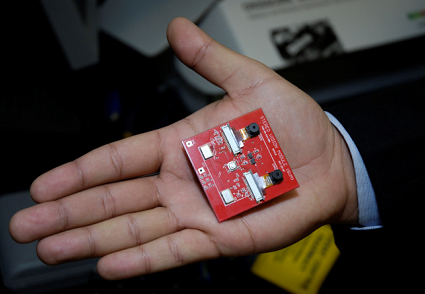
\includegraphics[width=\textwidth,height=4.5cm]{images/stoc_on_chip.png}
	 	\caption{Sistema de visão tridimensional
embarcado baseado em mapa de disparidade}
		\fonte{\cite{Khaleghi2008}}
	 	\label{fig:stoc_on_chip}
	\end{minipage}
	\hspace{0.1cm}
	\begin{minipage}[b]{0.55\linewidth}
	    \centering
	 	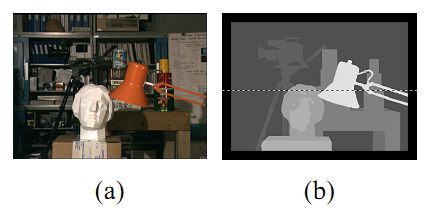
\includegraphics[width=\textwidth,height=4.5cm]{images/tsukuba.png}
	 	\caption{Estéreo: \textbf{(a)} imagem RGB \\ \textbf{(b)} disparidade referencial}
		\fonte{University of Tsukuba}
	 	\label{fig:tsukuba}
	\end{minipage}
\end{figure}

%Porém, essa não linearidade não é um artefato
%que resulta propriamente daquela implementação, 
%ela advém do fato de o mapa ser
%gerado a partir de imagens que são formadas pela projeção perspectiva que 
%inerentemente produz esse efeito (\textit{foreshortening}).

Em sistemas onde as câmeras são estacionárias (fixas em um local), como na
aplicação tradicional do Kinect, técnicas de extração e supressão do fundo podem
ser utilizadas para aumentar a robustez do método \cite{Ivanov2000}. No caso das
aplicações em robótica móvel, as câmeras estão em constante movimento
potencializando estes efeitos negativos, fazendo-se necessário outros métodos
para minimizar estes efeitos. Outra característica a ser apontada em relação ao
Kinect é sua inviabilidade de uso no ambiente externo, ou seja, com iluminação
natural - isto se deve ao fato da tecnologia empregada se basear em luz
estruturada e requer iluminação artificial (infra-vermelho) a qual sofre
interferência na presença de luz solar. Em ambiente externo são utilizadas
câmeras convencionais, onde o conjunto estéreo pode ser constituído tanto por
câmeras independentes permitindo maior versatilidade de poses como no uso de
câmeras do tipo STOC (\textit{STereo On a Chip}) que são mais estáveis em
relação à manutenção da calibragem.

%Em ambiente externo são utilizadas câmeras convencionais
%porém geralmente o uso de câmeras estéreo tipo STOC (\textit{STereo On a Chip})
%são um tipo de aplicação por serem mais estáveis em relação à manutenção da
%calibragem devido a vibrações.

%Fig. 2.7: Sistema de visão tridimensional
%embarcado baseado em mapa de disparidade
%Fonte: 
%Fig. 2.8: a) Imagem RGB; b) Mapa de disparidade Fonte: University of Tsukuba 

O mapa de disparidade provê uma percepção espacial que representa os elementos
da cena em um espaço tridimensional, fornecendo assim, uma fonte muito rica de
informações sobre a cena. A partir destas informações pode ser possível então
definir a trajetória do veículo de modo a desviar dos obstáculos que se
encontram a sua frente ao mesmo tempo em que este se locomove em direção ao seu
destino. Este processo é denominado de navegação robótica e será detalhado a
seguir.


%%2012-10-14 Lido OK

\section{Navegação}
\label{sec:navegacao}

A navegação em campo aberto se torna um problema de tomada de decisões difícil,
devido à ausência de um mapa global atualizado, a falta de referenciais locais e
o excesso de ruído dos sensores, que produzem pouca informação válida para o
sistema. Apesar do veículo estar buscando um destino preestabelecido, dirigir-se
sempre em linha reta pode não ser a melhor decisão, ou mesmo impossível. Além
disto, a indicação da posição atual (localização) pode não ser totalmente
confiável.

Ainda que se utilize GPS, esse sistema apresenta erro na localização exata
(usualmente com um erro médio de cerca de 5
metros\foot{http://en.wikipedia.org/wiki/Error\_analysis\_for\_the\_Global\_Positioning\_System}),
pois considera-se também o fato de que o veículo não tem uma estrada ou via como
referência (ambiente não estruturado). Já no caso de dispositivos como o
odômetro, utilizados para manter um controle da localização por
\textit{dead-reckoning} \cite{Dudekbook}, a confiabilidade é ainda menor pois
há grande tendência de discrepância uma vez que o erro é cumulativo. Estas
discrepâncias podem ser resultantes de derrapagens das rodas, erros de estimação
da real distância percorrida ou mesmo das alterações involuntárias de direção do
veículo. Uma possível melhoria da precisão do GPS pode ser conseguida usando um
sistema de correção DGPS (GPS diferencial), onde antenas em solo são utilizadas
para aumentar a precisão do local estimado pelos sinais dos satélites. No
entanto, nem sempre este tipo de abordagem é possível pela falta desta
infraestrutura no local desejado, além de possuir um custo bem mais elevado em
relação a abordagem tradicional. No Brasil, o IBGE\foot{IBGE –
http://www.ibge.gov.br} disponibiliza serviços de posicionamento de precisão
através da RBMC\foot{RBMC –
http://www.ibge.gov.br/home/geociencias/geodesia/rbmc/rbmc.shtm} (Rede
Brasileira de Monitoramento Contínuo). O GPS tradicional possui um erro médio
usual entre 5 a 10 metros da posição estimada informada em relação a posição
real, enquanto um DGPS pode reduzir este erro médio para menos de 1 metro
(aproximadamente 50 cm).

É interessante observar que em aplicações de GPS em roteiros rodoviários (e
urbanos) a existência de um mapa local permite um certo ajuste de coerência que
visualmente dá a impressão de uma maior precisão, porém em campo aberto esta
abordagem não é possível. Existe inclusive um “jogo”, denominado de
GeoCaching\foot{GeoCaching Game:
http://www.geocaching.com/guide/default.aspx}, inspirado nesta ideia de
navegação baseada em GPS, onde o usuário deve encontrar um ponto de destino
usando como informação apenas as coordenadas GPS disponíveis, logo, a
dificuldade é exatamente a imprecisão. 

O algoritmo básico de navegação de um veículo autônomo pode se basear em um
princípio estratégico similar ao utilizado por uma pessoa portadora de
deficiência visual, ou seja, passos controlados e o constante monitoramento do
ambiente ao seu redor. Uma pessoa consegue achar, de modo intuitivo e racional,
um caminho em direção a um determinado destino e evitar colisões com obstáculos
em seu caminho. No caso de um veículo autônomo, este não possui essa capacidade
intrínseca de navegação e desvio de obstáculos, devendo ser dotado de algum
recurso computacional e/ou físico para tal. Existem diversos algoritmos
clássicos de estratégia de navegação, como por exemplo, o algoritmo do
\textit{bug} \cite{Choset2005} e suas variantes \cite{Taylor2009}, que se
baseiam na detecção de bordas (obstáculos) e executam a locomoção aproximando-se
a elas e fazendo o seu contorno.


\subsection{Planejamento}

A operação de navegação requer um planejamento, este planejamento pode ser
categorizado como local ou global. No planejamento global há a necessidade de
que o ambiente seja previamente conhecido através da representação de um mapa
global (geralmente estático), enquanto que o planejamento local se baseia apenas
na posição onde o robô se encontra e no alcance dos seus sensores. As
metodologias de planejamento podem ser agrupadas em quatro categorias
principais: gráficas, clássicas, heurísticas e de campo potencial. As
metodologias baseadas em campos potenciais são soluções elegantes que se baseiam
em forças de repulsão aos obstáculos e forças de atração ao destino, podendo ser
aplicado para o planejamento local. Porém, de acordo com o tipo de ambiente em
que o robô se encontra podem apresentar problemas relacionados a mínimos locais
devido a forças de repulsão demasiadas que inibem o movimento do robô. Em
ambientes abertos e com poucos obstáculos os campos potenciais são uma abordagem
largamente adotada. O VFH (\textit{Vector Field Histogram})
\cite{Borenstein1991} aplica esta ideia e teve como proposta inicial a tentativa
de evitar os mínimos locais, dentro do que for possível com relação as
informações sensoriais disponíveis.

%proposta inicial a solução
%da questão dos mínimos locais.

%Uma técnica em destaque na abordagem de campos potenciais é
%o VFH (\textit{Vector Field Histogram}) (\cite{Borenstein1991}), que soluciona
%diversos problemas associados a este tipo de abordagem.

O método VFH foi projetado para ser utilizado em tempo real a partir dos dados
dos sensores, gerando um histograma (\fig{fig:vfh}) onde os picos representam a
proximidade dos objetos em relação ao veículo e os vales os espaços livres.
Idealizado para ser utilizado com sensores do tipo sonar, leva em conta as
questões inerentes a ruídos próprios desta classe de sensor e as características
cinemáticas do veículo.

%, sendo base para
%outros métodos que utilizam esta abordagem de campo potencial/campo de força.

\vspace{0.5cm}
\begin{figure}[ht]
	\centering
	\begin{minipage}[b]{1\linewidth}
	    \centering
	    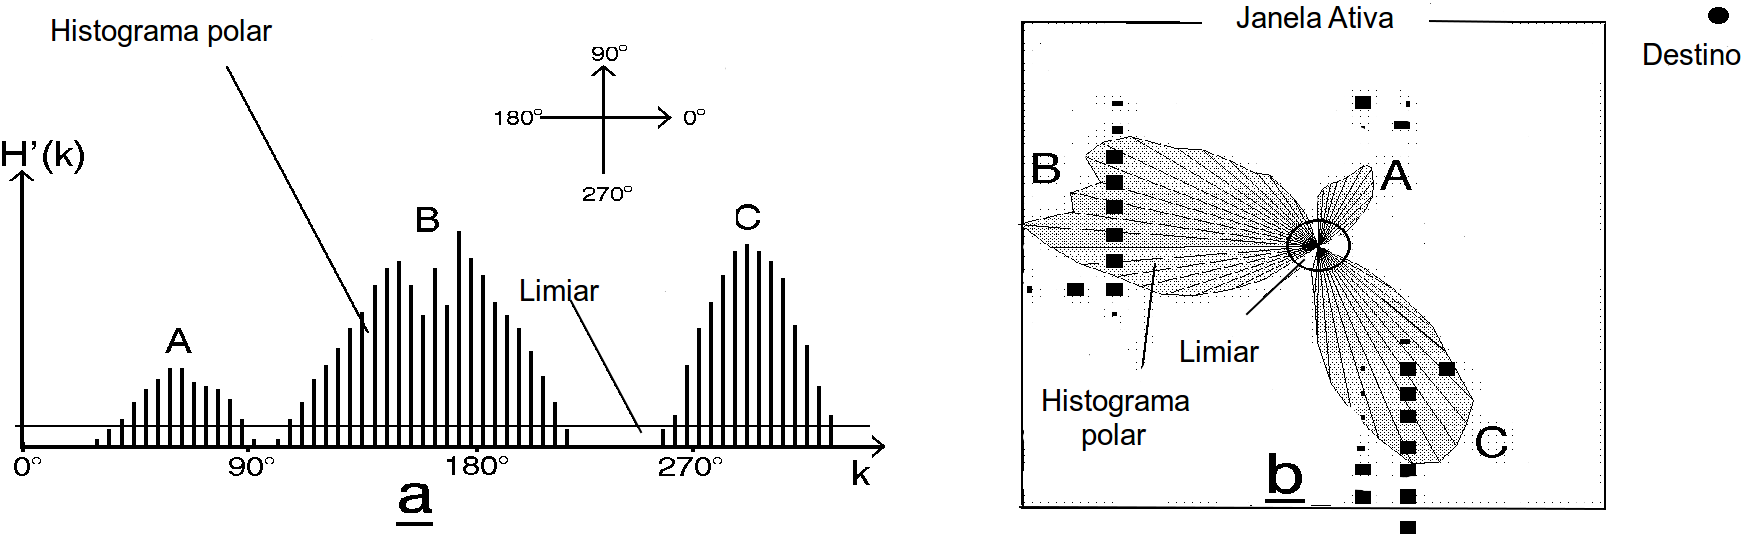
\includegraphics[width=\textwidth,height=7cm]{images/vfh_horiz.png}
	 	\caption{VFH - \textbf{(\underline{a})} Gráfico do histograma, 
	 	onde H'(k) representam as forças de repulsão aos obstáculos nas direções k.\\
	 	\textbf{(\underline{b})} Representação espacial em relação aos 
	 	obstáculos (retângulos em preto) - A área circulada representa a posição do robô.}
		\fonte{adaptado de: \cite{Borenstein1991}}
	 	\label{fig:vfh}
	\end{minipage}
\end{figure}


%Para o planejamento global, de posse de uma mapa convertido em custos 

Enquanto o VFH tem um comportamento mais reativo, em um cenário onde um mapa
global mesmo que incompleto é fornecido pode ser adotado um método deliberativo
para o planejamento da trajetória até um destino.

Os algoritmos de geração de trajetória baseados em amostras tem sido adotado em
robótica móvel com maior ênfase principalmente pela aplicabilidade prática, este
tipo de abordagem leva em consideração a cinemática do veículo gerando
trajetórias realistas com custo computacional baixo \cite{ompl}.

Estes métodos inicialmente constroem um grafo baseado em amostras de trajetórias
que o veículo pode executar, onde geralmente se limita a algumas manobras afim
de reduzir as ramificações do grafo \cite{topologic}. Após esta etapa pode ser
executado um método gráfico de busca por um caminho de menor custo baseado no
menor caminho e proximidade de obstáculos \fig{fig:sbpl}.

\begin{figure}[ht]
	%\hspace{0.1cm}
	\centering
	\begin{minipage}[b]{1\linewidth}
	    \centering
	 	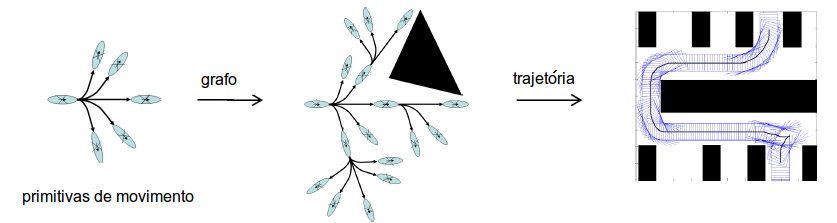
\includegraphics[width=\textwidth,height=5cm]{images/sbpl.png}
	 	\caption{Planejamento de trajetória por amostras}
	 	\fonte{adaptado de: www.ros.org}
	 	\label{fig:sbpl}
	\end{minipage}
\end{figure}
%No trabalho de \cite{} foi utlilizada a biblioteca SBPL
%(\textit{Search-based Planning Library}) 

%Os métodos heurísticos
% baseados em amostra 

\subsection{Controle}

O controle de navegação de um robô móvel pode ser classificado basicamente como
reativo, deliberativo ou híbrido \cite{Wolf2009}, podendo ser estruturada de
forma hierárquica; um caso particular de arquitetura híbrida em camadas. No
projeto COHBRA \cite{Heinen2002}, foi utilizada a abordagem híbrida em camadas
para a criação de um sistema de controle para robôs móveis. Esta abordagem
híbrida permite ao sistema de controle planejar e executar um plano de uma
trajetória (camada deliberativa) ao mesmo tempo em que detecta a presença e
desvia de obstáculos que não foram previamente mapeados (camada reativa). As
técnicas aplicada na elaboração do sistema de controle podem ser baseadas em
Máquinas de Estados Finitos (FSM – \textit{Finite State Machines}), Sistemas
Especialistas e/ou Sistemas Nebulosos (FIS - \textit{Fuzzy Inference Systems}),
Redes Neurais Artificiais (RNA), ou mesmo, uma combinação destes em diversas
camadas. 

As RNAs são consideradas sistemas "caixa-preta": após o treinamento da RNA os
pesos sinápticos associados a cada neurônio (por exemplo, perceptron) não têm
propriamente um “significado”, somente valores numéricos que representam o
conhecimento adquirido. A sua capacidade de generalização torna-a tolerante a
ruídos e permite a aplicação principalmente quando não se consegue estruturar
totalmente o problema a partir de regras bem definidas. É uma técnica
extremamente plástica, podendo ser aplicada a diversas classes de problemas. O
sistema SEVA3D \cite{Heinen2007} se baseou no aprendizado neural de um FSM
(Finite-State Machine) para fazer o controle de navegação do veículo, já no
simulador RoBombeiros \cite{Pessin2008}, adotou-se uma RNA para este fim
(\fig{fig:ann_pesin}).

\vspace{0.5cm}
\begin{figure}[ht]
	%\hspace{0.1cm}
	\centering
	\begin{minipage}[b]{0.6\linewidth}
	    \centering
	 	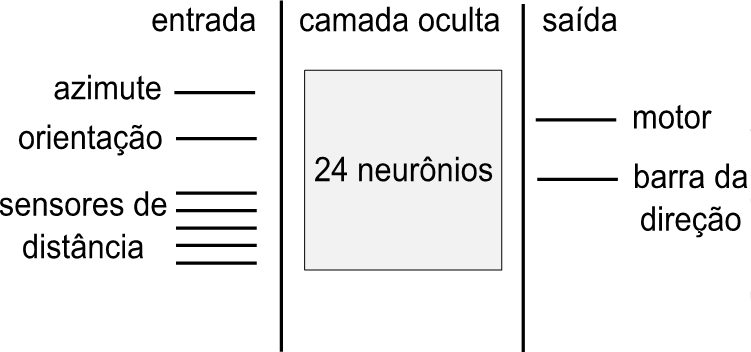
\includegraphics[width=\textwidth,height=5cm]{images/ann_pesin.png}
	 	\caption{Arquitetura da RNA no simulador RoBombeiros}
	 	\label{fig:ann_pesin}
	\end{minipage}
\end{figure}


%OSORIO
%> Podia detalhar um pouco mais sobre o Robombeiros aqui... se não for detalhar
% mais adiante, seria bom ser mais "didático" pois nem todos da banca sabem do
% que se trata e como funciona (assim como os futuros leitores deste texto)

No caso dos RoBombeiros, o controle pela rede neural era de um comportamento
basicamente reativo, onde ao mesmo tempo que direcionava o veículo para o
destino gerava comandos de desvio na presença de obstáculos próximos. Nesta rede
neural foi projetado como entrada a orientação do veículo dada por uma bússola e
a sua orientação em relação ao ponto de destino calculada pelas posições de GPS,
assim como informações sensoriais de distâncias de objetos presentes no raio de
ação do sensor laser utilizado. Desta forma a rede neural foi treinada para
gerar comandos de aceleração e esterçamento que controlavam a navegação do
veículo autônomo.

%2012-10-15 Lido OK

\section{Considerações Finais}
	
Neste capítulo foram apresentados os principais problemas referentes a navegação
autônoma do veículo relativos às questões de localização, mapeamento e
navegação. Em relação a localização, foi considerada uma proposta de utilização
de sensores do tipo GPS (para a localização) e de uma câmera estéreo (para o
mapeamento local e desvio de obstáculos). Por fim, foram apresentados e feita
uma breve análise sobre métodos de navegação. Baseado nas referências
analisadas, os métodos VFH e RNAs são soluções adequadas para uma navegação
baseada em uma orientação de destino, associada ao desvio de obstáculos
detectados através de uma percepção local. Estes elementos constituem-se
portando dos módulos e componentes deste projeto de pesquisa de mestrado. No
capítulo seguinte será apresentada a metodologia proposta.

%2012-10-14: Lido OK

\chapter{Metodologia} 
\label{cap:metodologia}

%O objetivo deste trabalho é desenvolver um sistema de navegação autônoma baseado em
%visão computacional a fim de capacitar um veículo terrestre a se locomover em ambientes externos
%não estruturados, ou seja, um campo com vegetação/plantação e/ou floresta pouco densa. O veículo
%deverá ser capaz de desviar de obstáculos de forma autônoma, e se dirigir até uma
%localização determinada escolhendo por meios próprios o caminho a seguir. Deverá ter alguma
%capacidade de reconhecer o terreno que irá se deslocar a fim de evitar zonas não transponíveis ou
%muito acidentadas.

No capítulo anterior foram apresentados os principais problemas referentes a
navegação autônoma do veículo relativos às questões de localização, mapeamento e
navegação. Em relação a localização, está sendo considerada uma proposta de
utilização de sensores do tipo GPS e bússola e de uma câmera estéreo para o
mapeamento e desvio de obstáculos. Baseado nas referências analisadas, os
métodos VFH e RNAs são soluções adequadas para uma navegação baseada em uma
orientação de destino, associada ao desvio de obstáculos detectados através de
uma percepção local. Em \cite{caio} foi utilizado o VFH para desvio de
obstáculos utilizando como informação sensorial dados de uma câmera estéreo. O
histograma polar utilizado pelo método VFH foi gerado a partir da informação de
profundidade obtida pela câmera estéreo. 


%Estes elementos constituem-se portando
%dos módulos e componentes deste projeto, onde as ferramentas usadas e a
%arquitetura geral do sistema serão detalhadas a seguir.

%de pesquisa de mestrado. No capítulo seguinte será apresentada a metodologia proposta.


No sistema RoBombeiros \cite{Pessin2008} foi implementada uma solução baseada em
coordenadas GPS para localização e uma RNA para o controle e navegação. O
sistema foi projetado para ambientes externos onde os veículos tinham como meta
o combate à incêndios florestais. Este sistema foi testado apenas em simulação
que consistia em ambientes não estruturados onde a vegetação predominante
era composta por árvores. Os veículos foram capazes de desviar dos obstáculos
adequadamente e se dirigir ao destino estabelecido (\fig{fig:incendio}). 


\begin{figure}[ht]
	\begin{minipage}[b]{0.95\linewidth}
	    \centering
	    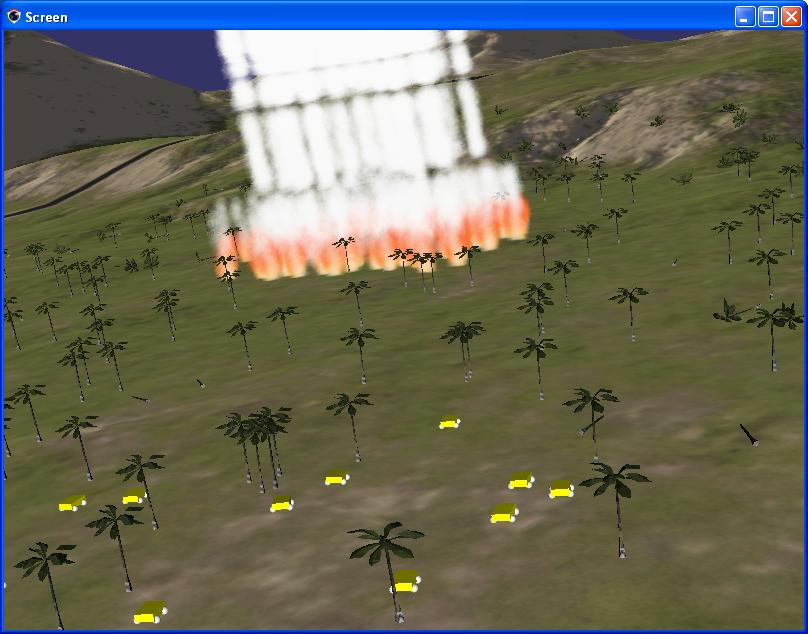
\includegraphics[width=12cm]{images/fogo30905osg.jpg}
	 	\caption{RoBombeiros - Navegação em ambiente não estruturado e estratégia de
	 	combate a incêndio florestal.}
	 	\label{fig:incendio}
	\end{minipage}
\end{figure}

Apesar do trabalho de \cite{Pessin2008} ter dado grande foco no combate à
incêndios e nas estratégias de deslocamento e atuação de um grupo de veículos,
este projeto irá se focar em um único veículo. Para os testes práticos será
avaliada apenas a capacidade de chegada ao destino com sucesso, dado que para
os experimentos em ambiente real somente a navegação estará sendo validada.


%Estes elementos constituem-se portando dos módulos e componentes deste projeto,
%onde as ferramentas usadas e a arquitetura geral do sistema serão detalhadas a
%seguir.

%\section{Objetivos Específicos}

Os principais objetivos específicos deste projeto de mestrado, que se apresentam
como um desdobramento do objetivo geral descrito acima, são:

\begin{itemize}

\item Extração de referenciais a partir de um par de câmeras, constituindo um
sistema de visão binocular (estéreo);

\item Propor melhorias nos algoritmos de geração do mapa de disparidade, obtido
a partir das imagens estéreo;

\item Gerar um mapa de navegabilidade local a partir de informações visuais;
%,
%que possa ser adaptado a algoritmos de planejamento e controle de navegação
%autônoma;

\item Desenvolver um mecanismo de navegação autônoma, baseado nas informações de
GPS, Bússola e do Sistema de Visão, capaz de desviar de obstáculos e dirigir o
veículo até um destino determinado de forma robusta e eficiente;

\item Fazer uso dos conhecimentos prévios de trabalhos desenvolvidos no
laboratório e contribuir para a consolidação de tecnologias capazes de atribuir
navegabilidade autônoma a veículos de diversas naturezas para fins práticos;

\item Aplicação e avaliação do sistema de navegação autônoma em um veículo real
em ambiente externo não estruturado.

\end{itemize}

%2012-10-15 Revisar
%\section{Discussão}

\section{Materiais e Métodos}

Este trabalho será desenvolvido junto ao LRM\foot{LRM - Laboratório de Robótica
Móvel do ICMC/USP - http://www.lrm.icmc.usp.br} – Laboratório de Robótica Móvel
do ICMC/USP. Diversos trabalhos relacionados ao desenvolvimento de veículos
autônomos e robôs móveis inteligentes vêm sendo pesquisados e desenvolvidos
junto a este laboratório, destacando-se, a pesquisa e uso de sistemas de
navegação baseados em visão computacional.
% Atualmente, o Laboratório conta com uma parceria estabelecida com a empresa
% Jacto S/A\foot{Grupo Jacto - http://www.jacto.com.br} (equipamentos agrícolas)
% para o desenvolvimento de um sistema autônomo de navegação de veículos em
% ambientes agrícolas.
O LRM possui atualmente duas plataformas de teste para aplicações de veículos
móveis autônomos que foram adquiridas pelo INCT-SEC: os veículos CaRINA I e
CaRINA II\foot{CaRINA - Carro Robótico Inteligente para Navegação Autônoma -
http://www.lrm.icmc.usp.br}
% (fig. 3.1).
% Também, possui robôs e plataformas móveis de pequeno porte.
Para realizar as atividades de validação em ambiente real será utilizada a
plataforma CaRINA I (\fig{fig:carina}) que possui a automatização dos seus controles de frenagem,
aceleração e esterçamento. O veículo CaRINA I é o mais adaptado para ambientes
externos não estruturados (\textit{off-road}), já o veículo CaRINA II é mais
focado para ambientes urbanos (vias e estradas urbanas).

\vspace{0.5cm}
\begin{figure}[!h]
  	\centering
	%\begin{minipage}[b]{0.33\linewidth}
	    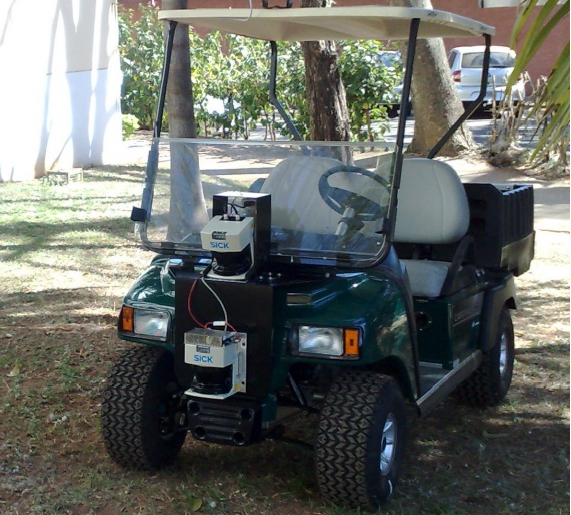
\includegraphics[width=8cm,height=7cm]{images/carina_1.png}
	 	\caption{CaRINA I - Carro elétrico automatizado.}
		\fonte{LRM (divulgação)}
	 	\label{fig:carina}
 	%\end{minipage}
\end{figure}

%Para realizar os
%testes e avaliar o desempenho do sistema proposto teremos à disposição o veículo
%CaRINA I, que já possui integrada uma câmera de vídeo estéreo e um dispositivo
%de localização GPS com bússola, bem como outros dispositivos sensores e
%atuadores de controle do veículo. O veículo CaRINA I é o mais adaptado para
%ambientes externos não estruturados (off-road) a que pretendemos aplicar. Já o
%veículo CaRINA II está mais focado para ambientes urbanos (vias e estradas
%urbanas).

A primeira etapa do projeto consiste no levantamento de todos os pontos críticos
do sistema proposto, após esta etapa serão avaliadas as técnicas mais acessíveis
que são adequadas para o tratamento de cada ponto crítico. Será levado em conta
prioritariamente o que já vem sendo trabalhado no laboratório, a fim de promover
a integração das tecnologias já dominadas pelo grupo.
% Para a programação serão utilizadas as bibliotecas OpenCV\foot{OpenCV -
% http://opencv.willowgarage.com/} e PCL\foot{PCL - http://pointclouds.org} como
% ferramentas centrais.
% , podendo vir a ser utilizado o framework ROS\foot{ROS - http://www.ros.org}
% para a integração destas ferramentas.
Para a localização global será aplicada basicamente a utilização de GPS e
bússola. Como o destino também será dado em forma de informação de posição de
GPS esta questão não é tão crítica para esse projeto. A localização é bastante
afetada por ruídos dos sensores, principalmente aqueles que fornecem informações
de odometria. Dependendo da aplicação pode ser desnecessário considerar uma
localização espacial precisa do veículo, apenas que o mesmo seja capaz de chegar
no seu destino eficazmente. Por se tratar de um ambiente externo e não
estruturado, sua navegação permite uma certa liberdade de movimentos dentro de
um perímetro onde haja um caminho factível, preferencialmente buscando um
caminho próximo do ótimo, como é o caso deste trabalho. Desta forma, o erro
associado ao posicionamento por GPS não está sendo considerado crítico.

%Em relação ao sistema de controle do veículo está sendo considerada uma 
%abordagem primeiramente deliberativa, onde as trajetórias serão planejadas de acordo com 

A abordagem da visão computacional se insere como principal fonte de informação
sensorial do ambiente no contexto deste projeto. Inicialmente serão estudados e
trabalhados algoritmos para a criação do mapa de disparidade a partir do par de
imagens obtidas da câmera estéreo.
% Neste processo, o algoritmo deverá ter um compromisso de desempenho entre a
% qualidade do mapa de disparidade/profundidade e a performance em termos de
% tempo de processamento.
A partir do mapa de disparidade será elaborado um mapa de navegabilidade, que
representa as regiões navegáveis (seguras) e regiões não navegáveis (obstáculos
e regiões a evitar) em frente ao veículo. O mapa final gerado será utilizado em
conjunto com as informações de posição atual e de destino (GPS e bússola), a fim
de realizar a navegação do veículo.


A primeira abordagem na construção de mapas de navegabilidade a partir de
informações visuais será pesquisada a viabilidade de se gerar mapas de
profundidade menos densos a cada instante de tempo com o propósito de reduzir o
custo computacional desta técnica. Para tal pretende-se utilizar a estratégia de
foco de atenção, onde apenas uma região de maior interesse é analisada a cada
momento. Como o veículo está em movimento o foco de atenção é constantemente
atualizado, com isso espera-se obter um mapeamento do ambiente de forma
incremental suficiente para o planejamento da navegação.

Serão desenvolvidos estudos relacionados à aplicação de técnicas de campos
potenciais e de algoritmos derivados do VFH, a fim de realizar o planejamento e
controle da navegação do veículo autônomo. Além destes estudos, também serão
desenvolvidos estudos relativos ao uso de Redes Neurais Artificiais (RNAs) para
o controle da navegação do veículo, conforme proposto no trabalho dos
RoBombeiros. Ambas as técnicas, VFH e RNAs, são adequadas para uma navegação
baseada em um ponto/orientação de destino (fornecido pelas coordenadas GPS).
Assim, será possível inclusive comparar o desempenho e resultados obtidos com
cada uma destas técnicas, permitindo uma melhor avaliação e escolha do melhor
método a ser adotado no veículo autônomo.
Nestas duas abordagens serão consideradas como parâmetro de entrada as
informações tridimensionais do mapa de navegabilidade. Além disto, também serão
necessários estudos que visam identificar, a partir das imagens da câmera
estéreo, o plano de referência de base (chão), seus desníveis e impedimentos,
classificando-os como elementos transponíveis ou não. 

%Elemento que também é
%parâmetro para o planejamento, controle e estratégia da navegação.

%Para o desenvolvimento do sistema de navegação autônoma do veículo será
%utilizada a ferramenta Player-Stage\foot{Player Project e Player-Stage -
%http://www.willowgarage.com/pages/software/player e
%http://playerstage.sourceforge.net}, que já vem sendo adotada junto ao LRM (Wolf
%et al., 2009).
%Esta ferramenta permite desenvolver simulações dos robôs e veículos móveis
%baseadas no uso de sensores e atuadores virtuais equivalentes aos disponíveis no
%veículo. O software Player também provê ferramentas para o acesso aos
%dispositivos de hardware do robô, oferecendo uma interface (API) de alto nível
%para acesso aos drivers de dispositivos, como o GPS, a bússola, e os
%controladores dos motores do veículo. Esta ferramenta tem permitido um maior
%reaproveitamento de código e maior produtividade no desenvolvimento de
%aplicações robóticas junto ao LRM.

\textbf{O método de trabalho proposto neste trabalho consiste na execução
continuada das seguintes etapas:}

\begin{itemize}
\item Coleta de dados (ambiente real)
\item Simulação e análise com os dados coletados
\item Verificação (comportamento) em ambiente simulado 
\item Validação (ambiente real)
\end{itemize}


\subsection{Simulação}

Para este trabalho a simulação desempenhará papel essencial nos testes e na
avaliação das técnicas a serem utilizadas. Para tal será utilizada a plataforma
ROS\foot{ROS - Robotic Operating System - http://www.ros.org} que possui o
simulador físico 3D Gazebo. Esta plataforma está sendo considerara por estar
sendo adotada por diversos grupos de pesquisa na área da robótica. É uma
plataforma \textit{Open Source} que também tem servido de repositório para
compartilhar implementações de algoritmos propostos pela comunidade científica,
assim como \textit{drivers} de acesso aos dispositivos físicos, como sensores e
até mesmo plataformas robóticas completas (ex.
PR2\foot{PR2 - Personal Robot 2 - http://www.willowgarage.com}).

%OSORIO
%> Podia detalhar um pouco mais o ROS, descrevendo as facilidades que oferece,
% os recursos (log, drivers, simulação no gazebo, etc). Ficou muito resumido 
% e compacta esta parte. Não tem nem uma imagem do Carina I virtual !
% Imagino que esteja nos planos escrever mais sobre isto, mas desde já fica o
% pedido de mais detalhes aqui.

% A simulação neste contexto tem como principais vantagens e desvantagens:
\textbf{O uso da simulação no contexto deste projeto tem como principais aspectos:}

\begin{itemize}
\item Maior repetibilidade dos experimentos;
\item Replicação dos experimentos (e sem necessidade do equipamento físico);
\item Versatilidade (ex. troca de componentes, sensores, cenário, etc.).
\item Segurança (experimentos preliminares sem comprometer os equipamentos)
\end{itemize}

\textbf{Como desvantagens, a simulação pode ter os seguintes aspectos:}

\begin{itemize}
\item A modelagem dos cenários é custosa (tempo);
\item Não reflete fielmente a realidade.
\end{itemize}


A modelagem do sistema em um ambiente virtual é um passo fundamental para
executar experimentos em um simulador. Os experimentos em simulação podem ser
replicados e repetidos mais facilmente, desta forma, uma maior quantidade de
dados pode ser extraída para análises e verificação do comportamento dos
algoritmos. A maioria dos algoritmos utilizados no contexto da robótica móvel
autônoma requerem uma parametrização e um refino de diversos parâmetros para se
adequarem às necessidades da aplicação. Este refino está diretamente associado
aos comportamentos desejados que devem ser testados. Com o uso de simulação
estes parâmetros e seus efeitos podem ser melhor observados antes de se levar o
experimento para o ambiente real.

Para a plataforma CaRINA I que será utilizada já foram descritos os modelos de
simulação, do veículo e de alguns cenários de testes (\fig{fig:model},
\fig{fig:gazebo}).

\begin{figure}[ht]
	\begin{minipage}[b]{0.4\linewidth}
	    \centering
	    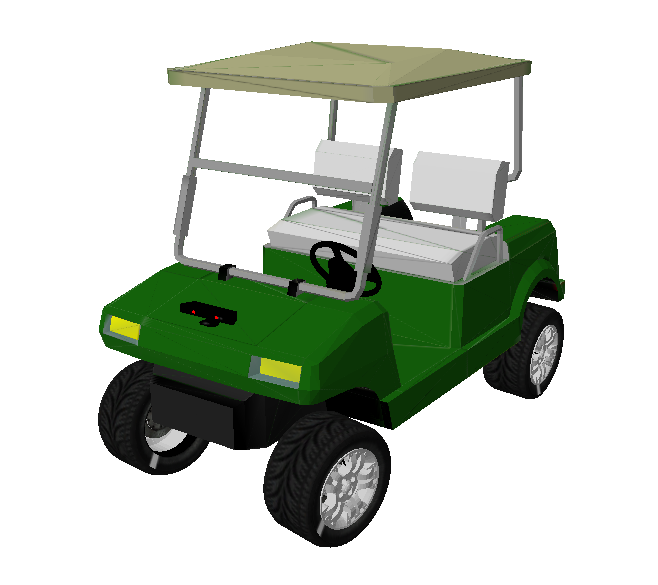
\includegraphics[width=8cm]{modelo_carina/carina_rviz_fundo_branco_sem_grid.png}
	 	\caption{CaRINA I - modelo virtual}
	 	\label{fig:model}
	\end{minipage}
	\hspace{1cm}
	\begin{minipage}[b]{0.4\linewidth}
	    \centering
	    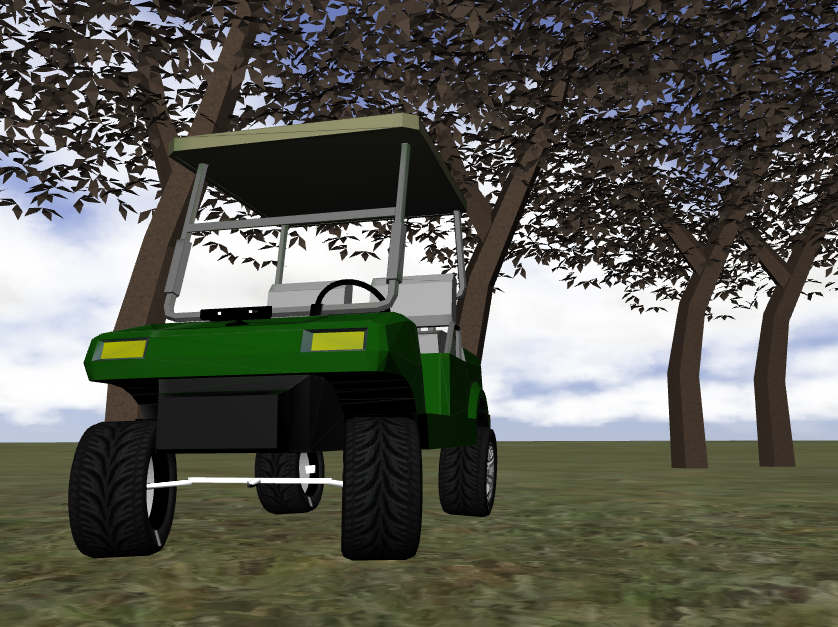
\includegraphics[width=8cm]{modelo_carina/carina_gazebo_frente_fundo.png}
	 	\caption{CaRINA I - cenário de ambiente não estruturado}
	 	\label{fig:gazebo}
	\end{minipage}
\end{figure}

Para a modelagem de robôs na plataforma ROS é utilizada uma linguagem para a
descrição chamada URDF (\textit{Unified Robot Description Format}). O URDF é
uma linguagem de descrição em XML onde basicamente são informadas os componentes,
sensores e relações entre as partes do robô, cada qual tendo um sistema de
coordenadas próprio. Estas relações podem ser móveis ou fixas, determinando
assim transformações entre cada sistema de coordenada. Toda informação sensorial
e de controle está associada a origem do seu sistema de coordenadas.

%\subsection{Model Description}
%
%For modelling robots in ROS there is a formal description languange called
% URDF.
%URDF is a language in XML formatting that is used basically to describe the
%transform relations between the robot's coordinates frames. Each moving part of
%the robot and each sensor has its own reference coordinate frame for the
%generated data. In ROS, all coordinate systems are kept by a component called
% TF that is responsible to provide the transformed coordinates from one frame to
%another. This is an important concept and framework provided by ROS, where data
%can be generated and manipulated within its own fixed coordinate frame and then
%transformed easily to others coordinates frames for combining sensors data and
%robot states. Since these transforms must be done from one frame to another,
%uniquely and in any order, the robot coordinates frames are represented by a
%tree in a parent-child relation (\fig{fig:tf},\fig{fig:tree}).

%\begin{figure}[h!]
%	\begin{minipage}[b]{0.5\linewidth}
%	    \centering
%	   
%	    %
%	    %
%	    %
	    % 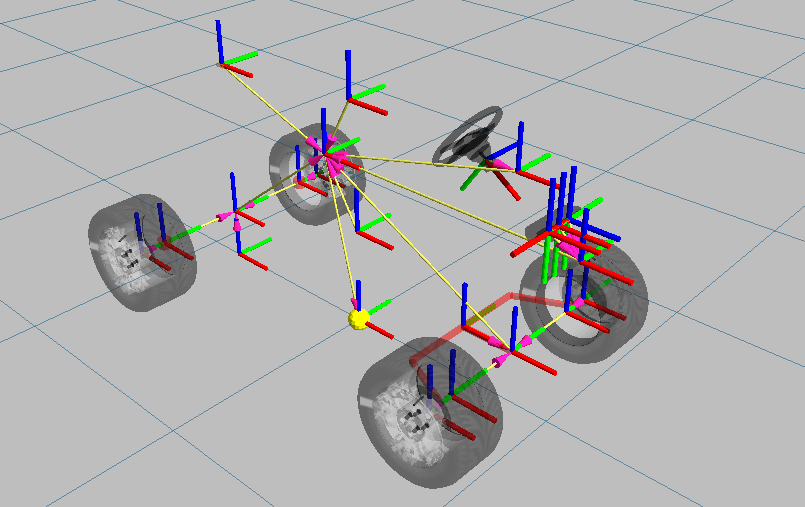
\includegraphics[width=6cm]{modelo_carina/carina_tf_side_wheels_transp.png}
%	 	\caption{Sistemas de coordenadas de referência (TF)}
%	 	\label{fig:tf}
%	\end{minipage}
%	\begin{minipage}[b]{0.5\linewidth}
%	    \centering
%	    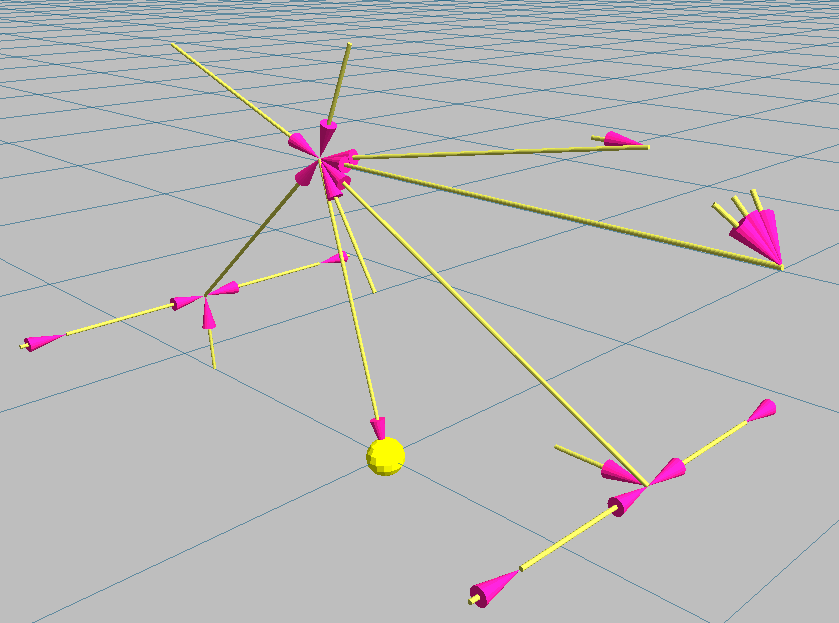
\includegraphics[width=6cm]{modelo_carina/carina_tf_side_no_axis.png}
%	 	\caption{Representação em árvore}
%	 	\label{fig:tree}
%	\end{minipage}	
%\end{figure}

%Most physical simulation libraries uses the concept of links and joints
%to describe physical relations of the structures of a body. A joint describe
%a relation between links and both can present physical properties like friction
%coefficients, elasticity and masses. These links and joint represent physical
%relations and mechanical structures of the robot like arms, wheels and its
%axels and so on. To describe links and joints relations, a graph representation
%would be more suited and this makes the URDF tree structure a little limiting
%to fully describe the model.

%Gazebo has its own XML description language called SDF to model scenarios and
%robots with its physics parameters. SDF share some compatibility with URDF and
%URDF can be extended with Gazebo specific tags, this way the same robot
%description can be shared between ROS and Gazebo. The Gazebo specific modelling
%descriptions are used to plug sensors and controllers to the virtual model and
%also allows describing some mechanical restrictions not permited by the tree
%structure of URDF, like the case in the CaRINA model where the Ackermann
%Geometry was modelled (\fig{fig:ackermann}).

%\begin{figure}[h!]
%	\begin{minipage}[b]{1\linewidth}
%	    \centering
%	    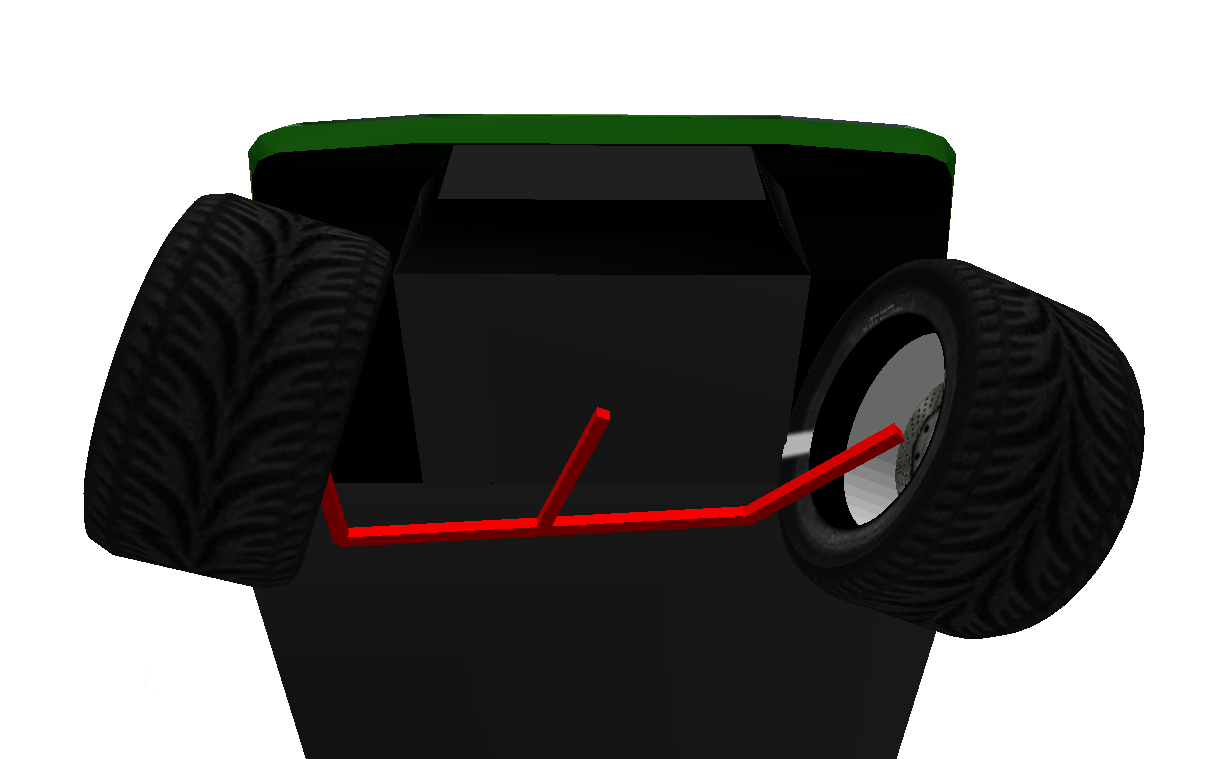
\includegraphics[width=6cm]{modelo_carina/carina_rviz_steering.png}
%	 	\caption{Ackermann steering geometry modelled in simulation}
%	 	\label{fig:ackermann}
%	\end{minipage}
%\end{figure}

%We also put on the virtual model a suspension mechanism independant on each
%wheel. Since our intentions are not to simulate the mechanical behaviour of the
%car itself but our autonomous navigation systems, the suspension is an
%aproximation model just enought to enable us to simulate on uneven terrains
%avoiding the kicking collision effect with the ground caused by the ridgid body
%physics simulation and keeping the four wheels in contact with the ground to
%avoid loss of traction, splipages and unstable poses of the vehicle that
%diverges from real situations. One other effect desired from the simulated
%suspension is the balancing of the vehicle when bending, accelareting and
%breaking, that will have a direct effect on the sensors reading and be more
%close to real situations. This give us a better simulated IMU data with a more
%realistic associated noise (\fig{fig:uneven}).

%\begin{figure}[ht]
%	\begin{minipage}[b]{1\linewidth}
%	    \centering
%	    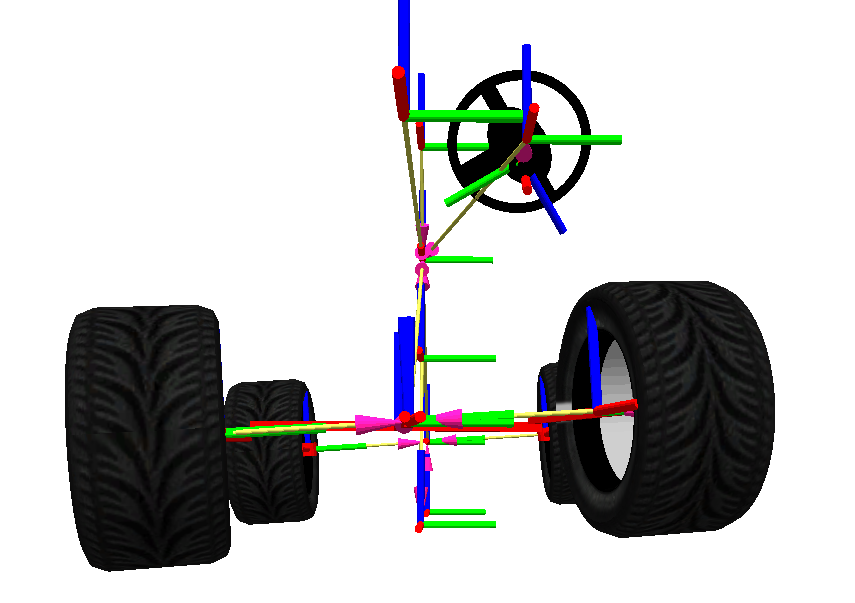
\includegraphics[width=8cm]{modelo_carina/carina_rviz_uneven_susp.png}
%	 	\caption{Suspension effect on an uneven terrain}
%	 	\label{fig:uneven}
%	\end{minipage}
%\end{figure}

\subsection{Arquitetura}

Para o desenvolvimento do sistema e execução no ambiente real também será
utilizada a plataforma ROS, pois ela foi elaborada tendo como um dos propósitos
a padronização de uma interface para dispositivos reais e simulados. Isto
permite o desenvolvimentos dos algoritmos de forma independente da fonte dos
dados.

A arquitetura do sistema de navegação será baseado no modelo geral do ROS
conforme a \fig{fig:arq}.

%OSORIO

%> O ideal é ter figuras em Português, evitando textos em inglês (inclusive na
% tabela abaixo na figira onde apresenta a notação adotada)

%> Seria necessário um texto comentando e detalhando o que representa esta
% figura e seus componentes.

%\vspace{1cm}

%ao mesmo tempo que o custo computacional associado

\begin{figure}[!h]
  	\centering
%	\begin{minipage}[b]{1.0\linewidth}
	    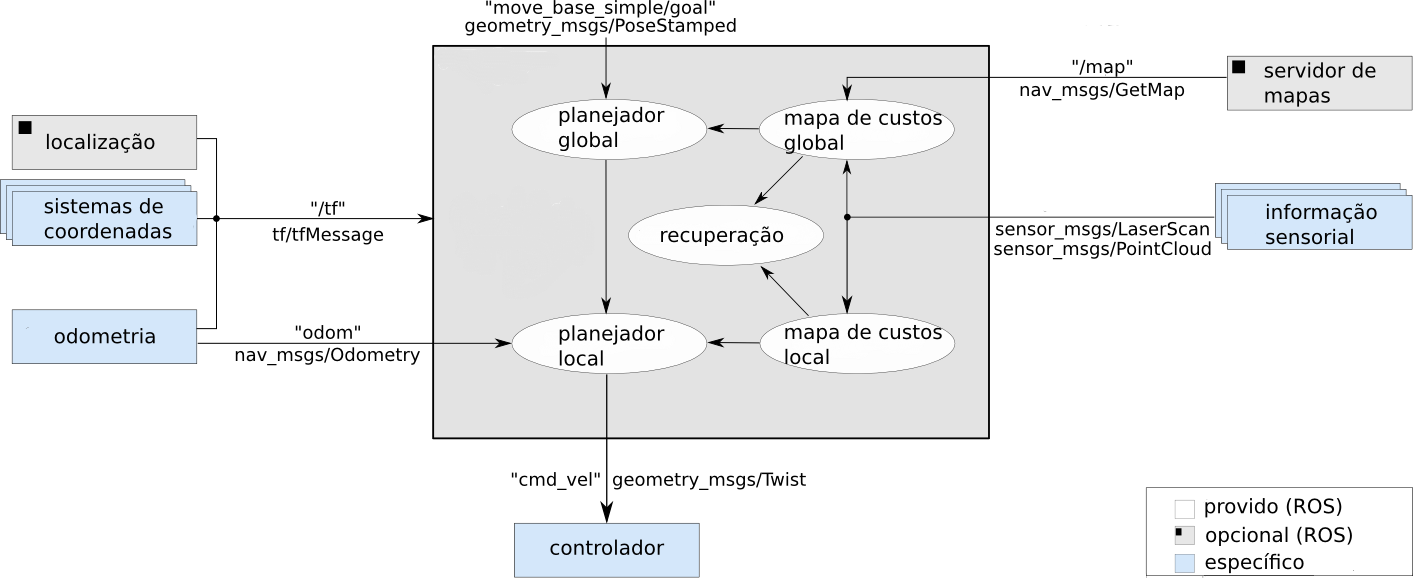
\includegraphics[width=\textwidth,height=8cm]{images/overview_tf_pt.png}
	 	\caption{Arquitetura geral do sistema de navegação.}
		\fonte{adaptado de: www.ros.org}
	 	\label{fig:arq}
% 	\end{minipage}
\end{figure}

Esta arquitetura se baseia em um comportamento deliberativo em relação ao
mapeamento global e um comportamento reativo associado ao mapeamento local. O
serviço de mapa deve fornecer informações de ocupação do espaço, geralmente
discretizado em livre, ocupado e desconhecido. Estes atributos são utilizados no
cálculo dos custos utilizado pelo algoritmo de geração de trajetória. Estes
custos são mantidos pelos mapas de custos e atualizados de acordo com as
informações sensoriais que são constantemente analisadas. 

Nesta arquitetura os componentes específicos dizem respeito ao veículo
e sensores utilizados. Já os componentes providos pela plataforma ROS requerem
as devidas parametrizações e a escolha dos algoritmos adequados para o problema
que ainda estão sendo estudados.

%Os algoritmos de geração de trajetória baseados em amostras tem sido adotado em
%robótica móvel com maior ênfase principalmente pela aplicabilidade prática,
% este tipo de abordagem leva em consideração a cinemática do veículo gerando
%trajetórias realistas com custo computacional baixo \cite{ompl}.

%Por se tratar de uma plataforma aberta todos componentes podem ser customizado
% e adaptados 
%Para a localização já foi 

%A primeira tarefa realizada no projeto foi a modelage do veículo para
%utilização no simulador, esta modelagem contempla a cinemática do veículo no
% modelo Ackerman, onde a angulação das rodas dianteiras são independentes em relação ao
%ângulo de esterçamento do veículo \fig{fig:ackerman}. Esta modelagem também
%contempla os sensores presentes no veículo real que serão utilizados no
% projeto.

%Uma etapa necessária para a navegação é a odometria do veículo, esta odometria
%foi implementada baseando-se nas informações provenientes da contagem de
%rotações da roda juntamente com a medição do angulo de giro da barra de
% direção.




\section{Forma de Análise dos Resultados}

Os resultados serão analisados comparativamente com as soluções já desenvolvidas
no LRM e em comparação com projetos semelhantes e relacionados. Além disto,
serão avaliadas e comparadas as diferentes abordagens adotadas neste estudo,
como por exemplo, comparando a abordagem baseada em VFH com RNAs. Outro quesito
a ser avaliado é o desempenho geral do sistema, onde serão realizadas medições e
avaliações dos tempos de processamento e do desempenho alcançados.

%A adaptabilidade e robustez final do resultado para as áreas de interesse e aplicação citadas nesta
%proposta irá indicar o grau de sucesso atingido. As necessidades de melhorias e a delineação de
%avanços que devem ser alcançados poderão servir de base para novos projetos, constituindo um
%avanço na prospecção tecnológica para o desenvolvimento de um sistema eficiente e robusto de
%navegação autônoma.

A métrica quantitativa mais utilizada para este tipo de sistema são as
frequências em que se permite executar os algoritmos. No caso de imagens a taxa
é dada em FPS (imagens por segundo). Estas taxas tem como principal papel
expressar os resultados de forma que possam ser utilizados para verificar se é
possível construir um sistema tempo real. Uma outra métrica relevante para
categorizar os métodos é uma avaliação qualitativa de quão paralelizável é o
algoritmo utilizado. Esta métrica geralmente acaba sendo apresentada de forma
implícita na descrição da estrutura do algoritmo.

%Para análises estatísticas geralmente são necessários critérios  

%OSORIO
% A validação por simulação permite também gerar situações mais variadas e
% avaliar os limites e capacidades do sistema proposto: variando 
% a densidade/quantidade de obstáculos presentes no ambiente; avaliando a
% quantidade de colisões que podem vir a ocorrer em determinadas situações; 
% verificando em que situações um obstáculo pode vir a não ser detectado; e
% assim por diante.

A primeira etapa consistem em avaliar o sistema em ambiente simulado. A
validação por simulação permite gerar diversas situações desejadas para testar
variados comportamentos sem a necessidade de criá-las no ambiente real, o que
dependendo do cenário pode ser arriscado. A simulação permite maior controle
sobre o ambiente permitindo cenários mais propícios e menos propícios afim de
verificar a robustez do sistema. As análises em ambiente real serão comparadas
com os testes efetuados em simulação permitindo uma avaliação do desempenho,
tanto da qualidade das trajetórias geradas como a capacidade de desvio de
obstáculos.

%OSORIO
%> As "considerações finais" deste capítulo podem ser uma lista da principais
%contribuições esperadas deste trabalhos descritas sobre a forma de uma lista de
% itens.

\section{Contribuições Esperadas}

As principais contribuições acadêmico-científicas esperadas deste trabalho são: 

\begin{enumerate}[i.]

\item adaptação e aperfeiçoamento dos algoritmos para a geração em “tempo real”
de mapas de disparidade, obtendo estes mapas a partir de um par de imagens
capturadas pela câmera estéreo;

\item proposta e desenvolvimento de algoritmos para a obtenção de mapas locais
de navegabilidade com informações espaciais (3D), onde o espaço tridimensional
será dividido em regiões e estas regiões serão identificadas como sendo
navegáveis ou não navegáveis;

\item aperfeiçoamento de técnicas para a navegação baseada no uso de GPS,
bússola e mapas locais de navegabilidade, onde as pesquisas previamente
desenvolvidas para detectar e desviar de obstáculos com o uso de mapas 2D, serão
estendidas a fim de trabalhar com mapa de navegabilidade/ocupação em 3D. Deste
trabalho resultará um sistema com possibilidade de aplicação prática em
importantes tarefas de navegação autônoma, como por exemplo, em sistemas
voltados para aplicações agrícolas e em sistema de combate a incêndio em
florestas, tarefas estas que podem ser perigosas para o ser humano (por exemplo,
exposição prolongada aos produtos químicos de defensivos agrícolas, e
combate/contato direto com fumaça e incêndios).

\end{enumerate}

\section{Objetivos Específicos}

Os principais objetivos específicos deste projeto de mestrado, que se apresentam
como um desdobramento do objetivo geral descrito acima, são:

\begin{itemize}

\item Extração de referenciais a partir de um par de câmeras, constituindo um
sistema de visão binocular (estéreo);

\item Propor melhorias nos algoritmos de geração do mapa de disparidade, obtido
a partir das imagens estéreo;

\item Gerar um mapa de navegabilidade local a partir de informações visuais;
%,
%que possa ser adaptado a algoritmos de planejamento e controle de navegação
%autônoma;

\item Desenvolver um mecanismo de navegação autônoma, baseado nas informações de
GPS, Bússola e do Sistema de Visão, capaz de desviar de obstáculos e dirigir o
veículo até um destino determinado de forma robusta e eficiente;

\item Fazer uso dos conhecimentos prévios de trabalhos desenvolvidos no
laboratório e contribuir para a consolidação de tecnologias capazes de atribuir
navegabilidade autônoma a veículos de diversas naturezas para fins práticos;

\item Aplicação e avaliação do sistema de navegação autônoma em um veículo real
em ambiente externo não estruturado.

\end{itemize}

%2012-10-15 Revisar
\section{Materiais e Métodos}

Este trabalho será desenvolvido junto ao LRM\foot{LRM - Laboratório de Robótica
Móvel do ICMC/USP - http://www.lrm.icmc.usp.br} – Laboratório de Robótica Móvel
do ICMC/USP. Diversos trabalhos relacionados ao desenvolvimento de veículos
autônomos e robôs móveis inteligentes vêm sendo pesquisados e desenvolvidos
junto a este laboratório, destacando-se, a pesquisa e uso de sistemas de
navegação baseados em visão computacional.
% Atualmente, o Laboratório conta com uma parceria estabelecida com a empresa
% Jacto S/A\foot{Grupo Jacto - http://www.jacto.com.br} (equipamentos agrícolas)
% para o desenvolvimento de um sistema autônomo de navegação de veículos em
% ambientes agrícolas.
O LRM possui atualmente duas plataformas de teste para aplicações de veículos
móveis autônomos que foram adquiridas pelo INCT-SEC: os veículos CaRINA I e
CaRINA II\foot{CaRINA - Carro Robótico Inteligente para Navegação Autônoma -
http://www.lrm.icmc.usp.br}
% (fig. 3.1).
% Também, possui robôs e plataformas móveis de pequeno porte.
Para realizar as atividades de validação em ambiente real será utilizada a
plataforma CaRINA I (\fig{fig:carina}) que possui a automatização dos seus controles de frenagem,
aceleração e esterçamento. O veículo CaRINA I é o mais adaptado para ambientes
externos não estruturados (\textit{off-road}), já o veículo CaRINA II é mais
focado para ambientes urbanos (vias e estradas urbanas).

\vspace{0.5cm}
\begin{figure}[!h]
  	\centering
	%\begin{minipage}[b]{0.33\linewidth}
	    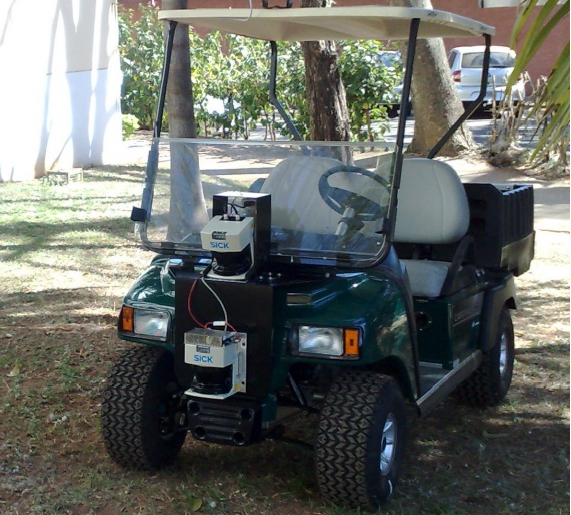
\includegraphics[width=8cm,height=7cm]{images/carina_1.png}
	 	\caption{CaRINA I - Carro elétrico automatizado.}
		\fonte{LRM (divulgação)}
	 	\label{fig:carina}
 	%\end{minipage}
\end{figure}

%Para realizar os
%testes e avaliar o desempenho do sistema proposto teremos à disposição o veículo
%CaRINA I, que já possui integrada uma câmera de vídeo estéreo e um dispositivo
%de localização GPS com bússola, bem como outros dispositivos sensores e
%atuadores de controle do veículo. O veículo CaRINA I é o mais adaptado para
%ambientes externos não estruturados (off-road) a que pretendemos aplicar. Já o
%veículo CaRINA II está mais focado para ambientes urbanos (vias e estradas
%urbanas).

A primeira etapa do projeto consiste no levantamento de todos os pontos críticos
do sistema proposto, após esta etapa serão avaliadas as técnicas mais acessíveis
que são adequadas para o tratamento de cada ponto crítico. Será levado em conta
prioritariamente o que já vem sendo trabalhado no laboratório, a fim de promover
a integração das tecnologias já dominadas pelo grupo.
% Para a programação serão utilizadas as bibliotecas OpenCV\foot{OpenCV -
% http://opencv.willowgarage.com/} e PCL\foot{PCL - http://pointclouds.org} como
% ferramentas centrais.
% , podendo vir a ser utilizado o framework ROS\foot{ROS - http://www.ros.org}
% para a integração destas ferramentas.
Para a localização global será aplicada basicamente a utilização de GPS e
bússola. Como o destino também será dado em forma de informação de posição de
GPS esta questão não é tão crítica para esse projeto. A localização é bastante
afetada por ruídos dos sensores, principalmente aqueles que fornecem informações
de odometria. Dependendo da aplicação pode ser desnecessário considerar uma
localização espacial precisa do veículo, apenas que o mesmo seja capaz de chegar
no seu destino eficazmente. Por se tratar de um ambiente externo e não
estruturado, sua navegação permite uma certa liberdade de movimentos dentro de
um perímetro onde haja um caminho factível, preferencialmente buscando um
caminho próximo do ótimo, como é o caso deste trabalho. Desta forma, o erro
associado ao posicionamento por GPS não está sendo considerado crítico.

%Em relação ao sistema de controle do veículo está sendo considerada uma 
%abordagem primeiramente deliberativa, onde as trajetórias serão planejadas de acordo com 

A abordagem da visão computacional se insere como principal fonte de informação
sensorial do ambiente no contexto deste projeto. Inicialmente serão estudados e
trabalhados algoritmos para a criação do mapa de disparidade a partir do par de
imagens obtidas da câmera estéreo.
% Neste processo, o algoritmo deverá ter um compromisso de desempenho entre a
% qualidade do mapa de disparidade/profundidade e a performance em termos de
% tempo de processamento.
A partir do mapa de disparidade será elaborado um mapa de navegabilidade, que
representa as regiões navegáveis (seguras) e regiões não navegáveis (obstáculos
e regiões a evitar) em frente ao veículo. O mapa final gerado será utilizado em
conjunto com as informações de posição atual e de destino (GPS e bússola), a fim
de realizar a navegação do veículo.


A primeira abordagem na construção de mapas de navegabilidade a partir de
informações visuais será pesquisada a viabilidade de se gerar mapas de
profundidade menos densos a cada instante de tempo com o propósito de reduzir o
custo computacional desta técnica. Para tal pretende-se utilizar a estratégia de
foco de atenção, onde apenas uma região de maior interesse é analisada a cada
momento. Como o veículo está em movimento o foco de atenção é constantemente
atualizado, com isso espera-se obter um mapeamento do ambiente de forma
incremental suficiente para o planejamento da navegação.

Serão desenvolvidos estudos relacionados à aplicação de técnicas de campos
potenciais e de algoritmos derivados do VFH, a fim de realizar o planejamento e
controle da navegação do veículo autônomo. Além destes estudos, também serão
desenvolvidos estudos relativos ao uso de Redes Neurais Artificiais (RNAs) para
o controle da navegação do veículo, conforme proposto no trabalho dos
RoBombeiros. Ambas as técnicas, VFH e RNAs, são adequadas para uma navegação
baseada em um ponto/orientação de destino (fornecido pelas coordenadas GPS).
Assim, será possível inclusive comparar o desempenho e resultados obtidos com
cada uma destas técnicas, permitindo uma melhor avaliação e escolha do melhor
método a ser adotado no veículo autônomo.
Nestas duas abordagens serão consideradas como parâmetro de entrada as
informações tridimensionais do mapa de navegabilidade. Além disto, também serão
necessários estudos que visam identificar, a partir das imagens da câmera
estéreo, o plano de referência de base (chão), seus desníveis e impedimentos,
classificando-os como elementos transponíveis ou não. 

%Elemento que também é
%parâmetro para o planejamento, controle e estratégia da navegação.

%Para o desenvolvimento do sistema de navegação autônoma do veículo será
%utilizada a ferramenta Player-Stage\foot{Player Project e Player-Stage -
%http://www.willowgarage.com/pages/software/player e
%http://playerstage.sourceforge.net}, que já vem sendo adotada junto ao LRM (Wolf
%et al., 2009).
%Esta ferramenta permite desenvolver simulações dos robôs e veículos móveis
%baseadas no uso de sensores e atuadores virtuais equivalentes aos disponíveis no
%veículo. O software Player também provê ferramentas para o acesso aos
%dispositivos de hardware do robô, oferecendo uma interface (API) de alto nível
%para acesso aos drivers de dispositivos, como o GPS, a bússola, e os
%controladores dos motores do veículo. Esta ferramenta tem permitido um maior
%reaproveitamento de código e maior produtividade no desenvolvimento de
%aplicações robóticas junto ao LRM.

\textbf{O método de trabalho proposto neste trabalho consiste na execução
continuada das seguintes etapas:}

\begin{itemize}
\item Coleta de dados (ambiente real)
\item Simulação e análise com os dados coletados
\item Verificação (comportamento) em ambiente simulado 
\item Validação (ambiente real)
\end{itemize}


\subsection{Simulação}

Para este trabalho a simulação desempenhará papel essencial nos testes e na
avaliação das técnicas a serem utilizadas. Para tal será utilizada a plataforma
ROS\foot{ROS - Robotic Operating System - http://www.ros.org} que possui o
simulador físico 3D Gazebo. Esta plataforma está sendo considerara por estar
sendo adotada por diversos grupos de pesquisa na área da robótica. É uma
plataforma \textit{Open Source} que também tem servido de repositório para
compartilhar implementações de algoritmos propostos pela comunidade científica,
assim como \textit{drivers} de acesso aos dispositivos físicos, como sensores e
até mesmo plataformas robóticas completas (ex.
PR2\foot{PR2 - Personal Robot 2 - http://www.willowgarage.com}).

%OSORIO
%> Podia detalhar um pouco mais o ROS, descrevendo as facilidades que oferece,
% os recursos (log, drivers, simulação no gazebo, etc). Ficou muito resumido 
% e compacta esta parte. Não tem nem uma imagem do Carina I virtual !
% Imagino que esteja nos planos escrever mais sobre isto, mas desde já fica o
% pedido de mais detalhes aqui.

% A simulação neste contexto tem como principais vantagens e desvantagens:
\textbf{O uso da simulação no contexto deste projeto tem como principais aspectos:}

\begin{itemize}
\item Maior repetibilidade dos experimentos;
\item Replicação dos experimentos (e sem necessidade do equipamento físico);
\item Versatilidade (ex. troca de componentes, sensores, cenário, etc.).
\item Segurança (experimentos preliminares sem comprometer os equipamentos)
\end{itemize}

\textbf{Como desvantagens, a simulação pode ter os seguintes aspectos:}

\begin{itemize}
\item A modelagem dos cenários é custosa (tempo);
\item Não reflete fielmente a realidade.
\end{itemize}


A modelagem do sistema em um ambiente virtual é um passo fundamental para
executar experimentos em um simulador. Os experimentos em simulação podem ser
replicados e repetidos mais facilmente, desta forma, uma maior quantidade de
dados pode ser extraída para análises e verificação do comportamento dos
algoritmos. A maioria dos algoritmos utilizados no contexto da robótica móvel
autônoma requerem uma parametrização e um refino de diversos parâmetros para se
adequarem às necessidades da aplicação. Este refino está diretamente associado
aos comportamentos desejados que devem ser testados. Com o uso de simulação
estes parâmetros e seus efeitos podem ser melhor observados antes de se levar o
experimento para o ambiente real.

Para a plataforma CaRINA I que será utilizada já foram descritos os modelos de
simulação, do veículo e de alguns cenários de testes (\fig{fig:model},
\fig{fig:gazebo}).

\begin{figure}[ht]
	\begin{minipage}[b]{0.4\linewidth}
	    \centering
	    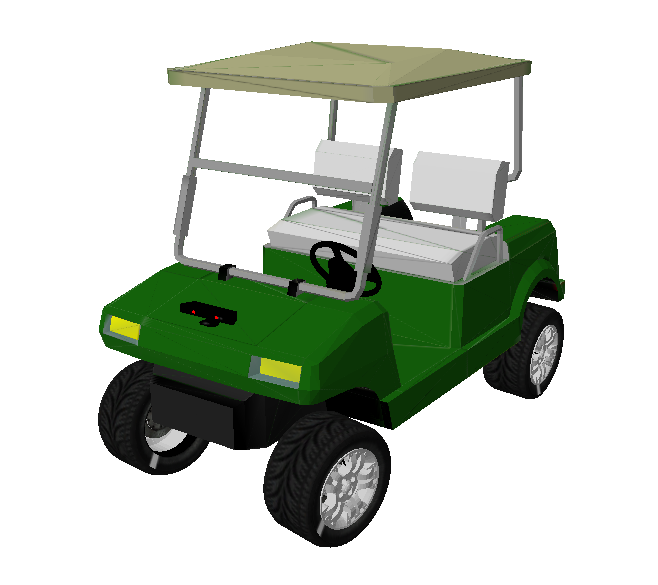
\includegraphics[width=8cm]{modelo_carina/carina_rviz_fundo_branco_sem_grid.png}
	 	\caption{CaRINA I - modelo virtual}
	 	\label{fig:model}
	\end{minipage}
	\hspace{1cm}
	\begin{minipage}[b]{0.4\linewidth}
	    \centering
	    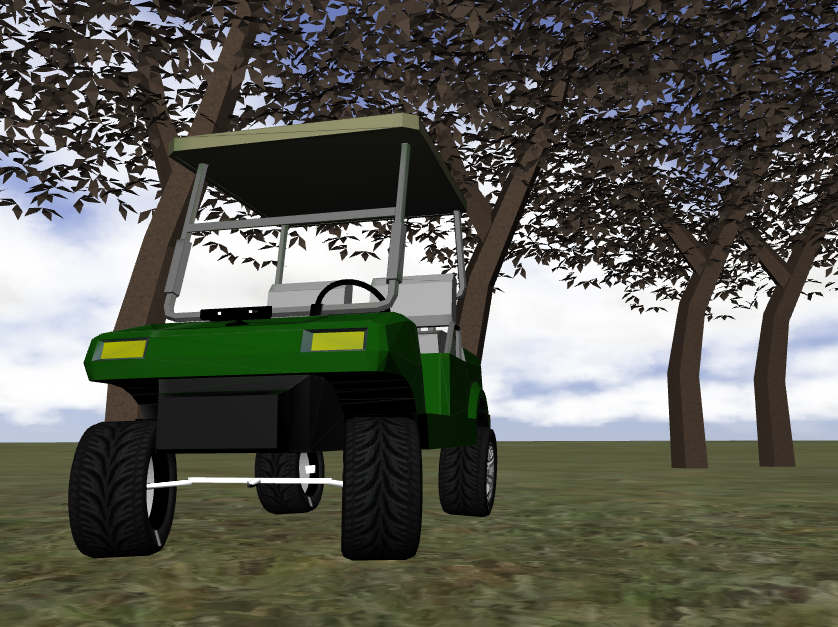
\includegraphics[width=8cm]{modelo_carina/carina_gazebo_frente_fundo.png}
	 	\caption{CaRINA I - cenário de ambiente não estruturado}
	 	\label{fig:gazebo}
	\end{minipage}
\end{figure}

Para a modelagem de robôs na plataforma ROS é utilizada uma linguagem para a
descrição chamada URDF (\textit{Unified Robot Description Format}). O URDF é
uma linguagem de descrição em XML onde basicamente são informadas os componentes,
sensores e relações entre as partes do robô, cada qual tendo um sistema de
coordenadas próprio. Estas relações podem ser móveis ou fixas, determinando
assim transformações entre cada sistema de coordenada. Toda informação sensorial
e de controle está associada a origem do seu sistema de coordenadas.

%\subsection{Model Description}
%
%For modelling robots in ROS there is a formal description languange called
% URDF.
%URDF is a language in XML formatting that is used basically to describe the
%transform relations between the robot's coordinates frames. Each moving part of
%the robot and each sensor has its own reference coordinate frame for the
%generated data. In ROS, all coordinate systems are kept by a component called
% TF that is responsible to provide the transformed coordinates from one frame to
%another. This is an important concept and framework provided by ROS, where data
%can be generated and manipulated within its own fixed coordinate frame and then
%transformed easily to others coordinates frames for combining sensors data and
%robot states. Since these transforms must be done from one frame to another,
%uniquely and in any order, the robot coordinates frames are represented by a
%tree in a parent-child relation (\fig{fig:tf},\fig{fig:tree}).

%\begin{figure}[h!]
%	\begin{minipage}[b]{0.5\linewidth}
%	    \centering
%	   
%	    %
%	    %
%	    %
	    % 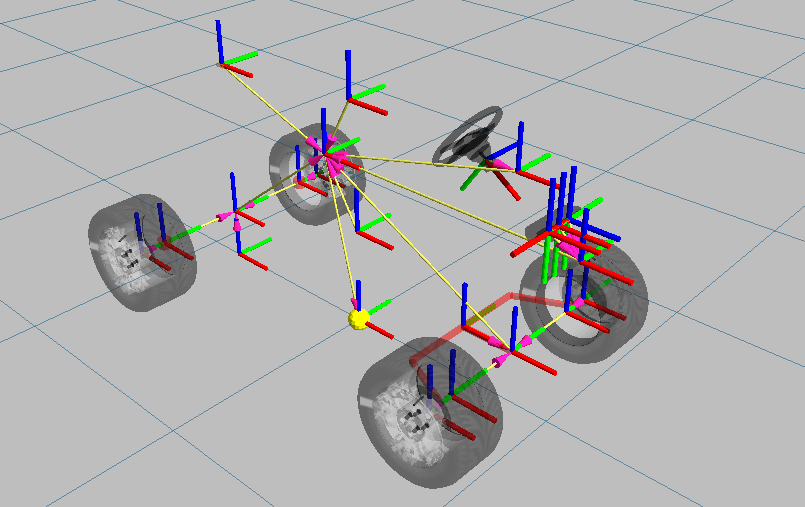
\includegraphics[width=6cm]{modelo_carina/carina_tf_side_wheels_transp.png}
%	 	\caption{Sistemas de coordenadas de referência (TF)}
%	 	\label{fig:tf}
%	\end{minipage}
%	\begin{minipage}[b]{0.5\linewidth}
%	    \centering
%	    \includegraphics[width=6cm]{modelo_carina/carina_tf_side_no_axis.png}
%	 	\caption{Representação em árvore}
%	 	\label{fig:tree}
%	\end{minipage}	
%\end{figure}

%Most physical simulation libraries uses the concept of links and joints
%to describe physical relations of the structures of a body. A joint describe
%a relation between links and both can present physical properties like friction
%coefficients, elasticity and masses. These links and joint represent physical
%relations and mechanical structures of the robot like arms, wheels and its
%axels and so on. To describe links and joints relations, a graph representation
%would be more suited and this makes the URDF tree structure a little limiting
%to fully describe the model.

%Gazebo has its own XML description language called SDF to model scenarios and
%robots with its physics parameters. SDF share some compatibility with URDF and
%URDF can be extended with Gazebo specific tags, this way the same robot
%description can be shared between ROS and Gazebo. The Gazebo specific modelling
%descriptions are used to plug sensors and controllers to the virtual model and
%also allows describing some mechanical restrictions not permited by the tree
%structure of URDF, like the case in the CaRINA model where the Ackermann
%Geometry was modelled (\fig{fig:ackermann}).

%\begin{figure}[h!]
%	\begin{minipage}[b]{1\linewidth}
%	    \centering
%	    \includegraphics[width=6cm]{modelo_carina/carina_rviz_steering.png}
%	 	\caption{Ackermann steering geometry modelled in simulation}
%	 	\label{fig:ackermann}
%	\end{minipage}
%\end{figure}

%We also put on the virtual model a suspension mechanism independant on each
%wheel. Since our intentions are not to simulate the mechanical behaviour of the
%car itself but our autonomous navigation systems, the suspension is an
%aproximation model just enought to enable us to simulate on uneven terrains
%avoiding the kicking collision effect with the ground caused by the ridgid body
%physics simulation and keeping the four wheels in contact with the ground to
%avoid loss of traction, splipages and unstable poses of the vehicle that
%diverges from real situations. One other effect desired from the simulated
%suspension is the balancing of the vehicle when bending, accelareting and
%breaking, that will have a direct effect on the sensors reading and be more
%close to real situations. This give us a better simulated IMU data with a more
%realistic associated noise (\fig{fig:uneven}).

%\begin{figure}[ht]
%	\begin{minipage}[b]{1\linewidth}
%	    \centering
%	    \includegraphics[width=8cm]{modelo_carina/carina_rviz_uneven_susp.png}
%	 	\caption{Suspension effect on an uneven terrain}
%	 	\label{fig:uneven}
%	\end{minipage}
%\end{figure}

\subsection{Arquitetura}

Para o desenvolvimento do sistema e execução no ambiente real também será
utilizada a plataforma ROS, pois ela foi elaborada tendo como um dos propósitos
a padronização de uma interface para dispositivos reais e simulados. Isto
permite o desenvolvimentos dos algoritmos de forma independente da fonte dos
dados.

A arquitetura do sistema de navegação será baseado no modelo geral do ROS
conforme a \fig{fig:arq}.

%OSORIO

%> O ideal é ter figuras em Português, evitando textos em inglês (inclusive na
% tabela abaixo na figira onde apresenta a notação adotada)

%> Seria necessário um texto comentando e detalhando o que representa esta
% figura e seus componentes.

%\vspace{1cm}

%ao mesmo tempo que o custo computacional associado

\begin{figure}[!h]
  	\centering
%	\begin{minipage}[b]{1.0\linewidth}
	    \includegraphics[width=\textwidth,height=8cm]{images/overview_tf_pt.png}
	 	\caption{Arquitetura geral do sistema de navegação.}
		\fonte{adaptado de: www.ros.org}
	 	\label{fig:arq}
% 	\end{minipage}
\end{figure}

Esta arquitetura se baseia em um comportamento deliberativo em relação ao
mapeamento global e um comportamento reativo associado ao mapeamento local. O
serviço de mapa deve fornecer informações de ocupação do espaço, geralmente
discretizado em livre, ocupado e desconhecido. Estes atributos são utilizados no
cálculo dos custos utilizado pelo algoritmo de geração de trajetória. Estes
custos são mantidos pelos mapas de custos e atualizados de acordo com as
informações sensoriais que são constantemente analisadas. 

Nesta arquitetura os componentes específicos dizem respeito ao veículo
e sensores utilizados. Já os componentes providos pela plataforma ROS requerem
as devidas parametrizações e a escolha dos algoritmos adequados para o problema
que ainda estão sendo estudados.

%Os algoritmos de geração de trajetória baseados em amostras tem sido adotado em
%robótica móvel com maior ênfase principalmente pela aplicabilidade prática,
% este tipo de abordagem leva em consideração a cinemática do veículo gerando
%trajetórias realistas com custo computacional baixo \cite{ompl}.

%Por se tratar de uma plataforma aberta todos componentes podem ser customizado
% e adaptados 
%Para a localização já foi 

%A primeira tarefa realizada no projeto foi a modelage do veículo para
%utilização no simulador, esta modelagem contempla a cinemática do veículo no
% modelo Ackerman, onde a angulação das rodas dianteiras são independentes em relação ao
%ângulo de esterçamento do veículo \fig{fig:ackerman}. Esta modelagem também
%contempla os sensores presentes no veículo real que serão utilizados no
% projeto.

%Uma etapa necessária para a navegação é a odometria do veículo, esta odometria
%foi implementada baseando-se nas informações provenientes da contagem de
%rotações da roda juntamente com a medição do angulo de giro da barra de
% direção.





\chapter{Cronograma} 
\label{cap:cronograma}

O quadro abaixo apresenta um cronograma das macro atividades deste projeto. A
execução das mesmas se dará respeitando os devidos prazos de projeto e da
pós-graduação que não estão aqui explicitados. A colocação temporal das macro
atividades estão dispostas nos períodos da sua maior concentração principal,
porém a execução das atividades se darão de forma integrada.

%\includegraphics[width=15cm,height=10cm,]{images/chrono.png}
%\centering
\includegraphics[width=16cm,height=8cm]{images/chrono.png}

\section{Participação em publicações}

%VARGAS, P. A; et al.,
\textit{Patrícia A. Vargas; Gustavo Pessin; Daniel O. Sales; Maurício A. Dias;
Rafael L. Klaser; Fernando S. Osório},
Applying Swarm Intelligence to a Garbage and Recycling Collection Problem.,
\textbf{Soft computing}, (Submetido em: Dezembro de 2012)
\\

%FERNANDES, L. C; et al.,
\textit{Leandro C. Fernandes; Jeferson R. Souza; Gustavo Pessin; Patrick Y.
Shinzato; Daniel Sales; Caio Mendes; Marcos Prado; Rafael Klaser; André Chaves
Magalhães; Daniel Pigatto; Kalinka Castelo Branco; Valdir Grassi Jr.; Fernando
S. Osório; Denis F. Wolf},
CaRINA Intelligent Robotic Car:
Architectural Design and Implementations., \textbf{Journal of System
Architecture}, (Submetido em: Janeiro de 2013)



\chapter{Resultados Esperados}
\label{cap:resultados_esperados}

Este tipo de tecnologia promove o interesse e possíveis aplicações junto à sociedade, sendo de
grande relevância à pesquisa e ao desenvolvimento de novas tecnologias nas áreas afins, a exemplo
de iniciativas como as que vêm sendo desenvolvidas em outros países (por exemplo, 
\textit{DARPA Grand/Urban Challenge}\foot{DARPA Challenge - http://www.darpa.mil/About/History/Archives.aspx}, 
\textit{ELROB}\foot{ELROB – European Robot Trial - http://www.elrob.org}, 
\textit{AUVSI/IGVC}\foot{Intelligent Ground Vehicle Competition - http://www.igvc.org}
).
Este trabalho espera contribuir no desenvolvimento de soluções para a arquitetura de um
veículo móvel autônomo robusto e seguro. Mais especificamente, este estudo estará focado na
implementação de um sistema de visão computacional para a navegação autônoma aplicável a
veículos terrestres em geral, permitindo aplicações diversas.
As principais aplicações deste sistema robótico de navegação autônoma são:

\begin{itemize}

\item
O combate à incêndios em florestas, conforme proposto nos trabalhos desenvolvidos
anteriormente por Pessin (2008);
\item 
O uso em aplicações agrícolas visando criar veículos autônomos usados para arar a terra,
semear, pulverizar e realizar a colheita em plantações, visando assim fomentar a cooperação já
estabelecida com empresas que atuam nesta área;
\item 
O uso em aplicações militares e/ou civis para o auxílio no transporte de carga e suprimentos
em ambientes não estruturados;
\item 
O transporte de cargas em locais perigosos onde a presença de um motorista possa ser
dispensada de modo a proteger sua segurança.

\end{itemize}

%\section{Forma de Análise dos Resultados}

Os resultados serão analisados comparativamente com as soluções já desenvolvidas
no LRM e em comparação com projetos semelhantes e relacionados. Além disto,
serão avaliadas e comparadas as diferentes abordagens adotadas neste estudo,
como por exemplo, comparando a abordagem baseada em VFH com RNAs. Outro quesito
a ser avaliado é o desempenho geral do sistema, onde serão realizadas medições e
avaliações dos tempos de processamento e do desempenho alcançados.

%A adaptabilidade e robustez final do resultado para as áreas de interesse e aplicação citadas nesta
%proposta irá indicar o grau de sucesso atingido. As necessidades de melhorias e a delineação de
%avanços que devem ser alcançados poderão servir de base para novos projetos, constituindo um
%avanço na prospecção tecnológica para o desenvolvimento de um sistema eficiente e robusto de
%navegação autônoma.

A métrica quantitativa mais utilizada para este tipo de sistema são as
frequências em que se permite executar os algoritmos. No caso de imagens a taxa
é dada em FPS (imagens por segundo). Estas taxas tem como principal papel
expressar os resultados de forma que possam ser utilizados para verificar se é
possível construir um sistema tempo real. Uma outra métrica relevante para
categorizar os métodos é uma avaliação qualitativa de quão paralelizável é o
algoritmo utilizado. Esta métrica geralmente acaba sendo apresentada de forma
implícita na descrição da estrutura do algoritmo.

%Para análises estatísticas geralmente são necessários critérios  

%OSORIO
% A validação por simulação permite também gerar situações mais variadas e
% avaliar os limites e capacidades do sistema proposto: variando 
% a densidade/quantidade de obstáculos presentes no ambiente; avaliando a
% quantidade de colisões que podem vir a ocorrer em determinadas situações; 
% verificando em que situações um obstáculo pode vir a não ser detectado; e
% assim por diante.

A primeira etapa consistem em avaliar o sistema em ambiente simulado. A
validação por simulação permite gerar diversas situações desejadas para testar
variados comportamentos sem a necessidade de criá-las no ambiente real, o que
dependendo do cenário pode ser arriscado. A simulação permite maior controle
sobre o ambiente permitindo cenários mais propícios e menos propícios afim de
verificar a robustez do sistema. As análises em ambiente real serão comparadas
com os testes efetuados em simulação permitindo uma avaliação do desempenho,
tanto da qualidade das trajetórias geradas como a capacidade de desvio de
obstáculos.

%OSORIO
%> As "considerações finais" deste capítulo podem ser uma lista da principais
%contribuições esperadas deste trabalhos descritas sobre a forma de uma lista de
% itens.



\section{Forma de Análise dos Resultados}

Os resultados serão analisados comparativamente com as soluções já desenvolvidas
no LRM e em comparação com projetos semelhantes e relacionados. Além disto,
serão avaliadas e comparadas as diferentes abordagens adotadas neste estudo,
como por exemplo, comparando a abordagem baseada em VFH com RNAs. Outro quesito
a ser avaliado é o desempenho geral do sistema, onde serão realizadas medições e
avaliações dos tempos de processamento e do desempenho alcançados.

%A adaptabilidade e robustez final do resultado para as áreas de interesse e aplicação citadas nesta
%proposta irá indicar o grau de sucesso atingido. As necessidades de melhorias e a delineação de
%avanços que devem ser alcançados poderão servir de base para novos projetos, constituindo um
%avanço na prospecção tecnológica para o desenvolvimento de um sistema eficiente e robusto de
%navegação autônoma.

A métrica quantitativa mais utilizada para este tipo de sistema são as
frequências em que se permite executar os algoritmos. No caso de imagens a taxa
é dada em FPS (imagens por segundo). Estas taxas tem como principal papel
expressar os resultados de forma que possam ser utilizados para verificar se é
possível construir um sistema tempo real. Uma outra métrica relevante para
categorizar os métodos é uma avaliação qualitativa de quão paralelizável é o
algoritmo utilizado. Esta métrica geralmente acaba sendo apresentada de forma
implícita na descrição da estrutura do algoritmo.

%Para análises estatísticas geralmente são necessários critérios  

%OSORIO
% A validação por simulação permite também gerar situações mais variadas e
% avaliar os limites e capacidades do sistema proposto: variando 
% a densidade/quantidade de obstáculos presentes no ambiente; avaliando a
% quantidade de colisões que podem vir a ocorrer em determinadas situações; 
% verificando em que situações um obstáculo pode vir a não ser detectado; e
% assim por diante.

A primeira etapa consistem em avaliar o sistema em ambiente simulado. A
validação por simulação permite gerar diversas situações desejadas para testar
variados comportamentos sem a necessidade de criá-las no ambiente real, o que
dependendo do cenário pode ser arriscado. A simulação permite maior controle
sobre o ambiente permitindo cenários mais propícios e menos propícios afim de
verificar a robustez do sistema. As análises em ambiente real serão comparadas
com os testes efetuados em simulação permitindo uma avaliação do desempenho,
tanto da qualidade das trajetórias geradas como a capacidade de desvio de
obstáculos.

%OSORIO
%> As "considerações finais" deste capítulo podem ser uma lista da principais
%contribuições esperadas deste trabalhos descritas sobre a forma de uma lista de
% itens.



% REFERENCES
\singlespacing

%\bibliographystyle{abnt-num}
%\bibliographystyle{abnt-alf}

\bibliography{library}

% bibliografia básica
%\include{library.bib}


\end{document}